\documentclass[a4paper]{report}
\newcommand{\version}{4.3.3}

\title{{\vspace{2cm}{\Large Version \version} }}
\author{\Large Team SCALE\\ UGC working group}
\date{\today}


\usepackage[dvipdfmx]{graphicx, color}
\usepackage[dvipdfmx]{hyperref}
\usepackage{amsmath}
\usepackage{ascmac}
\usepackage{alltt}
\usepackage[round]{natbib}
\usepackage{tabularx}
\usepackage{color}
\usepackage{colortbl}
\usepackage{fancybox}
\usepackage{url}
\usepackage{pxjahyper}
\hypersetup{% options for hyperref
 bookmarksopen=true,
 bookmarksnumbered=true,
 colorlinks=true,
% linkcolor=red,
 linkcolor=cyan,
 citecolor=cyan,
 urlcolor=cyan,
}



%\setlength{\textwidth}{42zw}
%\setlength{\textheight}{40\baselineskip}
\usepackage[top=30mm,bottom=35mm,left=30mm,right=30mm]{geometry}
\usepackage{wallpaper}
%\renewcommand{\thefootnote}{\fnsymbol{footnote}}
\renewcommand{\thefootnote}{*\arabic{footnote})}


\newcommand{\namelist}[1]{{\color{magenta}\texttt{[\detokenize{#1}]}}}
\newcommand{\nmitem}[1]{{\color{magenta}\texttt{(\detokenize{#1})}}}
%数式モード
\newcommand{\nmitemeq}[1]{{\texttt{\detokenize{#1}}}}
\newcommand{\XDIR}{X方向}
\newcommand{\YDIR}{Y方向}
\newcommand{\ZDIR}{Z方向}

%%%%
%%%% for chapter 5
\newcommand{\SecBasicDomainSetting}{{対象計算領域の設定}}
\newcommand{\SubsecMPIProcess}{{MPIプロセス数の設定}}
\newcommand{\SubsecGridNumSettng}{{水平・鉛直格子数の設定}}
\newcommand{\SubsecGridIntvSettng}{{水平・鉛直格子間隔の設定}}
\newcommand{\SubsecRayleighDampingSetting}{{スポンジ層の設定}}
\newcommand{\SubsecBasicBufferSetting}{{緩和領域と境界ナッジングの設定}}
\newcommand{\SecMapprojectionSetting}{{地図投影法と計算領域の位置の設定}}
\newcommand{\SecBasicTopoSetting}{{地形の設定}}
\newcommand{\SecInputDataSetting}{{初期値・境界値データの作成方法}}
\newcommand{\SecBasicIntegrationSetting}{{積分時間と時間刻み幅の設定}}
\newcommand{\SecBasicOutputSetting}{{出力変数の追加・変更方法}}
\newcommand{\SecBasicDynamicsSetting}{{力学スキーム}}
\newcommand{\SubsecDynsolverSetting}{{数値解法の設定}}
\newcommand{\SubsecDynSchemeSetting}{{時間・空間差分スキーム}}
\newcommand{\SecBasicPhysicsSetting}{{物理スキームの設定}}
\newcommand{\SubsecMicrophysicsSetting}{{雲微物理スキーム}}
\newcommand{\SubsecTurbulenceSetting}{{乱流スキーム}}
\newcommand{\SubsecRadiationSetting}{{放射スキーム}}
\newcommand{\SubsecSurfaceSetting}{{地表面(大気下端境界)の設定}}
\newcommand{\SubsecOceanSetting}{{海洋モデル}}
\newcommand{\SubsecLandSetting}{{陸面モデル}}
\newcommand{\SubsecUrbanSetting}{{都市モデル(大気-都市面フラックス)}}
\newcommand{\SecAdvancePostprosess}{{後処理}}
\newcommand{\SecAdvanceRestart}{{リスタート計算の方法}}
\newcommand{\SecAdvanceNesting}{{領域ネスティング実験の方法}}
\newcommand{\SubsecCopyTopo}{{子領域における地形の取り扱い}}
\newcommand{\SubsecOflineNesting}{{オフライン・ネスティング実験}}
\newcommand{\SubsecOnlineNesting}{{オンライン・ネスティング実験}}
\newcommand{\SecAdvanceBulkjob}{{複数の実験を一括実行するバルクジョブの設定}}
\newcommand{\SecMakeconfTool}{{設定ファイルを用意するための補助ツール}}
\newcommand{\SecCommonSetting}{{汎用コンポーネントの設定}}
\newcommand{\SubsecCalendarSetting}{{暦の設定}}

%%%
\newcommand{\proofcomment}[1]{{\color{red} \Large 校正コメント: #1}}
\newcommand{\replycomment}[1]{{\color{blue} \Large 回答: #1}}

\newcommand{\netcdf}{{netCDF}}
\newcommand{\Netcdf}{{NetCDF }}
\newcommand{\grads}{{GrADS}}
\newcommand{\gphys}{{GPhys}}

\newcommand{\scale}{{SCALE }}
\newcommand{\scalerm}{{SCALE-RM}}
\newcommand{\scalegm}{{SCALE-GM}}
\newcommand{\scalelib}{{SCALE }}
\newcommand{\scalenetcdf}{{SCALE-netCDF }}
\newcommand{\sno}{{SNO }}
\newcommand{\makeconftool}{{実験セット一式作成ツール}}

\newcommand{\scaleweb}{{\url{https://scale.aics.riken.jp/}}}
\newcommand{\ppconf}{{the configuration file for the preprocess run }}
\newcommand{\initconf}{{初期値生成のための設定ファイル}}
\newcommand{\runconf}{{the configuration file for simulation run }}


\newcommand{\Item}[1]{~\\\noindent{\bf \large \underline{#1}}\\}

\newcommand{\msgbox}[1]{
~\\~\\\noindent{\small {\rm
\fbox{
\begin{tabularx}{147mm}{l}
#1
\end{tabularx}
}}}\\~\\
}

\newcommand{\editbox}[1]{
~\\~\\\noindent{\small {\rm
\ovalbox{
\begin{tabularx}{147mm}{l}
#1
\end{tabularx}
}}}\\~\\
}

\newcommand{\editboxtwo}[1]{
~\\~\\\noindent{\small {\rm
\ovalbox{
\begin{tabularx}{147mm}{lX}
#1
\end{tabularx}
}}}\\~\\
}


\newcommand{\msgboxtwo}[1]{
~\\~\\\noindent{\small {\rm
\fbox{
\begin{tabularx}{147mm}{lX}
#1
\end{tabularx}
}}}\\~\\
}



\begin{document}
\CenterWallPaper{1.0}{figure/title_wallpaper.eps}
\maketitle
\ClearWallPaper
\ULCornerWallPaper{.1}{figure/scale_logo_final_ULWB.eps}
\tableofcontents

\chapter{Overview} \label{chap:overview}

%==============================================================%
This user's manual is intended for first-time users
of the regional climate/weather forecasting model \scalerm.
The manual is based on
the meteorology/climate library {\scalelib} version \version.
The current version of \scalelib contains a regional model \scalerm
and a global model \scalegm.
%Only a dynamical core is provided for the latter.
This version of the user's manual explains how to use \scalerm in detail.
A description of \scalegm is planned for the next release.

The structure of this document is as follows:
Part \ref{part:overview} provides an overview of \scalelib,
Part \ref{part:install} describes how to install \scalerm
along with the system requirements. Using simple examples,
Chapters \ref{chap:tutorial_ideal} and \ref{chap:tutorial_real}
explain the basic use of \scalerm
using examples of an ideal experiment and an real atmospheric experiment, respectively.
Since these chapters are constructed as a series of tutorials, it is recommended that beginning users of \scalerm read these chapters meticulously.
Parts \ref{part:basic_usel} and \ref{part:advance_use}
describe how to change the model configuration and explain data format and available functions and tools.
Since each section is closed itself basically, these chapter can be utilized as a dictionary.


If you have any questions or comments, please contact us through the users’ mailing list\\ $\langle \verb|scale-users@ml.riken.jp|\rangle$.


\section{What is \scalelib?} \label{subsec:scale_feature}
%--------------------------------------------------------------%

Scalable Computing for Advanced Library and Environment, called {\scalelib}, is a software library that helps conduct research on climate and weather forecasting on any computer with ease. 
This library covers all processes related to such research: 
pre-processing, simulation, post-processing, and analysis. 
It has the following advantages:
\begin{itemize}
\item 
\scalelib is provided as an open-source software under the `` BSD-2 license''. It is free for use, modification, and redistribution, regardless of whether the user is a business or other enterprise.
\item 
\scalelib contains a regional model called the \scalerm ( SCALE-Regional Model ).
\item 
\scalelib prepares various schemes in a component, as outlined in the next section. They can be appropriately chosen according to the desired experiments of users.
\item 
\scalelib provides a framework for physical processes that can be called not only by \scalerm, but also by other numerical models.
\end{itemize}
For the details of the license, the interested reader can refer to the file \texttt{scale-\version/LICENSE} under the main directory. This explanation of its use is also provided on the SCALE webpage (\scaleweb).

In this section, the concept of \scalelib and its relations to actual models are explained. It can be skipped, as it is not related directly to its practical use.

\clearpage
\Item{Relations between \scalelib library and models}

\begin{figure}[htb]
\begin{center}
  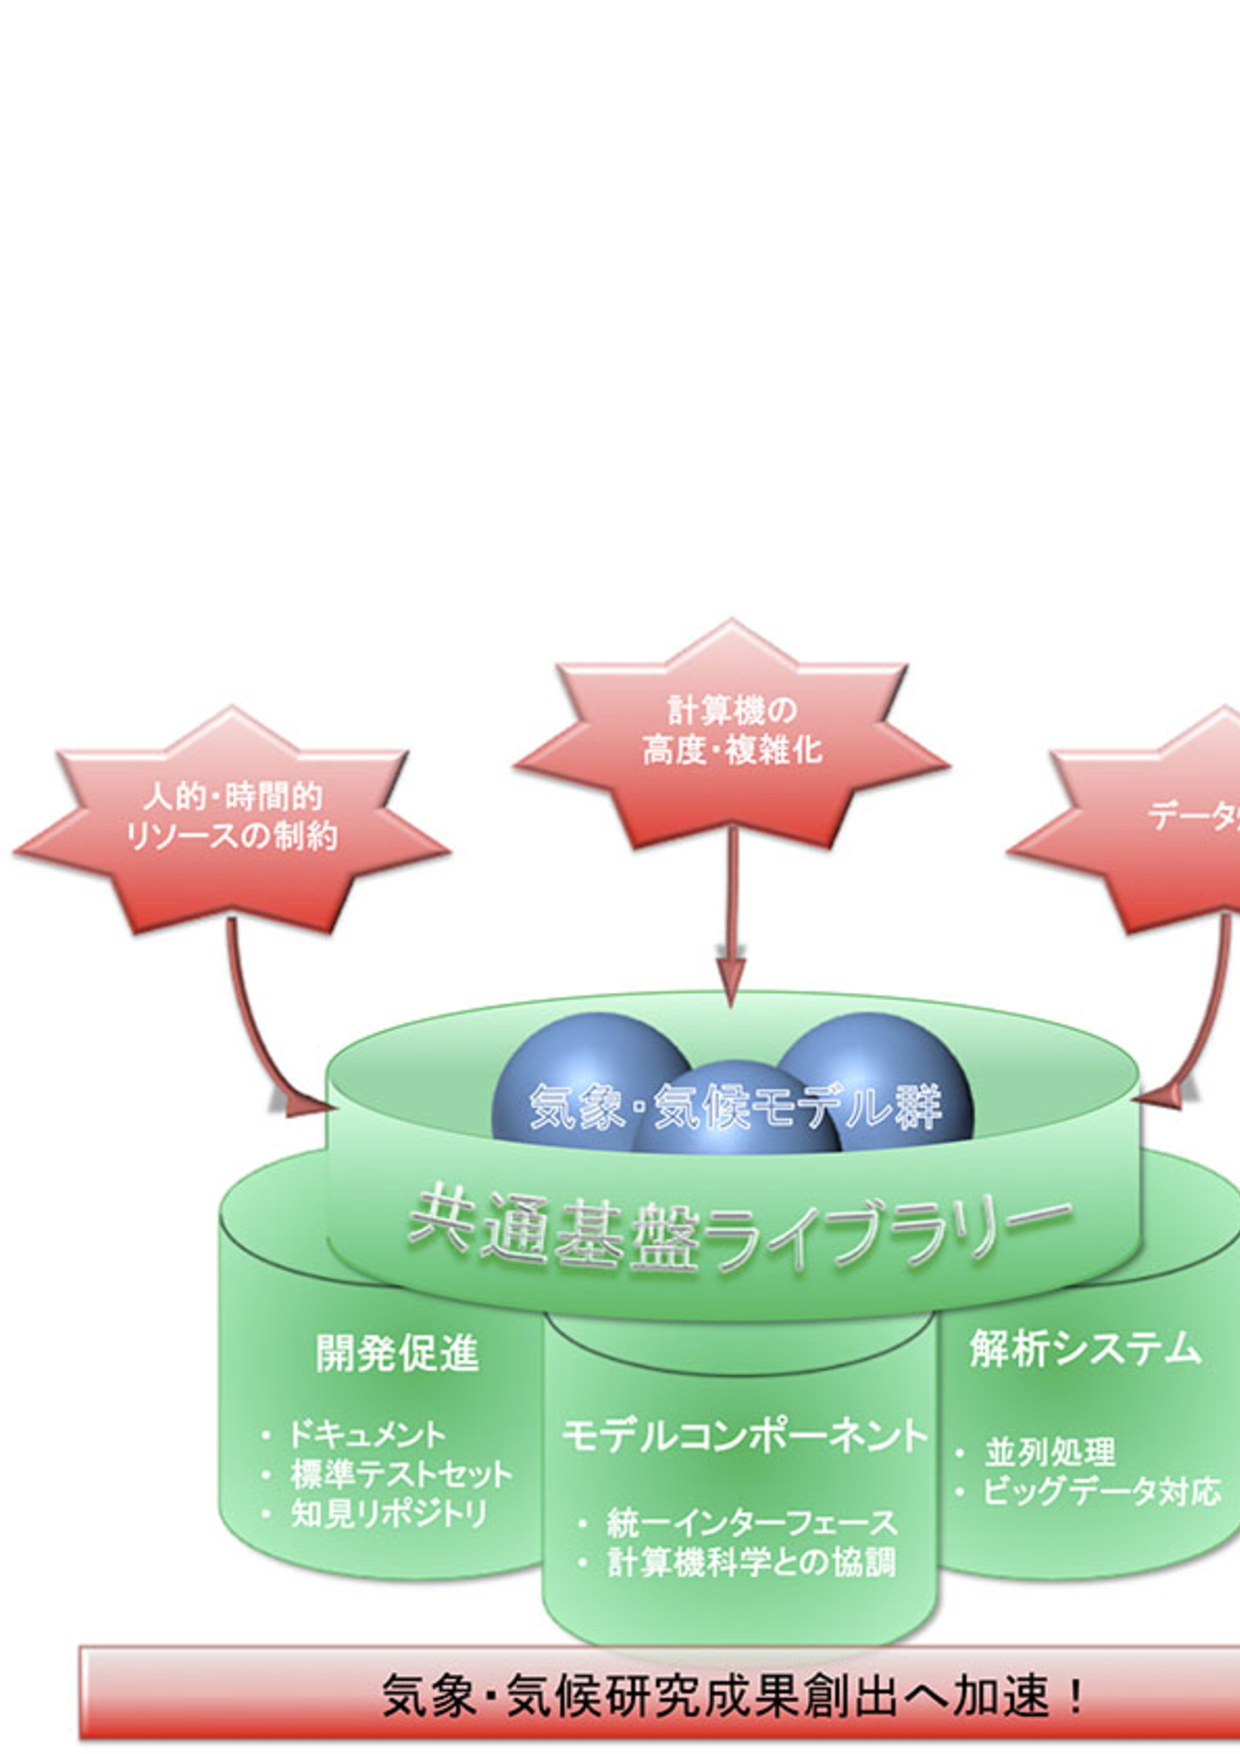
\includegraphics[width=0.9\hsize]{./../../figure/library.pdf}\\
  \caption{Aims of \scalelib}
  \label{fig:scale}
\end{center}
\end{figure}

\scalelib was developed in RIKEN with several outside contributors,
and its improvement and extension continue.
Figure \ref{fig:scale} shows the schematic concept of \scalelib.
As shown in this figure, SCALE aims to resolve various problems.
The development of \scalelib is considered in the context of its wide use
by devices ranging from small PC clusters to next-generation supercomputers.
For this purpose, scientists in meteorology/climate science
and computer science are cooperating.
%This has led to high computational performance of SCALE not only in supercomputers,
%such as the K Computer and the Fujitsu FX10,
%but also for general-purpose commercial computers,
%such as Intel processor-based machines.

\scalerm is a numerical model that fully uses \scalelib.
This model is contained in the \scalelib package,
as shown in Fig. \ref{fig:scale-rm}.
\scalelib manages the parallel processes,
file I/O, and inner-communication.
\scalelib also provides the solver for atmospheric flow ( dynamical core )
and physical processes such as micro-physics and radiation processes.
On the other hand,
\scalerm is constructed by combining functions provided by \scalelib.
\scalerm itself reads the input data of atmospheric status as prognostic variable,
and conducts time-integration.
Users can select a scheme in every component according to simulations they want.

\begin{figure}[hbt]
\begin{center}
  \includegraphics[width=0.9\hsize]{./../../figure/scale.pdf}\\
  \caption{Relationship between the library \scalelib and the model \scalerm}
  \label{fig:scale-rm}
\end{center}
\end{figure}


\section{Structure of \scalerm}  \label{subsec:sturcture_scale_rm}
%--------------------------------------------------------------%
All schemes in all components of \scalelib are available in \scalerm.
The components are categorized into three parts:
framework, dynamical core, and physical processes.
Components with various schemes already implemented
in the current version of \scalerm are listed below\footnote{Refer to \citet{scale_2015},\citet{satoy_2015b}, and \citet{nishizawa_2015} for the details of the model structure and the discretization method.}.

\subsubsection{Framework}
\begin{itemize}
 \item The three-dimensional (3D) Cartesian grid system based on actual distance
 \item 2D domain decomposition by Message Passing Interface (MPI) communication
 \item Several map projections commonly used
 \item Domain nesting system ( one-way, i.e., data transfer from parent domain to child domain. )
   \begin{itemize}
    \item  On-line nesting: concurrent execution of multiple domains).
    \item  Offline nesting: execution of computation in an inner domain after that in an outer domain.
   \end{itemize}
 \item Collective execution system of multiple cases, i.e., bulk job system
 \item \netcdf file I/O based on CF (Climate and Forecast) convention\footnote{\url{http://cfconventions.org/}}
   \begin{itemize}
   \item Selection of {\netcdf}3 and {\netcdf}4 formats
   \end{itemize}
 \item Generation of initial data for an ideal experiment
 \item Generation of topographical and land-use data, converted from external data
 \item Generation of initial and boundary data from external data
   \begin{itemize}
    \item 
      Supporting inputs from the WRF-ARW\footnote{\url{http://www.wrf-model.org/}} and
      \grads \footnote{\url{http://cola.gmu.edu/grads/}} formats.
   \end{itemize}
\end{itemize}

\subsubsection{Dynamical core}
\begin{itemize}
 \item Governing equations: 3D fully compressible non-hydrostatic equations
 \item Spatial discretization: finite volume method
    \begin{itemize}
      \item central advection schemes with 2nd-, 4th-, 6th-order, and 8th-order accuracy
      \item upwind advection schemes with 3rd- , 5th-order, and 7th-order accuracy
    \end{itemize}
 \item Time integration: selection from the ``fully explicit method'' (HEVE)
   or the ``horizontally explicit and vertically implicit methods'' (HEVI)
    \begin{itemize}
      \item \citet{Wicker_2002}'s 3 stage Runge--Kutta scheme with generally 2nd order accuracy
      \item Heun-type 3 stage Runge--Kutta scheme with 3rd order accuracy
      \item 4 stage Runge--Kutta scheme with 4th order accuracy
      \item 7 stage Runge--Kutta scheme with 6th order accuracy (supported only for HEVE)
      \item 11 stage Runge--Kutta scheme with 8th order accuracy (supported only for HEVE)
    \end{itemize}
 \item Guarantee of non-negative value:
    \begin{itemize}
      \item Flux corrected transport method \citep{zalesak_1979}
      \item \citet{Koren_1993}'s filter: available only with the use of the 3rd-order upwind advection scheme
    \end{itemize}
 \item Numerical filter: hyper-viscosity and diffusion with 2nd, 4th, 6th and 8th-order differential operators 
 \item Topography: expressed using terrain-following coordinates
\end{itemize}


\subsubsection{Physical processes}
\begin{itemize}
\item Turbulence process: selectable from among the following
  \begin{itemize}
  \item \citet{smagorinsky_1963} \& \citet{lilly_1962}-type sub-grid scale turbulent model
    with the corrections by \citet{Brown_etal_1994} and \citet{Scotti_1993}
  \item \citet{Deardorff_1980} sub-grid scale turbulent model
  \item MYNN level 2.5 boundary scheme ( \citet{my_1982,nakanishi_2004} )
  \end{itemize}
\item Cloud microphysics: selectable from among the following
  \begin{itemize}
  \item 3-class 1 moment bulk scheme \citep{kessler_1969}
  \item 6-class 1 moment bulk scheme \citep{tomita_2008}
  \item 6-class 2 moment bulk scheme \citep{sn_2014}
  \item spectral bin scheme \citep{suzuki_etal_2010}
  \end{itemize}
\item Radiation process: a k-distribution-based broadband radiation transfer model ( \citet{sekiguchi_2008} )
\item Surface models
  \begin{itemize}
  \item Land model: heat diffusion/bucket model
  \item Ocean model: selectable from among the following
    \begin{itemize}
    \item fixed to initial condition
    \item input from external data
    \item slab model
    \end{itemize}
  \item Urban model: a single-layer canopy model \citep{kusaka_2001}
  \item Heat transfer coefficient at land and in ocean: selectable from among the following
    \begin{itemize}
    \item The bulk method using the universal function \citep{beljaars_1991,wilson_2001}
    \item Louis-type bulk method \citep{uno_1995}
    \end{itemize}
  \end{itemize}
\end{itemize}

\section{Notations used in this document} \label{sec:notation}

This document assumes an execution in the shell ``bash'' on some Unix system.
If your environment is different, replace the commands
by the relevant commands suitable for your environment.
Unless there is a particular remark, this documentation obeys the following notation:

The command-line symbol for execution is expressed by \verb|$| or \verb|#|.
The difference between the two notations is 
in the permission levels of program execution, as shown below:
\begin{verbatim}
 #        <- command by root permission
 $        <- command by user permission
\end{verbatim}

A description enclosed in a rectangle expresses a message generated by the command line, as shown below.
\msgbox{
 -- -- -- -- command-line message\\
 -- -- -- -- -- -- -- -- command-line message\\
 -- -- -- -- -- -- -- -- -- -- -- -- command-line message\\
}

On the other hand, a description enclosed in a polygon with rounded corners means that the description is in an editable file.
\editbox{
 -- -- -- -- description in a file\\
 -- -- -- -- -- -- -- -- description in a file\\
 -- -- -- -- -- -- -- -- -- -- -- -- description in a file\\
}

In this documentation, the FORTRAN namelist and its items are denoted by
\namelist{\it namelist} and \nmitem{\it item_of_namelist}, respectively.



\chapter{Install} \label{chap:install}
ここでは,日本域を対象とした実事例実験のチュートリアルを通して,SCALE-LESモデルを実行する一連の作業を説明する.


\section{Installation of SCALE-LES}
%####################################################################################

ここでは,SCALE-LESモデルパッケージを含むSCALEライブラリの
インストール方法を説明する.
SCALEライブラリのインストールに必要となるライブラリ環境のインストール方法については,
必要に応じてAppendix \ref{sec:env_setting}を参照して事前にインストールすること.
以降のチュートリアルでは,Ruby DCL/GPhysに含まれるgpviewがインストールされていると想定して描画の説明を行う.
SCALEのインストールにはコマンドライン端末を使う.コマンドラインのシンボル(\verb|$|)があれば、コマンドの実行を示す.


\subsection{Required Environment}
%====================================================================================

\begin{itemize}
  \item {\bf 計算機環境} : Linux互換OS (Mac OS-Xを含む)が動作する環境.
        マルチコアCPU環境以上を推奨する.
        実験サイズによるが4GB以上のメモリがインストールされているマシン環境が好ましい.
  \item {\bf OS} : Linux OS(Fedora, CentOS, SUSE等),Max OS-X.ここではLinux (CentOS7)を使用して説明する.
  \item {\bf コンパイラ} : Fortran 2003をサポートするC,Fortranコンパイラを必要とする.
        GNU 4.6.x以上,Intel compiler 2012以上を推奨する.ここでは,gcc/gfortranを使用して説明する.
  \item {\bf MPIライブラリ} : MPICH2, OpenMPI, Intel MPI等をサポートする.ここではopenMPIを使用して説明する.
  \item {\bf netcdf3 もしくは HDF5/netcdf4} : gzip, szipをサポートするHDF5,
        およびそのHDF5をサポートするnetcdf4を必要とする.
        ただし,netcdf3の環境下ではscaleライブラリが提供する全ての機能をサポートできない可能性がある.
  \item {\bf 描画環境(非必須)} : Dennou Club提供のRuby DCL/GPhysに含まれるgpview,
        もしくはGrads等の描画環境があると計算結果を簡単にチェックできる.gpviewの使用を推奨する.
  \item SCALEは演算性能評価のためにPAPIライブラリを使用が可能です.
        PAPIライブラリがインストールされている環境下では,
        以下で説明するconfigureファイルの編集によってPAPIを適用することができます.
\end{itemize}



\subsection{Building the source code} \label{sec:source_code}
%====================================================================================

\subsubsection{ソースコードの入手}
%-----------------------------------------------------------------------------------

\url{http://scale.aics.riken.jp/download/scale.tar.gz} の安定版ソースコードのtarballをダウンロードすることができる.
ソースコードのtarballファイルを展開すると\verb|scale/|というディレクトリができる.
以降の説明で\verb|${TOPDIR}|は,scaleディレクトリが存在する絶対PATHを差す.

実事例のシミュレーションを行うには,ソースコードに加えて外部データが必要になる.
このチュートリアル用の気象場のデータ,日本領域の地形・土地利用のデータが収められた
\url{http://scale.aics.riken.jp/download/tutorial_data.tar.gz}も入手し,\verb|${TOPDIR}|の下,
つまりscaleディレクトリと同じ場所に展開しておくこと.\\
\begin{itemize}
 \item \verb|tutorial_data/input_atom| に気象場データ,\\
 \item \verb|tutorial_data/input_topo| に地形データ,\\
 \item \verb|tutorial_data/input_landuse| に土地利用データ\\
\end{itemize}
がそれぞれ格納されている.

\verb|tutorial_data|には,本チュートリアルに必要な最低限のデータのみが納めされているため,
その他の設定で実験を行う場合には別途,気象場,地形,および土地利用データが必要となる.


\subsubsection{configure ファイルと環境変数の設定}
%-----------------------------------------------------------------------------------

\verb|scale/sysdep|内にいくつかのコンフィグファイル(\verb|Makedef.***|)が準備されている.
これらの内から自分の環境にあったものを設定する.
ここでは,OSはLinux,gcc/gfortran コンパイラ,およびopenMPIを使用するため,
\verb|"Makedef.Linux-gnu-ompi"|が設定すべきコンフィグファイルである.
自分の環境に合うものがなければ既存ファイルをベースにして作成する必要がある.
\verb|Makedef.***|の\verb|"***"|の部分を下記のように環境変数として設定する.
\verb|.bashrc|などのファイルに記述しておくと便利である.

また、現実実験のための地形データ、
SCALEをコンパイルするのに必要な外部ライブラリについても下記のようにPATHを設定する.
ここでは,Appendix \ref{sec:env_setting}に従ったとして,
HDF5,netcdf4ともに\verb|/usr|の下にインストールされている場合の例を示す.

\begin{verbatim}
 $ export SCALE_SYS="Linux-gnu-ompi"
 $ export HDF5="/usr"
 $ export NETCDF4="/usr"
\end{verbatim}


\subsubsection{コンパイル}
%-----------------------------------------------------------------------------------

下記のディレクトリに移動して,makeコマンドによってコンパイルを行う.
\begin{verbatim}
 $ cd scale-les/test/tutorial/bin
 $ make -j 4
\end{verbatim}

\verb|make|のあとの \verb|"-j 4"| は,並列コンパイルを指示するオプションで,4並列コンパイルを行うことを指示する.
コンパイルを実行する環境によっては並列数を増やすこともできる.

このmakeによってSCALEライブラリ,およびSCALE-LESモデルのコンパイルが行われ,結果として
\verb|scale-les, scale-les_init, scale-les_pp|の3つの実行ファイルが生成されていればコンパイルは成功である.


{\bf 注意点}
\begin{itemize}
\item SCALEライブラリは,scaleのTOPディレクトリ直下の\verb|scale/scalelib/|というディレクトリ内でコンパイルと
アーカイブが行われ,\verb|"./lib"|という名前の隠しディレクトリとして\verb|bin/|ディレクトリ内へコピーされている.\\
\item Debugモードでコンパイルしたい場合や,コンパイルオプションを変更したい場合は,
      \verb|Makedef.***|のファイルを編集してください.
\item 開発版ソースコードをコンパイルしている場合,一部のコンパイラバージョンにおいて
      コンパイルが正常に終了しないケースがあります.そのような場合はぜひSCALE開発チームまでご報告ください.
\end{itemize}



%####################################################################################



\chapter{Operation check and basic usage} \label{chap:tutorial_ideal}
%%%%%%%%%%%%%%%%%%%%%%%%%%%%%%%%%%%%%%%%%%%%%%%%%%%%%%%%%%%%%%%%%%%%%
%  File 31_ideal_exp.tex
%%%%%%%%%%%%%%%%%%%%%%%%%%%%%%%%%%%%%%%%%%%%%%%%%%%%%%%%%%%%%%%%%%%%%
\section{概要} \label{sec:ideal_exp_intro}

本章では、まずSCALE-RMを使ってみるための基本的な操作について説明する。
第\ref{chap:install}章で実行したSCALEのコンパイルが正常に完了しているか
どうかのチェックも兼ねているのでぜひ実施してもらいたい。

%%  ====2章に書いてあるので削除した。
%% \subsubsection{本章を実行するための推奨環境}

%% 本章の説明は、下記の環境を前提として記述している。
%% コンパイラ、ライブラリについては、適宜、使用環境に合わせて読み替えること。

%% \begin{itemize}
%%  \item {\bf CPU} : 物理コアが2コア以上 %[Intel Core i5 2410M 2.3GHz 2コア/4スレッド] %、第\ref{chap:tutorial_real}章は4コアを搭載
%%  \item {\bf Memory} : 512MB以上 %[DDR3-1333 4GB]     %、第\ref{chap:tutorial_real}章は2GB
%%  \item {\bf OS} : Linux OS x86-64  %[CentOS 6.6、CentOS 7.1、openSUSE 13.2のいずれか]
%%  \item {\bf コンパイラ} : GNU コンパイラ(gcc/gfortran)
%%  \item {\bf MPIライブラリ} : openMPI(リポジトリ経由でのインストール)
%% \end{itemize}

本章では、SCALEのコンパイルが正常に終了し、
すでに下記のファイルが生成されているものとして説明を行う。
\begin{alltt} 
  scale-{\version}/scale-rm/test/tutorial/bin/scale-rm
  scale-{\version}/scale-rm/test/tutorial/bin/scale-rm_init
  scale-{\version}/scale-rm/util/netcdf2grads_h/net2g
\end{alltt}
これらに加えて、描画ツールとして\grads を使用する。
gpviewは、結果の確認用に利用することができる。
\grads およびgpview(GPhys)との詳細やインストール方法については、
付録 \ref{sec:env_vis_tools}節を参照のこと。





\section{実行方法} \label{sec:ideal_exp_run}
%====================================================================================

実行の流れとしては、前準備、初期値の作成、モデル本体の実行、
後処理、そして描画といった順番で作業を進める。

\subsection{前準備} \label{subsec:ideal_exp_prepare}
%------------------------------------------------------
チュートリアル理想実験は、\verb|scale-rm/test/tutorial/ideal|の
ディレクトリにて実行する。
\begin{alltt}
  $ cd scale-rm/test/tutorial/ideal
\end{alltt}
次に、このディレクトリに、
SCALEの実行バイナリの静的リンクを張る。
\begin{alltt}
  $ ln -s ../bin/scale-rm       ./
  $ ln -s ../bin/scale-rm_init  ./
\end{alltt}
``\verb|scale-rm|''はモデル本体、
``\verb|scale-rm_init|''は初期値・境界値作成ツールである。
%もし、ここで説明するディレクトリとは異なる場所で実行している場合は、
%リンクを張る時のディレクトリ指定に注意すること。


\subsection{初期値作成} \label{subsec:ideal_exp_init}
%------------------------------------------------------
初期値の作成は、``\verb|scale-rm_init|''に
設定ファイルを与えて実行する。
``\verb|init_R20kmDX500m.conf|''には、
表\ref{tab:setting_ideal}に対応した実験設定が書き込まれている。
この設定ファイルを\verb|scale-rm_init|に与えることで、
設定ファイルの指示に従って大気の成層構造を計算し、
初期擾乱が設定される。


SCALEの基本的な実行コマンドは下記のとおりである。
\begin{alltt}
  $ mpirun  -n  [プロセス数]  [実行バイナリ名]  [設定ファイル]
\end{alltt}
[プロセス数]の部分にはMPI並列で使用したいプロセス数を記述する。
[実行バイナリ]には、\verb|scale-rm|や\verb|scale-rm_init|が入る。
そして、実験設定を記述した設定ファイルを
[設定ファイル]の部分に指定する。
%
例えば、
設定ファイルに\verb|init_R20kmDX500m.conf|を用いて、
2-MPI並列(2つのMPIプロセス)
で\verb|scale-rm_init|を実行する場合、
コマンドは次のようになる。
\begin{alltt}
  $ mpirun  -n  2  ./scale-rm_init  init_R20kmDX500m.conf
\end{alltt}
%
\noindent 実行が成功した場合には、コマンドラインのメッセージは
下記のように表示される。\\

\noindent {\small {\gt
\fbox{
\begin{tabularx}{140mm}{l}
 *** Start Launch System for SCALE-RM\\
 *** Execute preprocess? :  T\\
 *** Execute model?      :  F\\
 *** a single comunicator\\
 *** a single comunicator\\
\end{tabularx}
}}}\\


\noindent この実行によって、
\begin{alltt}
  init_LOG.pe000000
  init_00000101-000000.000.pe000000.nc
  init_00000101-000000.000.pe000001.nc
\end{alltt}
の3つのファイルが、現在のディレクトリ下に作成される。
``init\_LOG.pe000000''には、
コマンドラインには表示されない詳しい実行ログが記録されている。
実行が正常に終了している場合、このLOGファイルの最後に\\

\noindent {\small {\gt
\fbox{
\begin{tabularx}{140mm}{l}
 ++++++ Stop MPI\\
 \\
 *** MPI is peacefully finalized\\
\end{tabularx}
}}}\\

\noindent と記述される。

\verb|init_00000101-000000.000.pe000000.nc|と\verb|init_00000101-000000.000.pe000001.nc|の
2つのファイルは初期値ファイルである。
計算領域全体を2つのMPIプロセスで分割し担当するため、
2つのファイルが生成される。
もし、4-MPI並列で実行すれば、4つの初期値ファイルが生成される。
これらのファイル名の末尾が``.nc''で終わるファイルは
NetCDF形式のファイルであり、
GPhys/Ruby-DCLやncviewといったツールで直接読むことができる。


\subsection{モデル本体の実行} \label{subsec:ideal_exp_run}
%------------------------------------------------------
並列数は、初期値作成のときと同じ数を指定する。
設定ファイルには``\verb|run_R20kmDX500m.conf|''を指定する。
\begin{alltt}
  $ mpirun  -n  2  ./scale-rm  run_R20kmDX500m.conf
\end{alltt}

本書の必要要件にあった計算機であれば、2分程度で計算が終わる。
\noindent この実行によって、\\
\begin{alltt}
  LOG.pe000000
  history.pe000000.nc
  history.pe000001.nc
\end{alltt}
の3つのファイルが、現在のディレクトリ下に作成されているはずである。
``LOG.pe000000''には、
コマンドラインには表示されない詳しい実行ログが記録されている。
実行が正常に終了している場合、このLOGファイルの最後に\\

\noindent {\small {\gt
\fbox{
\begin{tabularx}{140mm}{l}
 ++++++ Stop MPI\\
 \\
 *** MPI is peacefully finalized\\
\end{tabularx}
}}}\\

\noindent と記述される。
``history.pe000000.nc''と``history.pe000001.nc''
の2つのファイルが計算結果が記録されたhistoryファイルである。
2-MPI並列で実行したため、2つのファイルが生成されており、
ファイル形式はNetCDFである。
%``monitor.pe000000''は、計算中にモニタリングしている
%物理変数の時間変化を記録したテキストファイルである。


\section{後処理と描画} \label{sec:ideal_exp_net2g}
%------------------------------------------------------
ここでは、後処理と計算結果の描画方法について説明する。本書のチュートリアルでは、
NetCDF形式の分散ファイルを1つのファイルにまとめ、ダイレクトアクセスが可能な
単純バイナリ形式(\grads 形式)に変換する方法を説明する。
このバイナリ形式は、ユーザーによる結果の解析を容易にする。
%GPhys/Ruby-DCLを使うと
%分割ファイルのまま直接描画することができるが、この方法については\ref{sec:quicklook}節を
%参照してもらいたい。

まず、\ref{sec:source_net2g}節でコンパイルした後処理ツール\verb|net2g|へリンクを張る。
\begin{verbatim}
  $ ln -s ../../../util/netcdf2grads_h/net2g  ./
\end{verbatim}
%もし、ここで説明するディレクトリとは異なる場所で実行している場合は、
%リンクを張る時のディレクトリ指定に注意すること。

\verb|net2g| の実行方法は、基本的に{\scalerm}と同じであり、
\begin{verbatim}
  $ mpirun  -n  [プロセス数]  ./net2g  [設定ファイル]
\end{verbatim}
の形式で実行する。
net2g専用の \verb|net2g_R20kmDX500m.conf|を設定ファイルとして与えて、
次のように実行する。
\begin{verbatim}
  $ mpirun  -n  2  ./net2g  net2g_R20kmDX500m.conf
\end{verbatim}
エラーメッセージがなく、下記のメッセージだけが標準出力へ表示されていれば、正常に変換は完了している。\\

\noindent {\gt
\fbox{
\begin{tabularx}{150mm}{l}
\verb|+++ MPI COMM: Corrective Finalize| \\
\end{tabularx}
}}\\

\noindent net2gの実行には、{\scalerm}の実行時に使用したMPIプロセス数と同じか、
その約数のプロセス数を使用しなければならない。
%HDDの読み書き速度に依存するが、本書の必要要件にあった計算機であれば2分程度で計算が終わる。
この実行によって、実行ディレクトリ下に下記6つのファイルが作成される。
\begin{alltt}
  QHYD_d01z-3d.ctl
  QHYD_d01z-3d.grd
  U_d01z-3d.ctl
  U_d01z-3d.grd
  W_d01z-3d.ctl
  W_d01z-3d.grd
\end{alltt}
「grd」ファイルは、分割ファイルを結合することによって得られる、
ダイレクトアクセス可能の単純バイナリ形式(\grads 形式)である。
一方、「ctl」ファイルは、\grads によって「grd」ファイルを読む込むときに必要な情報を含む。

計算が問題なく完了しているかを確認するため、\grads スクリプト \verb|checkfig_ideal.gs|
を使って作図する。なお、\grads のバージョンによって文法が異なるため、
警告が出る場合には\grads スクリプトを適宜変更されたい。
\begin{verbatim}
  $ grads -blc checkfig_ideal.gs
\end{verbatim}
作図が成功すると、下記の図が生成される。
\begin{verbatim}
   ideal_QHYD.png
   ideal_W.png
\end{verbatim}
シミュレーションと後処理が成功していれば、図\ref{fig_ideal}と同じ図が得られる。

\begin{figure}[t]
\begin{center}
  \includegraphics[width=0.7\hsize]{./figure/ideal_qhyd.eps}\\
  \includegraphics[width=0.7\hsize]{./figure/ideal_W.eps}\\
  \caption{積分開始から 1200 秒(20 分)後の Y=750 mにおける東西-鉛直断面図;
           カラーシェードは、(a)において全質量に対する凝結物の質量比、
           (b)において鉛直速度を表す。ベクトルは東西-鉛直断面内の風の流れを表す。}
  \label{fig_ideal}
\end{center}
\end{figure}


他の変数についてもバイナリデータに変換したい場合には、
\verb|net2g_R20kmDX500m.conf|の\namelist{VARI}の\nmitem{VNAME} に必要な変数を追加すればよい。\\

\noindent {\small {\gt
\ovalbox{
\begin{tabularx}{150mm}{l}
\verb|&VARI|\\
\verb| VNAME       = "U","W","QHYD"|\\
\verb|/|\\
\end{tabularx}
}}}\\

\noindent
historyファイルに出力されている変数は、{\netcdf} の\verb|ncdump| などを
使えば簡単に確認できる。net2gの詳しい使用方法は、第\ref{sec:net2g}節を参照されたい。





\section{Guideline for further study} \label{sec:ideal_exp_last}

In this chapter,
the method for the execution of \scalerm was explained by using a simple ideal experiment. We recommend studying methods of changing the model resolution, the calculation domain, and the number of MPI processes for further study.  With regard to the ideal experiment, several files of other configurations,  e.g., to increase resolution, the number of domains, and the physical scheme, are prepared in the directory ``sample'' under the same directory as was used in this experiment.  These configuration files are useful to change such configurations.  Moreover, various ideal experimental settings  have been prepared in the directory ``\verb|scale-rm/test/case|.'' For some ideal experiments,  it may be necessary to carry out the ``make'' command again in the same directory as in the configuration file  because some test cases need special source codes according to their experimental settings. The procedures for the generation of the initial conditions and those for simulation execution are the same as in the tutorial in this chapter.

It is important to study the method for the configuration of physical processes, such as cloud microphysics, radiation, and turbulence schemes. Methods to alter them in detail are described in Chapter \ref{chap:basic_usel}.



\chapter{Conduction of real atomsphere experiment} \label{chap:tutorial_real}
%-------------------------------------------------------%
\section{Overview} \label{sec:tutrial_real_intro}
%-------------------------------------------------------%
In this chapter, the basic execution procedure of the real atmospheric experiment is described using a simple case according to the workflow in Fig. \ref{fig:howto}.
\begin{enumerate}
\item Preparations for input data. The input data must be prepared by users themselves.
\item \texttt{pp}:   Making topographical data
\item \texttt{init}: Making initial and boundary data
\item \texttt{run}:  Executing the simulation
\item \texttt{net2g}: Converting {\netcdf} output data to {\grads} format ( optional )
\end{enumerate}
Hereinafter, the absolute path \texttt{scale-{\version}/scale-rm/test/tutorial/} is denoted by\\
\verb|${Tutorial_DIR}|.

\begin{figure}[tb]
\begin{center}
  \includegraphics[width=0.9\hsize]{./figure/real_procedure.eps}\\
  \caption{\scalerm procedure of model execution}
  \label{fig:howto}
\end{center}
\end{figure}

The settings for the calculation domain used in this tutorial are given in Table \ref{tab:grids}.
Figure \ref{fig:tutrial_real_domain} shows the target domain.
Since this tutorial focuses on learning how to conduct 
real atmospheric experiments using \scalerm quickly,
the experiment is designed to be completed in a short time.
Note that this setting may not be appropriate as a physically valid experiment;
e.g., there is no cumulus parameterization in this simulation, even though the horizontal resolution is 20 km.

\begin{table}[tb]
\begin{center}
  \caption{Overview of experimental settings}
  \label{tab:grids}
  \begin{tabularx}{150mm}{|l|X|} \hline
    \rowcolor[gray]{0.9} Item & Configuration \\ \hline
    MPI process decomposition (east-west $\times$ north-south) & 2 $\times$ 2 (total: 4 processes) \\ \hline
    Number of horizontal grids (east-west $\times$ north-south) & 90 $\times$ 90  \\ \hline
    Number of vertical layers   & 36                   \\ \hline
    Horizontal grid intervals   & $\Delta x  = \Delta y = $ 20km       \\ \hline
    Integration period & July 14, 2007, 18UTC - July 15 00UTC (6 hour integration) \\ \hline
    Time step & 90 s/step (total:240 steps) \\ \hline
  \end{tabularx}
\end{center}
\end{table}

\begin{figure}[tb]
\begin{center}
  \includegraphics[width=1.0\hsize]{./figure/real_domain.eps}\\
  \caption{Topographical and land-ocean distribution in the domain}
  \label{fig:tutrial_real_domain}
\end{center}
\end{figure}



%-------------------------------------------------------%
\section{入力データ(境界データ)の準備} \label{sec:tutrial_real_data}
%-------------------------------------------------------%

現実大気実験のシミュレーションを行う場合、\scalerm 本体に与える
境界値データが必要になる。境界値データとしては表\ref{tab:real_bnd}
が必要である。{\color{blue}青字}は必須の変数、その他は任意である。

\begin{table}[h]
\begin{center}
  \caption{現実大気実験に必要な初期値境界値データ}
  \label{tab:real_bnd}
  \begin{tabularx}{150mm}{llX} \hline
    \multicolumn{3}{l}{地形データ(\scalerm の地形を用意する)}\\ \hline
    & \multicolumn{2}{l}{\color{blue}{標高データ}}\\
    & \multicolumn{2}{l}{\color{blue}{土地利用区分データ}}\\ \hline
    \multicolumn{3}{l}{初期値境界値データ}\\ \hline
    &  \multicolumn{2}{l}{\color{blue}{親モデルの緯度・経度}}\\
    &  \multicolumn{2}{l}{(3次元大気データ)}\\
    & &  \multicolumn{1}{l}{\color{blue}{東西風速, 南北風速, 気温, 比湿(相対湿度), 気圧, ジオポテンシャル高度}} \\
    &  \multicolumn{2}{l}{(2次元大気データ)}\\
    & & 海面更正気圧, 地上気圧, 10m東西風速, 10m南北風速, 2m気温, 2m比湿(相対湿度) \\
    &  \multicolumn{2}{l}{(2次元陸面データ)}\\
    & &  \multicolumn{1}{l}{親モデルの海陸マップ}\\
    & &  \multicolumn{1}{l}{\color{blue}{地表面温度(Skin temp)}}\\
    & &  \multicolumn{1}{l}{{\color{blue}{親モデル土壌データの深さ情報, 土壌温度}}, 土壌水分(体積含水率 or 飽和度)}\\
    &  \multicolumn{2}{l}{(2次元海面データ)}\\
  & &  \multicolumn{1}{l}{\color{blue}{海面水温(Skin tempがある場合は省略可)}}\\ \hline
  \end{tabularx}
\end{center}
\end{table}

\proofcomment{(八代)表4.2は変換に必要な外部データのリストですか?それとも変換後の入力データのリストですか?} \\
\proofcomment{(八代)\scalerm の地形という言葉が曖昧です。}


\subsubsection{標高データと土地利用区分データ}
標高データと土地利用区分データは実験設定に従って、
\scalerm のそれぞれの格子点における標高、海陸比率、湖比率、都市被覆率、植生比率、土地(植生)利用区分を
作成するために使用する。
ユーザーが全球の任意の地域を対象とした計算ができるよう、
フォーマット変換済みの
標高データ USGS(U.S. Geological Survey) のGTOPO30 と、
土地利用区分データ GLCCv2 を提供している。
%これらのデータベースを作成にするにあたり、施された前処理手順の詳細については、〇〇を参照すること(Todo)。

\begin{enumerate}
\item データのダウンロード\\
\scalerm 用の標高・土地利用区分のデータを\\
 \url{http://scale.aics.riken.jp/download/scale_database.tar.gz}\\
より入手し、任意のディレクトリに展開しておく。
\begin{alltt}
  $ tar -zxvf scale_database.tar.gz
\end{alltt}
展開したディレクトリには、標高データと土地利用区分データが格納されている。
\begin{alltt}
  scale_database/topo/    <- 標高データ
  scale_database/landuse/ <- 土地利用区分データ
\end{alltt}

\item パスの設定\\
makeを用いたジョブスクリプト生成を利用するためには、
展開先のディレクトリを \verb|SCALE_DB| という環境変数に設定しておくことが必須である
(以後、\verb|${SCALE_DB}|と表記)。
データベースがあるディレクトリを
\begin{alltt}
  $ export SCALE_DB="${path_to_directory_of_scale_database}/scale_database"
\end{alltt}
\end{enumerate}
ここで、\verb|${path_to_directory_of_scale_database}|は、
データベースがあるディレクトリである。

\subsubsection{大気・陸面・海面水温データ}
初期値境界値データは4byteバイナリー(\grads 形式、以降''binary形式''と表記する)に変換すれば、
任意のデータを読み込むことが可能である。
基本的に、バイナリーデータはユーザー自身が用意する。
チュートリアルではNCEP FNL(Final) Operational Global Analysis data を使用する方法を示す。
あらかじめ\verb|wgrib|をインストールしておく\footnote{\url{http://www.cpc.ncep.noaa.gov/products/wesley/wgrib.html}}。

\begin{enumerate}
\item データのダウンロード\\
NCARのサイト
\url{http://rda.ucar.edu/datasets/ds083.2/}\\
から、2007年7月14日18時から一日分のgrib1フォーマットのデータ
\begin{alltt}
 fnl_20070714_18_00.grib1
 fnl_20070715_00_00.grib1
 fnl_20070815_06_00.grib1
 fnl_20070815_12_00.grib1
\end{alltt}
を\verb|scale-|{\version}\verb|/scale-rm/test/tutorial/real/tools/|の下にダウンロードする。

\item データフォーマットをgrib形式からbinary形式に変換\\
 \verb|scale-|{\version}\verb|/scale-rm/test/tutorial/real/tools/| の中にある \verb|convert_grib2grads_FNLgrib1.sh|を実行。

\begin{alltt}
 $ cd ${Tutorial_DIR}/real/tools/
 $ sh convert_grib2grads_FNLgrib1.sh
\end{alltt}
成功すれば、下記のファイルが作成される。
\begin{alltt}
 $ ls FNL_output/*/*
    FNL_output/200707/FNLatm_2007071418.grd
    FNL_output/200707/FNLatm_2007071500.grd
    FNL_output/200707/FNLatm_2007071506.grd
    FNL_output/200707/FNLatm_2007071512.grd
    FNL_output/200707/FNLland_2007071418.grd
    FNL_output/200707/FNLland_2007071500.grd
    FNL_output/200707/FNLland_2007071506.grd
    FNL_output/200707/FNLland_2007071512.grd
    FNL_output/200707/FNLsfc_2007071418.grd
    FNL_output/200707/FNLsfc_2007071500.grd
    FNL_output/200707/FNLsfc_2007071506.grd
    FNL_output/200707/FNLsfc_2007071512.grd
\end{alltt}
\end{enumerate}


%-------------------------------------------------------%
\section{実験セットの準備} \label{sec:tutrial_real_prep}
%-------------------------------------------------------%

現実大気実験では、理想実験と比べて多くの実行手続きやファイルが必要である。
加えて、前処理\verb|pp|、初期値作成\verb|init|、シミュレーション実行\verb|run|
で使用する設定ファイル(\verb|***.conf|)内の実験設定を統一する必要がある。
準備段階におけるファイルの不足や設定の不一致は、モデルが正常に動かない原因となる。
このような状況を回避するために、必要なファイル一式を生成するためのツール
「実験セット一式作成ツール」が用意されている。
まずはじめに、
以下のディレクトリに移動し、
次の手続きにより現実大気実験チュートリアルのためのファイル一式を用意する。
\begin{alltt}
 $ cd ${Tutorial_DIR}/real/
 $ ls
    Makefile : 実験セット一式作成のためのMakefile
    README   : スクリプトの使用に関する README
    USER.sh  : 実験設定の記述
    config/  : 一連のファイルの作成に対する各々の設定
              (基本的に、ユーザは書き換える必要はない)
    sample/  : USER.sh のサンプルスクリプト
    data/    : チュートリアルのためのツール類
    tools/   : チュートリアル用の初期条件のためのツール
              (チュートリアルの場合を除いて、基本的に各自で準備する)
 $ make
 $ ls experiment/    : このディレクトリは make により追加される
    init/
    net2g/
    pp/
    run/
\end{alltt}
\verb|make|を実行すると、\verb|USER.sh|に記述された設定に従って
\verb|experiment|ディレクトリの下に実験セットが作成される。
実験セット一式準備ツールに関する詳しい説明については、
第\ref{sec:basic_makeconf}節を参照いただきたい。
%なお、\verb|sample|ディレクトリにはネスティングの際に利用できるファイルが用意されており、
%必要に応じて参考にされたい。


%-------------------------------------------------------%
\section{地形・土地利用データの作成:pp} \label{sec:tutrial_real_pp}
%-------------------------------------------------------%

ppディレクトリへ移動し、現実実験のための地形データ、土地利用データを作成する。
\begin{verbatim}
 $ cd ${Tutorial_DIR}/real/experiment/pp/
 $ ls 
  pp.d01.conf scale-rm_pp
\end{verbatim}
ppディレクトリの中には、\verb|pp.d01.conf|という名前の
設定ファイルが準備されている。
ドメインの位置や格子点数など、実験設定に合わせて、
適宜\verb|pp.conf|を編集する必要があるが、
チュートリアルではすでに表\ref{tab:grids}の設定に
従って編集済みの\verb|pp.d01.conf|が用意されているため、
そのまま利用する。
\verb|pp.d01.conf|の設定の中で、
\namelist{PARAM_CONVERT}の中の以下の項目を確認してほしい。\\

\noindent {\gt
\ovalbox{
\begin{tabularx}{140mm}{l}
\verb|&PARAM_CONVERT| \\
\verb|  CONVERT_TOPO = .true.,| \\
\verb|  CONVERT_LANDUSE = .true.,| \\
\verb|/| \\
\end{tabularx}
}}\\

\noindent 上記のように\nmitem{CONVERT_TOPO}と\nmitem{CONVERT_LANDUSE}が
\verb|.true.|となっていることが、
それぞれ地形と土地利用の処理を行うことを意味している。
詳細な設定ファイルの内容については、付録\ref{achap:namelist}を参照されたい。

また、環境変数\verb|${SCALE_DB}|が適切に設定されている場合、
\namelist{PARAM_CNVTOPO_GTOPO30}の中の\nmitem{GTOPO30_IN_DIR}と
\namelist{PARAM_CNVLANDUSE_GLCCv2}の中の\nmitem{GLCCv2_IN_DIR}で設定されている
ディレクトリーに地形データと土地利用データの場所が適切に設定されているかどうかを
確認しておくこと。\\

\proofcomment{上記意味不明。環境変数で競ってしているのに、
なぜ、設定ファイルで設定しなおさねばならないのか???}


\noindent {\gt
\ovalbox{
\begin{tabularx}{140mm}{l}
\verb|&PARAM_CNVTOPO_GTOPO30| \\
\verb| GTOPO30_IN_CATALOGUE = "GTOPO30_catalogue.txt",|\\
\verb| GTOPO30_IN_DIR       = "./topo/GTOPO30/Products",|\\
\verb|/|\\
\\
\verb|&PARAM_CNVLANDUSE_GLCCv2|\\
\verb| GLCCv2_IN_CATALOGUE = "GLCCv2_catalogue.txt",|\\
\verb| GLCCv2_IN_DIR       = "./landuse/GLCCv2/Products",|\\
\verb| limit_urban_fraction = 0.3D0,|\\
\verb|/|\\
\end{tabularx}
}}\\


今回は、表\ref{tab:grids}に示されているように。
4つのMPIプロセスを使用する設定なので次のように実行する。
\begin{verbatim}
 $ mpirun -n 4 ./scale-rm_pp pp.conf
\end{verbatim}
%本節使用した環境において、実行にはおおよそ15秒を要する。
ジョブが正常に終了すれば、\verb|topo_d01.pe######.nc|と\\
\verb|landuse_d01.pe######.nc|と
いうファイルがMPIプロセス数だけ、つまり4つずつ生成される(
\verb|######|にはMPIプロセスの番号が入る)。
それぞれ、各格子点における地形と土地利用の情報が入っている。
実行時のログは、\verb|pp_LOG_d01.pe000000|に出力されるので内容を確かめておくこと。


%% サポート外
%% \vspace{1cm}
%% \noindent {\Large\em OPTION} \hrulefill \\
%% gpviewがインストールされている場合、次のコマンドによって、
%% 作成された地形と土地利用データが正しく作成されているかどうか
%% 確認することが出来る.正しく作成されていれば,図 \ref{fig:tutrial_real_domain}と同様の図ができる.
%% \begin{verbatim}
%%   $ gpview topo_d01.pe00000*@TOPO --aspect=1 --nocont
%%   $ gpview landuse_d01.pe00000*@FRAC_LAND --aspect=1 --nocont
%% \end{verbatim}


%-------------------------------------------------------%
\section{Creating the initial and boundary data: init} \label{sec:tutrial_real_init}
%-------------------------------------------------------%

Move to the directory \verb|init| and create the initial and boundary data for the \scalerm simulation as follows:
\begin{verbatim}
 $ cd ${Tutorial_DIR}/real/experiment/init
 $ ls
    init.d01.conf
    init.launch.conf
    param.bucket.conf
    scale-rm_init
\end{verbatim}

In the directory \verb|init|, there exists the configuration file \verb|init.d01.conf|.
The file \verb|init.launch.conf| also exists but is not used here.
It is necessary to edit the file \verb|init.d01.conf| according to such experimental settings as \verb|pp.d01.conf|. \verb|init.d01.conf| has been already edited for this tutorial experiment as shown in Table \ref{tab:grids}.  To create the initial and boundary data,  the topographical data generated in the previous section is used. This is set in \verb|init.d01.conf| to refer the relative path as follows:

\editbox{
\verb|&PARAM_TOPO| \\
\verb|   TOPO_IN_BASENAME = "../pp/topo_d01",| \\
\verb|/| \\
 \\
\verb|&PARAM_LANDUSE| \\
\verb|   LANDUSE_IN_BASENAME = "../pp/landuse_d01",| \\
\verb|/| \\
}
In particular,  the contents of \namelist{PARAM_MKINIT_REAL_ATMOS}, \namelist{PARAM_MKINIT_REAL_OCEAN} and \namelist{PARAM_MKINIT_REAL_LAND} are handled. It should be confirmed that the settings in \verb|init.d01.conf| are correct.
\editboxtwo{
\verb|&PARAM_MKINIT_REAL_ATMOS| & \\
\verb| NUMBER_OF_FILES      = 2,|                                   & {\small : number of files read } \\
\verb| FILETYPE_ORG         = "GrADS",|                             & {\small : choose from Table \ref{tab:inputdata_format}} \\
\verb| BASENAME_ORG         = "namelist.grads_boundary.FNL.grib1",| & \\
\verb| BASENAME_BOUNDARY    = "boundary_d01",|                      & {\small : output name of boundary data} \\
\verb| BOUNDARY_UPDATE_DT   = 21600.0,|                             & {\small : time interval of input data} \\
\verb| PARENT_MP_TYPE       = 3,|                                   & \\
\verb| USE_FILE_DENSITY     = .false.,|                             & {\small : use the atmospheric density in the parent model or not?} \\
\verb|/| \\
\\
\verb|&PARAM_MKINIT_REAL_OCEAN| & \\
\verb|   .........              |  & \\
\verb| INTRP_OCEAN_SFC_TEMP = "mask",|                              & {\small : how to treat the missing value of SST} \\
\verb| INTRP_OCEAN_TEMP     = "mask",|                              & {\small : how to treat the missing value of SST} \\
\verb|/| \\
\\
\verb|&PARAM_MKINIT_REAL_LAND| & \\
\verb|   ..........              | & \\
\verb| USE_FILE_LANDWATER   = .true.,|                              & {\small : use soil moisture data in the parent model or not?} \\
\verb| INTRP_LAND_TEMP      = "mask",|                              & {\small : how to treat the missing value of soil temperature} \\
\verb| INTRP_LAND_WATER     = "fill",|                              & {\small : how to treat the missing value of soil moisture} \\
\verb| INTRP_LAND_SFC_TEMP  = "fill",|                              & {\small : how to treat the missing value of surface temperate} \\
\verb|/| \\
}

The file format of the meteorological field data is specified in \nmitem{FILETYPE_ORG}. In this case, it is given as ``\grads'' to read data in \grads format. Refer to Section \ref{sec:adv_datainput} for the details of the input file.


Link the input data (FNL) that are converted into binary form in Section \ref{sec:tutrial_real_data} to the current working directory. A shell script for this appropriate linkage is prepared as \verb|"gradsinput-link_FNL.sh"| in the directory \verb|${Tutorial_DIR}/real/data|:
\begin{verbatim}
  $ cp ../../data/gradsinput-link_FNL.sh ./
  $ sh gradsinput-link_FNL.sh
\end{verbatim}
If the following linkages are found, it is successfully concluded.
\msgbox{
\verb|FNLatm_00000.grd -> ../tools/FNL_output/200707/FNLatm_2007071418.grd| \\
\verb|FNLatm_00001.grd -> ../tools/FNL_output/200707/FNLatm_2007071500.grd| \\
\verb|FNLatm_00002.grd -> ../tools/FNL_output/200707/FNLatm_2007071506.grd| \\
\verb|FNLatm_00003.grd -> ../tools/FNL_output/200707/FNLatm_2007071512.grd| \\
\verb|FNLland_00000.grd -> ../tools/FNL_output/200707/FNLland_2007071418.grd| \\
\verb|FNLland_00001.grd -> ../tools/FNL_output/200707/FNLland_2007071500.grd| \\
\verb|FNLland_00002.grd -> ../tools/FNL_output/200707/FNLland_2007071506.grd| \\
\verb|FNLland_00003.grd -> ../tools/FNL_output/200707/FNLland_2007071512.grd| \\
\verb|FNLsfc_00000.grd -> ../tools/FNL_output/200707/FNLsfc_2007071418.grd| \\
\verb|FNLsfc_00001.grd -> ../tools/FNL_output/200707/FNLsfc_2007071500.grd| \\
\verb|FNLsfc_00002.grd -> ../tools/FNL_output/200707/FNLsfc_2007071506.grd| \\
\verb|FNLsfc_00003.grd -> ../tools/FNL_output/200707/FNLsfc_2007071512.grd| \\
}

Then, link a namelist file to the directory \verb|init| to read the binary (\grads) data format in SCALE.
\begin{verbatim}
  $ ln -s ../../data/namelist.grads_boundary.FNL.grib1 ./
\end{verbatim}
After the above preparations, execute the \verb|scale-rm_init| using four MPI processes.
\begin{verbatim}
 $ mpirun -n 4 ./scale-rm_init init.d01.conf
\end{verbatim}

If the job finishes normally, the following files are generated:
\begin{verbatim}
 $ ls
    boundary_d01.pe000000.nc
    boundary_d01.pe000001.nc
    boundary_d01.pe000002.nc
    boundary_d01.pe000003.nc
    init_d01_20070714-180000.000.pe000000.nc
    init_d01_20070714-180000.000.pe000001.nc
    init_d01_20070714-180000.000.pe000002.nc
    init_d01_20070714-180000.000.pe000003.nc
    init_LOG_d01.pe000000
\end{verbatim}
The file \verb|init_LOG_d01.pe000000| is a log file.  The following message is output at the end of the file \verb|init_LOG_d01.pe000000|:
\msgbox{
 ++++++ Finalize MPI...\\
 ++++++ MPI is peacefully finalized\\
}
The file sizes of the boundary and initial data, \verb|boundary_d01.pe######.nc| and \\
\verb|init_d01_20070714-180000.000.pe######.nc|, are approximately 5.8 MB and 3.5 MB, respectively,  where \verb|######| represents the MPI process number.

\vspace{1cm}
\noindent {\Large\em OPTION} \hrulefill \\
When ``gpview'' is installed,  one can confirm whether the initial and boundary data have been created correctly  by the following command:
\begin{verbatim}
 $ gpvect --scalar --slice z=1500 --nocont --aspect=1 --range=0.002:0.016          \
          --xintv=10 --yintv=10 --unit_vect init_d01_20070714-180000.000.pe00*@QV      \
          init_d01_20070714-180000.000.pe00*@MOMX init_d01_20070714-180000.000.pe00*@MOMY
\end{verbatim}
If the same figure as Fig. \ref{fig:init} is found, it is successfully concluded.

\begin{figure}[h]
\begin{center}
  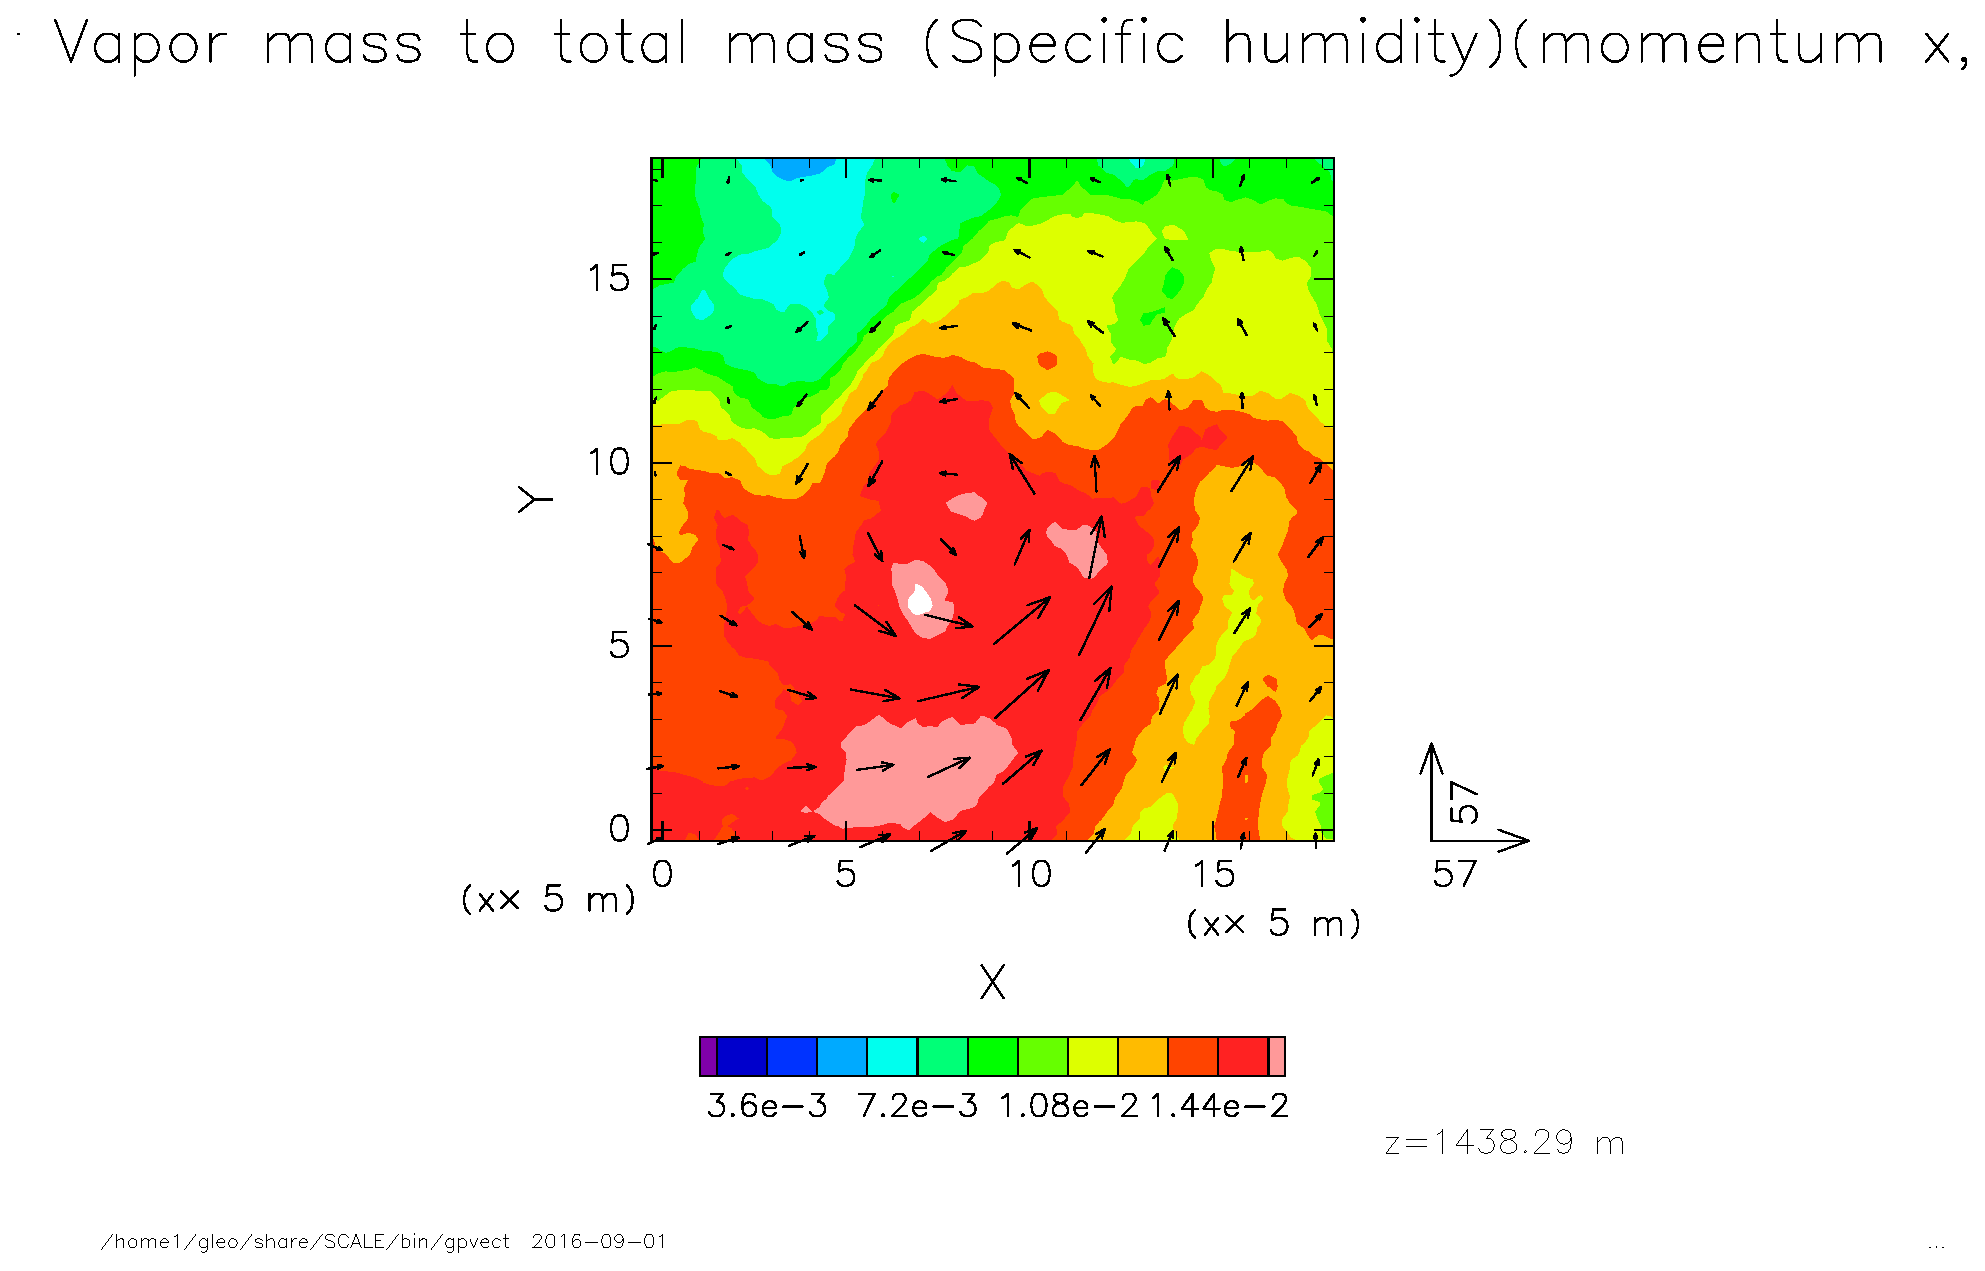
\includegraphics[width=0.9\hsize]{./figure/real_init_qv-momxy.eps}\\
  \caption{Initial field at z=1500m for the tutorial experiment. 
    The color indicates relative humidity and the vector horizontal momentum flux.}
  \label{fig:init}
\end{center}
\end{figure}

%-------------------------------------------------------%
\section{シミュレーションの実行:run} \label{sec:tutrial_real_run}
%-------------------------------------------------------%
\subsubsection{run.confの準備}
\verb|run|ディレクトリへ移動する。
\begin{verbatim}
 $ cd ${Tutorial_DIR}/real/experiment/run
\end{verbatim}
%
このディレクトリの中には、\verb|run.d01.conf|という名前の
設定ファイルが準備されており、
チュートリアル用の設定(表\ref{tab:grids}に合わせて設定されている。
他に\verb|run.launch.conf|というファイルも存在するが、ここでは使用しない。

モデル本体の実行には
事前に作成した地形データや初期値・境界値データを利用する。
これらのファイルの指定は、
\verb|run.d01.conf|の下記部分で設定している。\\

\noindent {\gt
\ovalbox{
\begin{tabularx}{150mm}{l}
\verb|&PARAM_TOPO| \\
\verb|   TOPO_IN_BASENAME = "../pp/topo_d01",| \\
\verb|/| \\
 \\
\verb|&PARAM_LANDUSE| \\
\verb|   LANDUSE_IN_BASENAME  = "../pp/landuse_d01",| \\
\verb|/| \\
 \\
\verb|&PARAM_RESTART| \\
\verb| RESTART_OUTPUT       = .true., |\\
\verb| RESTART_OUT_BASENAME = "restart_d01",|\\
\verb| RESTART_IN_BASENAME  = "../init/init_d01_20070714-180000.000",|\\
\verb|/| \\
 \\
\verb|&PARAM_ATMOS_BOUNDARY| \\
\verb| ATMOS_BOUNDARY_TYPE           = "REAL",                |\\
\verb| ATMOS_BOUNDARY_IN_BASENAME    = "../init/boundary_d01",|\\
\verb| ATMOS_BOUNDARY_START_DATE     = 2007, 7, 14, 18, 0, 0, |\\
\verb| ATMOS_BOUNDARY_UPDATE_DT      = 21600.0,               |\\
\verb| ATMOS_BOUNDARY_USE_DENS       = .true.,     |\\
\verb| ATMOS_BOUNDARY_USE_QHYD       = .false.,    |\\
\verb| ATMOS_BOUNDARY_ALPHAFACT_DENS = 1.0,        |\\
\verb| ATMOS_BOUNDARY_LINEAR_H       = .false.,    |\\
\verb| ATMOS_BOUNDARY_EXP_H          = 2.0,        |\\
\verb|/| \\
\end{tabularx}
}}\\


\verb|run.d01.conf|の中で、
時間積分に関する設定は\namelist{PARAM_TIME}において設定する。
初期時刻は、\nmitem{TIME_STARTDATE}にUTCで指定する。
チュートリアルでは、2007年7月14日18時UTCに設定している。
積分時間は、\nmitem{TIME_DURATION}で与える。
物理過程に対する時間ステップは、
それぞれの物理スキーム毎に設定できる。\\

\noindent {\gt\small
\ovalbox{
\begin{tabularx}{150mm}{ll}
\verb|&PARAM_TIME| & \\
\verb| TIME_STARTDATE         = 2007, 7, 14, 18, 0, 0,| & ← 時間積分を開始する時刻 \\
\verb| TIME_STARTMS           = 0.D0,  | &\\
\verb| TIME_DURATION          = 6.0D0, | & ← 積分期間 \\
\verb| TIME_DURATION_UNIT     = "HOUR",| & ← \verb|TIME_DURATION|の単位\\
\verb| TIME_DT                = 90.0D0,| & ← トレーサー移流計算の時間ステップ\\
\verb| TIME_DT_UNIT           = "SEC", | & ← \verb|TIME_DT|の単位\\
\verb| TIME_DT_ATMOS_DYN      = 45.0D0,| & ← トレーサー移流計算以外の力学過程の時間ステップ\\
\verb| TIME_DT_ATMOS_DYN_UNIT = "SEC", | & ← \verb|TIME_DT_ATMOS_DYN|の単位\\
 \\
\verb|   ..... 略 .....              | & \\
 \\
\verb|/| &\\
\end{tabularx}
}}\\


計算結果の出力に関する設定は、\nmitem{PARAM_HISTORY}で行う。\\

\noindent {\gt
\ovalbox{
\begin{tabularx}{150mm}{ll}
\verb|&PARAM_HISTORY| & \\
\verb|   HISTORY_DEFAULT_BASENAME  = "history_d01",| & ← 出力するファイル名\\
\verb|   HISTORY_DEFAULT_TINTERVAL = 3600.D0,      | & ← 出力時間間隔\\
\verb|   HISTORY_DEFAULT_TUNIT     = "SEC",        | & ← 出力時間間隔の単位\\
\verb|   HISTORY_DEFAULT_TAVERAGE  = .false.,      | & \\
\verb|   HISTORY_DEFAULT_DATATYPE  = "REAL4",      | & \\
\verb|   HISTORY_DEFAULT_ZCOORD    = "model",      | & ← 鉛直内挿は適用しない\\
\verb|   HISTORY_OUTPUT_STEP0      = .true.,       | & ← 初期時刻(t=0)の値を出力するかどうか\\
\verb|/| \\
\end{tabularx}
}}\\

上記の設定に従って、下記の\nmitem{HISTITEM}に列挙した変数を出力する。
必要があれば、\nmitem{HISTITEM}においてオプション変数を加えることで、変数毎に出力間隔を変更できる。
また、瞬間値の代わりに平均値を出力することも可能である。
これらの詳細は、\ref{sec:output}を参照されたい。\\

\noindent {{\gt
\ovalbox{
\begin{tabularx}{150mm}{ll}
\verb|&HISTITEM item="MSLP" /|        & 海面更正気圧 \\
\verb|&HISTITEM item="PREC" /|        & 降水強度 (2次元) \\
\verb|&HISTITEM item="OLR"  /|        & 外向き赤外放射(2次元) \\
\verb|&HISTITEM item="U10" / |        & 地表10mでのX方向水平速度成分(2次元) \\
\verb|&HISTITEM item="V10" / |        & 地表10mでのY方向水平速度成分(2次元) \\
\verb|&HISTITEM item="T2"  / |        & 地表2mでの温度 (2次元) \\
\verb|&HISTITEM item="Q2"  / |        &  地表2mでの水蒸気比湿 (2次元) \\
\verb|&HISTITEM item="SFC_PRES"   /|   & 地表気圧 (2次元) \\
\verb|&HISTITEM item="SFC_TEMP"   /|   & バルクの地表面温度 (2次元) \\
\verb|&HISTITEM item="DENS" /|        & 密度 (3次元) \\
\verb|&HISTITEM item="QV"   /|        & 水蒸気比湿 (3次元) \\
\verb|&HISTITEM item="QHYD" /|        & 全凝結物の全質量に対する比 (3次元) \\
\verb|&HISTITEM item="PRES" /|        & 圧力 (3次元) \\
\verb|&HISTITEM item="U"    /|        & X方向水平速度成分 (3次元) \\
\verb|&HISTITEM item="V"    /|        & Y方向水平速度成分 (3次元) \\
\verb|&HISTITEM item="T"    /|        & 温度 (3次元) \\
\verb|&HISTITEM item="W"    /|        & 鉛直方向速度成分 (3次元) \\
\verb|&HISTITEM item="Uabs" /|        & 風速 (3次元) \\
\verb|&HISTITEM item="PT"   /|        & 温位 (3次元) \\
\verb|&HISTITEM item="RH"   /|        & 相対湿度 (3次元) \\
\end{tabularx}
}}}\\

力学過程や物理過程に対するスキームとして他のスキームを用いたいときには、
力学過程に関しては\namelist{&PARAM_ATMOS_DYN}
物理過程に関しては\namelist{PARAM_ATMOS,PARAM_OCEAN,PARAM_LAND,PARAM_URBAN}で設定すれば良い。
詳細な内容については、第\ref{sec:atmos_dyn}節、\ref{sec:basic_usel_physics}節を参照されたい。

%
\subsubsection{シミュレーションの実行}

実行に必要なファイルは下記であり、これらはあらかじめ用意されている。
\begin{alltt}
 $ ls
    MIPAS  PARAG.29  PARAPC.29  VARDATA.RM29  cira.nc
                                  : 放射スキーム用のパラメータファイル
    run.d01.conf      : 設定ファイル
    param.bucket.conf : 陸面スキーム用のパラメータファイル
    scale-rm          : \scalerm の実行バイナリ
    run.launch.conf   : ネスティング計算用のlaunchファイル
                       (チュートリアルでは使用しない)
\end{alltt}
%
準備が整ったら、4-MPI並列により\scalerm を実行する。
\begin{verbatim}
  $ mpirun -n 4 ./scale-rm run.d01.conf >& log &
\end{verbatim}


実行が完了するまでには、ある程度時間を要する(推奨環境では10〜20分程度かかる)。
そのため、上記のように標準出力をファイルへ書き出すようにして
バックグラウンドで実行すると便利である。
計算が進みながら、途中経過のログは\verb|"LOG_d01.pe000000"|に出力される。
ジョブが正常に終了すると、\verb|"LOG_d01.pe000000"|の最後に\\

\noindent {\small {\gt
\fbox{
\begin{tabularx}{150mm}{l}
 +++++ finalize MPI...\\
 +++++ MPI is peacefully finalized\\
\end{tabularx}
}}}\\

\noindent と出力され、下記のファイルが作成される。
\begin{verbatim}
 $ ls
  history_d01.pe000000.nc
  history_d01.pe000001.nc
  history_d01.pe000002.nc
  history_d01.pe000003.nc
\end{verbatim}
各ファイルのサイズは、約 34 MB である。
出力ファイル(\verb|history_d01.pe######.nc|)は、
MPI のプロセス数に応じて分割されている。
ここで、\verb|######|はMPIプロセス番号を表す。
これらのファイルには、\nmitem{HISTITEM}で指定した変数が出力されている。
ファイル形式は、気候・予報(CF)メタデータ規約に対応したNetCDFである。



%####################################################################################


\section{Quick look at simulation result: net2g} \label{sec:quicklook}
%####################################################################################

In this section, we explain how to use netcdf2grads. The program netcdf2grads (for short, net2g) merges the \netcdf files (\verb|history.**.nc|)\footnote{If ``gpview'' is installed, it can also be used for drawing. This tool is more suitable for quick check  because it is available without the conversion of history data.},  which are divided process by process, into a binary file in \grads format. The simulation results are also validated using the converted \grads binary data.

\subsubsection{Conversion to \grads binary}
%-----------------------------------------------------------------------------------
Use \verb|net2g| to convert \grads binary from the history file of \netcdf having divided every process.  Only a minimum of the procedures is explained here.  Refer to Section \ref{sec:net2g} for their detailed use.

First, move to the directory \verb|net2g|:
\begin{verbatim}
 $ cd ${Tutorial_DIR}/real/experiment/net2g
 $ ls
    net2g -> ../../../../../util/netcdf2grads_h/net2g
    net2g.2D.d01.conf
    net2g.3D.d01.conf
\end{verbatim}
There are some configuration files and a binary file in this directory.  The binary file is linked to the executable file compiled in Section \ref{sec:source_net2g}. As an example,  a procedure to convert the 2D variables MSLP and PREC to \grads format is explained here. We also explain how to extract the 3D variables U and V at 850 hPa, 500 hPa, and 200 hPa, and convert them into \grads format.  The configuration files for 2D and 3D variables  are prepared as files \verb|net2g.3D.d01.conf| and \verb|net2g.2D.d01.conf|, respectively. 
 
When \verb|net2g| is executed, the number of processes needs to be a divisor of the number of the processes used for the simulation. 
The number of processes is four here. Since \verb|net2g| cannot simultaneously convert 2D and 3D variables , they must be converted separately as follows:
\begin{verbatim}
 $ mpirun -n 4 ./net2g net2g.2D.d01.conf
 $ mpirun -n 4 ./net2g net2g.3D.d01.conf
\end{verbatim}
The conversion succeeds only if the following messages are found  in the standard output without an error message:
\msgbox{
\verb|+++ MPI COMM: Corrective Finalize| \\
}
The following files are also found. \verb|**.ctl| represents the ``ctl'' file for the XY grid system of \scalerm, \verb|**lccr.ctl| a ctl file for the drawing results on the latitude-longitude coordinates:
\begin{verbatim}
  MSLP_d01z-2d.ctl
  MSLP_d01z-2d.grd
  MSLP_d01z-2d_lccr.ctl
  PREC_d01z-2d.ctl
  PREC_d01z-2d.grd
  PREC_d01z-2d_lccr.ctl
  PRES_d01z-3d.ctl
  PRES_d01z-3d.grd
  PRES_d01z-3d_lccr.ctl
  U_d01z-3d.ctl
  U_d01z-3d.grd
  U_d01z-3d_lccr.ctl
  V_d01z-3d.ctl
  V_d01z-3d.grd
  V_d01z-3d_lccr.ctl
\end{verbatim}


\subsubsection{Validation of simulation result}
%-----------------------------------------------------------------------------------
Confirm the calculation results using a \grads script \verb|checkfig_real.gs|: 
\begin{verbatim}
 $ cp ../../data/checkfig_real.gs ./
 $ grads -blc checkfig_real.gs
\end{verbatim}
The following files are generated when the conversion is successfully finished. Note that the script changes accordingly when a warning appears. This is because the syntax is different according to the version of \grads.
\begin{verbatim}
  real_mslp.png
  real_prec.png
  real_wind.png
\end{verbatim}
If the calculation are successful, the same figures as Figs. \ref{fig:real_mslp}, \ref{fig:real_prec}, and \ref{fig:real_wind}  are obtained.

\begin{figure}[tbh]
\begin{center}
  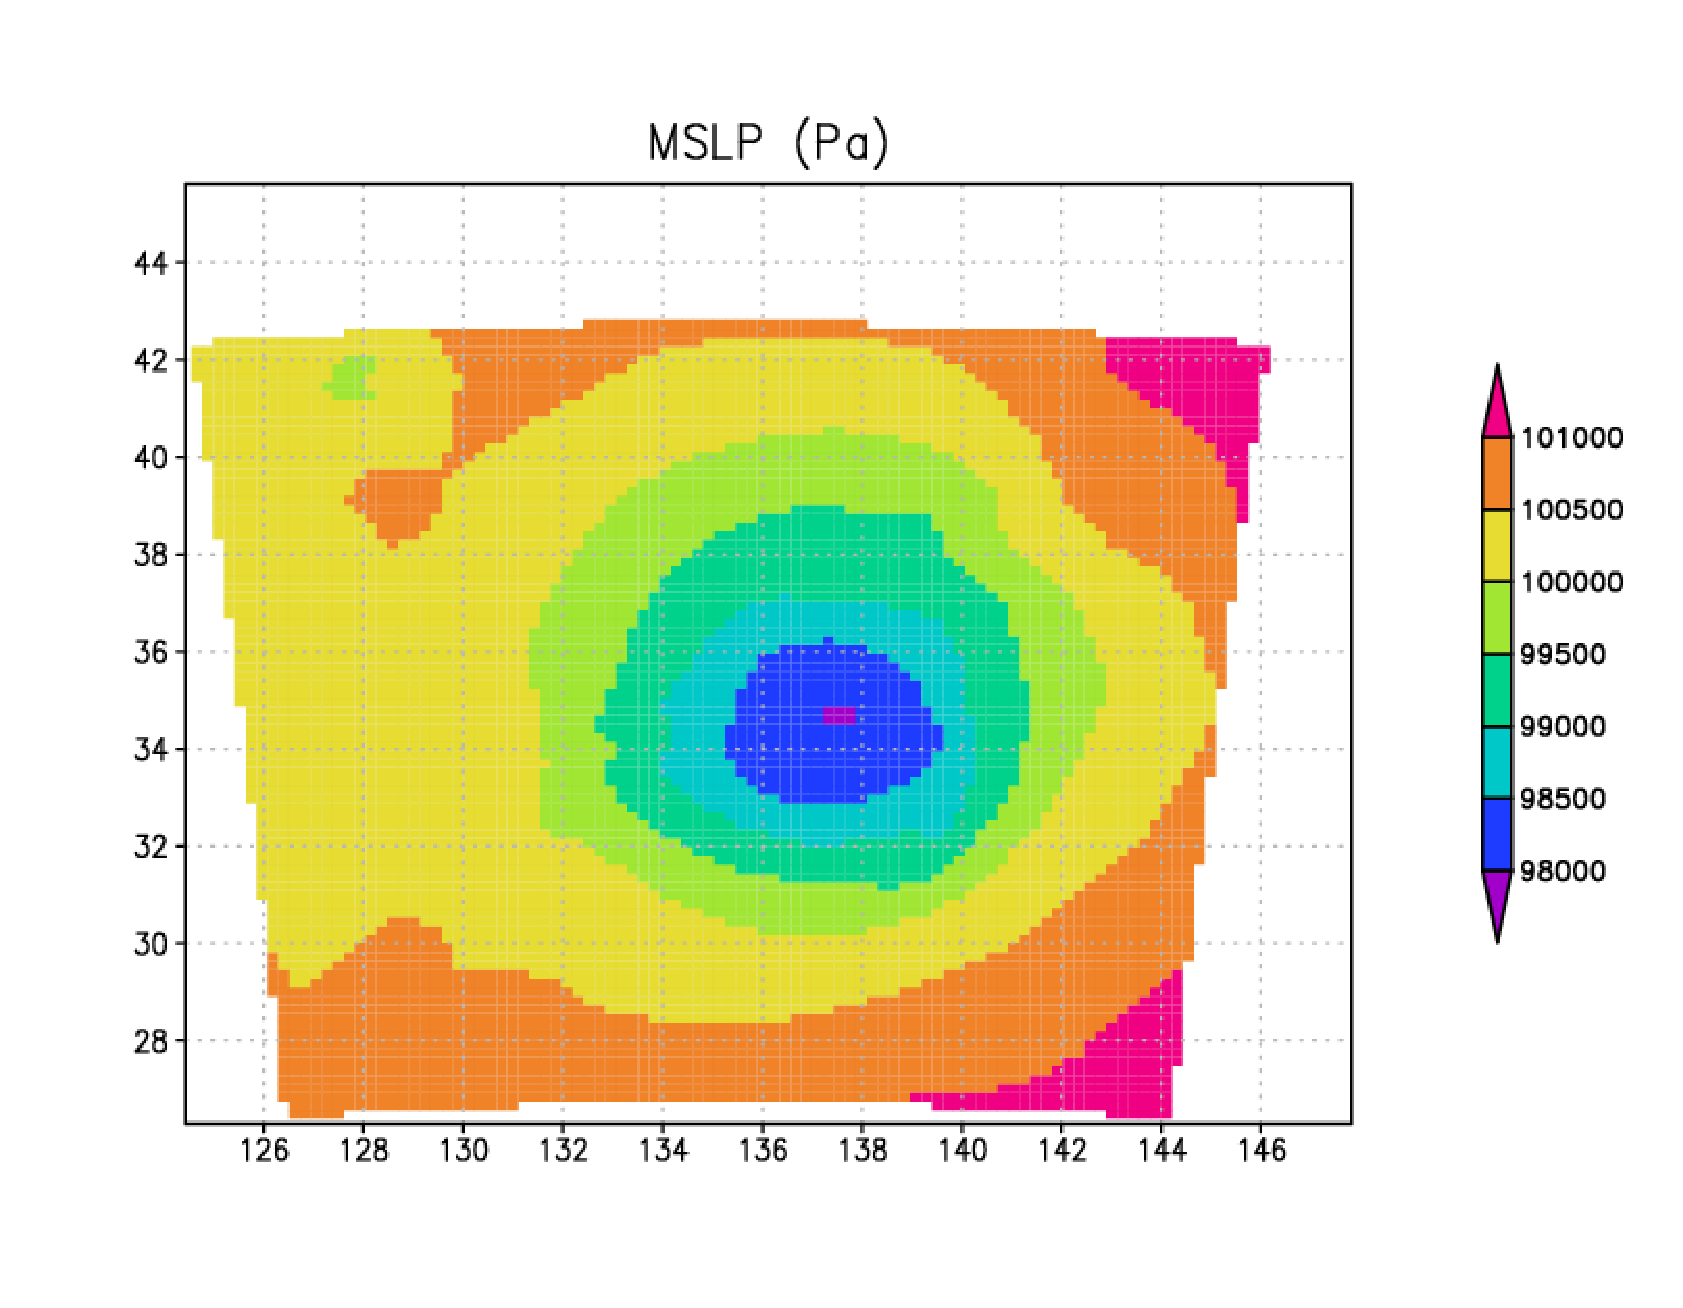
\includegraphics[width=0.55\hsize]{./figure/real_mslp.eps}\\
  \caption{Sea-level pressure after 6 hours}
  \label{fig:real_mslp}
\end{center}
\begin{center}
  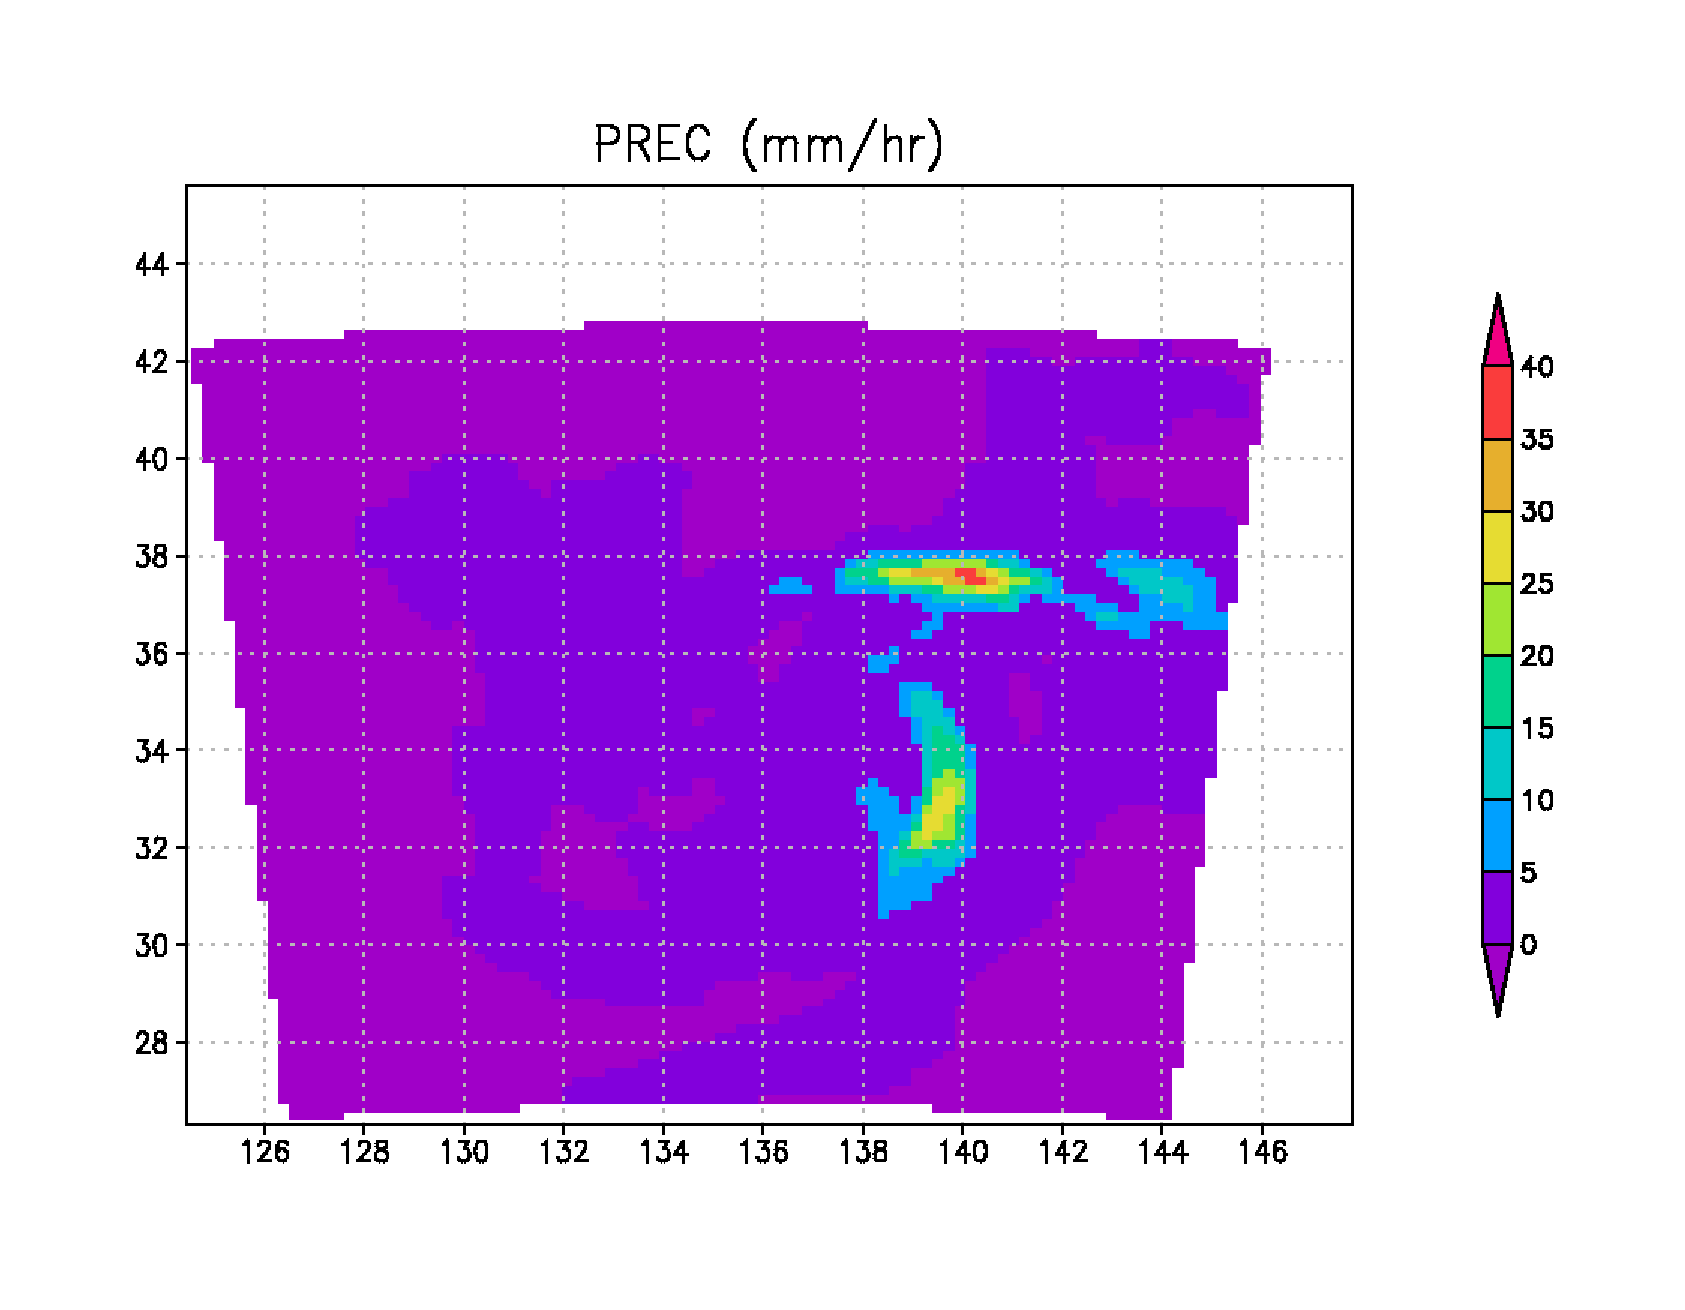
\includegraphics[width=0.55\hsize]{./figure/real_prec.eps}\\
  \caption{Precipitation flux after 6 hours}
  \label{fig:real_prec}
\end{center}
\begin{center}
  \includegraphics[width=0.55\hsize]{./figure/real_wind.eps}\\
  \caption{Wind velocity after 6 hours}
  \label{fig:real_wind}
\end{center}
\end{figure}



\chapter{Various settings} \label{chap:basic_usel}
%\section*{概要}

この章では、チュートリアルから発展して、基本的な様々な設定が出きるように、
各種設定を網羅的に記述している。
各節で閉じており、辞書代わりに使ってほしい。

%% {
%% \begin{center}
%% \begin{tabular}[h]{ll}\hline
%% \SecBasicDomainSetting & 第\ref{sec:domain} 節 \\
%%%%%% \SubsecDomainSetting & 第\ref{subsec:relation_dom_reso2} 節 \\
%% \SubsecMPIProcess & 第\ref{subsec:relation_dom_reso2} 節 \\
%% \SubsecGridNumSettng & 第\ref{subsec:relation_dom_reso3} 節 \\
%% \SubsecGridIntvSettng & 第\ref{subsec:gridinterv} 節 \\
%% \SecBasicBufferSetting & 第\ref{subsec:buffer} 節 \\
%% \SecBasicTopoSetting   & 第\ref{subsec:basic_usel_topo} 節 \\
%% \SecBasicIntegrationSetting & 第\ref{sec:timeintiv} 節 \\
%% \SecBasicOutputSetting & 第\ref{sec:output} 節\\
%% \SecBasicDynamicsSetting & 第\ref{sec:atmos_dyn} 節 \\
%% \SubsecDynsolverSetting  & 第\ref{subsec:atmos_dyn_sover} 節 \\
%% \SubsecDynSchemeSetting & 第\ref{subsec:atmos_dyn_scheme} 節 \\
%% \SecBasicPhysicsSetting & 第\ref{sec:basic_usel_physics} 節 \\
%% \SubsecMicrophysicsSetting & 第\ref{subsec:basic_usel_microphys} 節 \\
%% \SubsecTurbulenceSetting & 第\ref{subsec:basic_usel_turbulence} 節 \\
%% \SubsecRadiationSetting & 第\ref{subsec:basic_usel_radiation} 節 \\
%% \SubsecSurfaceSetting & 第\ref{subsec:basic_usel_surface} 節 \\
%% \SubsecOceanSetting & 第\ref{subsecp:basic_usel_ocean} 節 \\
%% \SubsecLandSetting & 第\ref{subsec:basic_usel_land} 節 \\
%% \SubsecUrbanSetting & 第\ref{subsec:basic_usel_urban} 節 \\
%% \SecMakeconfTool & 第\ref{sec:basic_makeconf} 節 \\
%% \SecAdvanceMapprojectionSetting & 第\ref{subsec:adv_mapproj}節 \\
%% \SecAdvanceInputDataSetting & 第\ref{sec:adv_datainput}節\\
%% \SecAdvanceRestart & 第\ref{sec:restart}節 \\
%% \SecAdvancePostprosess & 第\ref{sec:net2g}節 \\
%% \SecAdvanceNesting & 第\ref{sec:nest_exp}節 \\
%% \SubsecOflineNesting & 第\ref{subsec:nest_offline}節\\
%% \SubsecOnlineNesting & 第\ref{subsec:nest_online}節\\
%% \SecAdvanceBulkjob & 第\ref{sec:bulkjob}節\\
%% \hline
%% \end{tabular}
%% \end{center}
%% }

%\section{対象計算領域の設定} \label{sec:domain}
\section{\SecBasicDomainSetting} \label{sec:domain}
%=======================================================================

%\Item{\SubsecRelationOfResoGridProcess}
各設定を行う前に、\scalerm での対象計算領域の格子点数とMPIプロセスの関係を整理しておく。
計算領域は、水平格子間隔と格子点数を指定することで決定されるようになっている。
図\ref{fig:domain}は、
計算領域、水平格子間隔、格子数、及びMPIプロセス数の関係を示している。
水平方向に2次元の領域分割を行うことで並列化がなされている。

これらは、\namelist{PARAM_INDEX}内の\nmitem{IMAX,JMAX}、
\namelist{PARAM_PRC}内の\nmitem{PRC_NUM_X,PRC_NUM_Y}で設定する。
%水平格子間隔については、\namelist{PARAM_GRID}内の\nmitem{DX,DY}で設定する。

ここで、注意すべきことは、「指定する格子点数は各プロセスが受け持つ値」であることである。
設定する格子数(\nmitem{IMAX, JMAX,KMAX})は、
1つのMPIプロセスが担当する格子点数を与える仕様となっている。
すなわち、計算領域は、
水平格子間隔、格子点数とともに各方向のMPIプロセス数を考慮して決定する必要がある。

図\ref{fig:domain}に示すように、
MPIプロセス数が$n$(=\verb|PRC_NUM_X|$\times$\verb|PRC_NUM_Y|)の時、
計算領域は、\XDIR に\nmitem{PRC_NUM_X}個、\YDIR に\nmitem{PRC_NUM_Y}個に分割される。
以上の関係から、計算領域全体のそれぞれの方向の格子点数および総格子点数は、
\begin{eqnarray}
&& 領域内{\XDIR} の格子数 = \left(\verb|IMAX| \times \verb|PRC_NUM_X|\right)
   \times (\verb|KMAX| )  \label{eq:xgridnum}\\
&& 領域内{\YDIR}の格子数 = \left(\verb|JMAX| \times \verb|PRC_NUM_Y|
   \times (\verb|KMAX|\right)  \label{eq:ygridnum}\\
&& 領域内の総格子数 = \left(\verb|IMAX| \times \verb|PRC_NUM_X|\right)
   \times (\verb|JMAX| \times \verb|PRC_NUM_Y|)
   \times (\verb|KMAX| )  \nonumber
\end{eqnarray}
の関係となる。
ここで、\nmitem{KMAX}は、鉛直方向の格子点数であり、
\namelist{PARAM_INDEX}内の項目で指定されている。
次節以降では、MPIプロセス数、格子数、格子間隔、
それぞれの設定方法について詳しく説明する。

\begin{figure}[h]
\begin{center}
  \includegraphics[width=0.8\hsize]{./figure/domain_decomposition.eps}\\
  \caption{計算領域に対する、水平格子間隔(DX, DY)、1MPIプロセスあたりの格子数(IMAX, JMAX)、MPIプロセス数(PRC\_NUM\_X, PRC\_NUM\_Y)の関係。
水色領域は、ある1つのMPIプロセスが担当する領域。}
  \label{fig:domain}
\end{center}
\end{figure}

\subsection{\SubsecDomainSetting} \label{subsec:relation_dom_reso2}

前節で述べた関係が理解できれば、領域の設定は容易である。
すなわち、式(\ref{eq:xgridnum},\ref{eq:ygridnum})を使って、
\begin{eqnarray}
&& {\XDIR} の領域の長さ = {\XDIR} の格子点数 \times \verb|DX| \nonumber\\
&& {\YDIR}の領域の長さ = {\YDIR}の格子点数 \times \verb|DY| \nonumber
\end{eqnarray}
となる。ここで、\nmitem{DX,DY}は、後述するように
\namelist{PRAM_GRID}で指定されるものである。
逆算して、解像度と領域の大きさをを決めて、MPIプロセス数が決まると、
ローカルな領域の格子点数が決まる。

\subsection{\SubsecMPIProcess} \label{subsec:relation_dom_reso3}

MPIプロセス数は、設定ファイルの\namelist{PARAM_PRC}で指定する。
\scalerm の入出力ファイルは、MPIプロセス毎に分割されているため、
MPIプロセス数を変更すると分割ファイル数も必ず変わることになる。
従って、例えば、2-MPI並列用に作成した初期値ファイルは、
4-MPI並列のモデル実行には使用できない。
MPIプロセス数を変更するには、
\verb|pp_***.conf|、\verb|init_***.conf|、\verb|run_***.conf| の
すべてを編集・変更し、\verb|pp|, \verb|init| から行う必要がある。\\

\noindent {\small {\gt
\ovalbox{
\begin{tabularx}{140mm}{lX}
\verb|&PARAM_PRC| & \\
\verb| PRC_NUM_X       = 2,| & ; {\XDIR}(東西方向)のMPI並列分割数 \\
\verb| PRC_NUM_Y       = 1,| & ; {\YDIR}(南北方向)のMPI並列分割数 \\
\verb|/|\\
\end{tabularx}
}}}\\


全MPIプロセス数は、\verb|PRC_NUM_X| $\times$ \verb|PRC_NUM_Y|  となり、
上記の例では、\XDIR に2分割、\YDIR に1分割(分割なし)の
2-MPI並列ということになる。

実行時にMPIコマンドに指定するMPIプロセス数は、
この総MPIプロセス数を指定しなければならない。
この条件を満たさない場合は、下記のメッセージが
LOGファイルなどに出力されて計算は行われず、直ちに終了する。

\noindent {\small {\gt
\ovalbox{
\begin{tabularx}{140mm}{l}
\verb|xxx total number of node does not match that requested. Check!| \\
\end{tabularx}
}}}\\





\subsection{\SubsecGridNumSettng} \label{subsec:relation_dom_reso4}
%-----------------------------------------------------------------------

格子数の設定は、設定ファイル(\verb|***.conf|)の\namelist{PARAM_INDEX}で行う。
以下で設定する水平格子数の値は、1つのMPIプロセス当たりの値であることに注意が必要である。\\

\noindent {\small {\gt
\ovalbox{
\begin{tabularx}{140mm}{lX}
\verb|&PARAM_INDEX| & \\
\verb| KMAX = 97,|  & 鉛直層数 \\
\verb| IMAX = 20,|  & プロセスあたりの{\XDIR} の格子点数 \\
\verb| JMAX = 25,|  & プロセスあたりの{\YDIR}の格子点数 \\
\verb|/|\\
\end{tabularx}
}}}\\



\subsection{\SubsecGridIntvSettng} \label{subsec:gridinterv}
%-----------------------------------------------------------------------
\scalerm では、水平方向に格子間隔を一定値で設定する。
鉛直方向には、均等間隔でも任意の格子点位置を直接指定することもできる。
以下で説明する
\textcolor{red}{\bf 格子間隔の設定は、pp\_***.conf、init\_***.conf、run\_***.confの
設定ファイルの間で一致させなければならないことに注意が必要である。}

~\\

%-----------------------------------------------------------------------&
第\ref{subsec:buffer}節で述べる緩和領域を覗き、
水平格子間隔は等間隔でしか設定できない。
鉛直格子間隔については、任意に定義することが可能である。
すべての方向について等間隔で設定する場合には、以下のように
設定ファイルの\namelist{PARAM_GRID}の\nmitem{DX,DY,DZ}に
それぞれ、東西、南北、鉛直方向の格子間隔を指定する。
単位はmである。

\noindent {\small {\gt
\ovalbox{
\begin{tabularx}{140mm}{lX}
\verb|&PARAM_GRID  | & \\
\verb| DX = 500.D0,| & ; {\XDIR}(東西方向)の格子間隔\\
\verb| DY = 500.D0,| & ; {\YDIR}(南北方向)の格子間隔\\
\verb| DZ = 500.D0,| & ; {\ZDIR}(鉛直方向)の格子間隔\\
\verb|/|\\
\end{tabularx}
}}}\\


以下に、鉛直方向での任意の格子点位置を指定する場合の設定を示す。
鉛直方向は、ローレンツ格子を採用しており、
速度成分定義格子点とスカラー定義格子点が半格子分ずれた食い違い格子にになっている。
ここでは、スカラー量を定義している格子点をセンターポイントと呼び、
半格子ズレた格子点をフェイスポイントと呼ぶ(図\ref{fig:scale_grid}参照)。

直接格子点の位置を指定する場合は、フェイスポイントの位置を
\namelist{PARAM_GRID}の中の\nmitem{FZ(:)}で配列として与えればよい。
\footnote{指定の際には、シミュレーションの計算精度
(モデルのコンパイル時に指定した浮動小数点の精度。デフォルトでは倍精度)を用いることが望ましい。}
また、\nmitem{FZ(:)}で指定する値の数は、鉛直層数
(\namelist{PARAM_INDEX}の\nmitem{KMAX})と一致させる必要がある。
例として理想実験のチュートリアルのrun.confファイル
( run\_R20kmDX500m.conf )を下記に示す。

\noindent {\small {\gt
\ovalbox{
\begin{tabularx}{140mm}{lX}
\verb|&PARAM_GRID|     & \\
\verb| DX = 500.D0,|   & {\XDIR} の格子間隔(等間隔)[m]\\
\verb| DY = 500.D0,|   & {\YDIR}の格子間隔(等間隔)[m]\\
\verb| FZ(:) = |       & {\ZDIR}のフェイスポイントの位置[m] \\
\verb|    80.000000000000000      ,| & \\
\verb|    168.00000190734863      ,| & \\
\verb|    264.80000610351567      ,| & \\
\verb|     〜 中略 〜|           & \\
\verb|    14910.428862936289      ,| & \\
\verb|    15517.262523292475      ,| & \\
\verb|    16215.121232702089      ,| & \\
\verb|    17017.658748523147      ,| & \\
\verb|    17940.576891717363      ,| & \\
\verb|    19001.932756390710      ,| & \\
\verb|    20222.492000765058      ,| & \\
\verb| BUFFER_DZ = 5000.D0,|          & 第\ref{subsec:buffer}節参照\\
\verb| BUFFFACT  =   1.0D0,|          & 第\ref{subsec:buffer}節参照\\
\verb|/|\\
\end{tabularx}
}}}\\


\begin{figure}[tb]
\begin{center}
  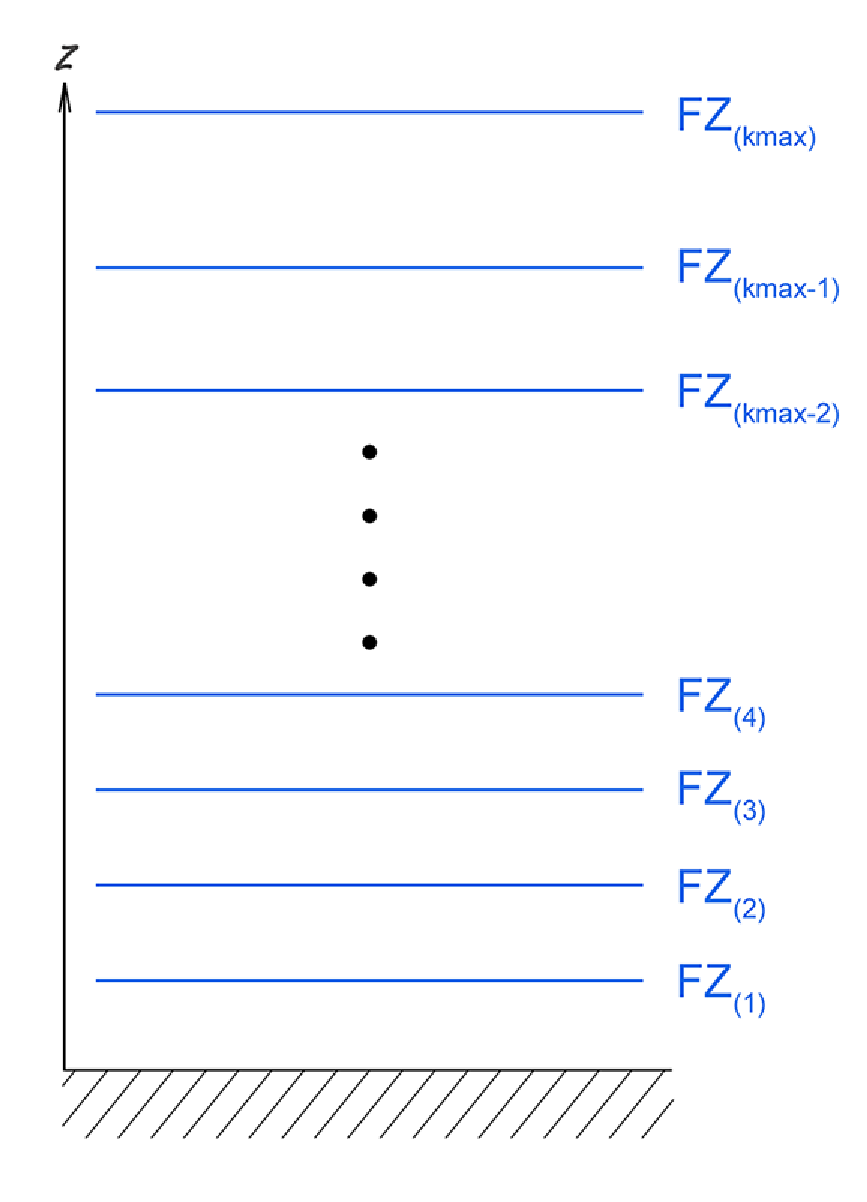
\includegraphics[width=0.4\hsize]{./figure/verticalface.eps}\\
  \caption{\scalerm の鉛直格子の定義点。\namelist{PARAM_GRID}で\nmitem{FZ}を指定する時は、ハロを除いた計算領域下端の格子から$k=1$として与える。}
  \label{fig:scale_grid}
\end{center}
\end{figure}
なお、これらの指定では、
標高0mでの格子点として設定され、標高を持つ位置では山岳に沿った座標系によって適切に処理される。


格子点位置は任意に設定できるが、場合によっては計算不安定につながる。
鉛直層の設定については、作成をサポートするツールが、\texttt{scale-\version/scale-rm/util/makevgrid/}
ディレクトリの中に`make\_vgrid.f90''というFortranプログラムと
いくつかのサンプルnamelistが用意されているので、参考にされたい。
ツールをコンパイルして実行すれば直ちに設定ファイルに貼り付けて使用できる
\nmitem{FZ(:)}の値が作成される。

\subsection{\SecAdvanceMapprojectionSetting} \label{subsec:adv_mapproj}
%------------------------------------------------------
\scalerm では、まず実距離に基づいた格子点が配置され、その格子点位置と緯度経度基準点の情報を元に、
それぞれの投影法を用いた際の各格子点での緯度・経度座標が計算される。
緯度・経度情報は、すべてのSCALEのNetCDF形式の出力ファイルに含まれている。\\
計算領域の位置と投影法は、設定ファイルの\nmitem{PARAM_MAPPROJ}の項目を編集することで設定できる。
\textcolor{red}{\bf この設定も、pp\_***.conf、init\_***.conf、run\_***.confの設定ファイルの間で
必ず一致させなければならない。}はじめに下記の例をもとに説明する。\\

\noindent {\small {\gt
\ovalbox{
\begin{tabularx}{140mm}{l}
\verb|&PARAM_MAPPROJ| \\
\verb| MPRJ_basepoint_lon = 138.727778D0,| \\
\verb| MPRJ_basepoint_lat = 35.360556D0,| \\
\verb| MPRJ_type          = 'MER',| \\
\verb|/| \\
\end{tabularx}
}}}\\

\begin{table}[b]
\begin{center}
\caption{SCALEで選択できる地図投影法}
\begin{tabularx}{150mm}{|l|X|} \hline
 \rowcolor[gray]{0.9} \verb|MPRJ_type| & 地図投影法 \\ \hline
 \verb|NONE| & 地図投影なし(理想実験用)、デフォルト \\ \hline
 \verb|LC|   & ランベルト正角円錐図法              \\ \hline
 \verb|PS|   & ポーラーステレオ図法                \\ \hline
 \verb|MER|  & メルカトル図法                     \\ \hline
 \verb|EC|   & 正距円筒図法                       \\ \hline
\end{tabularx}
\label{tab:map_proj}
\end{center}
\end{table}

\noindent
まず\nmitem{MPRJ_basepoint_lat}と\nmitem{MPRJ_basepoint_lon}は、
計算領域の中心の緯度・経度を表す。
SCALE-RMでは、北緯を正、南緯を負の値として表現し、
経度は0度を起点に右回りで表現するため、
この設定例では計算領域の
中心が北緯35.360556度、東経138.727778度に位置することになる。
この場所を中心に指定された大きさで、計算領域が設定される。\\
\nmitem{MPRJ_type}は、地図投影法の種類を表しており、\verb|MER|はメルカトル図法を意味する。
\scalerm で現在選択できる地図投影法とその指定文字列は表\ref{tab:map_proj}のとおりである。
メルカトル図法を用いた場合、投射する円筒に接する基準緯線は\nmitem{MPRJ_M_lat}で任意の値に設定する。
通常、基準緯線は赤道にとることが多いが、基準緯線に近いほど歪みが少なく正確に記述できるので、
\nmitem{MPRJ_M_lat}を指定しない場合は\nmitem{MPRJ_basepoint_lat}が基準緯線として用いられる。

\proofcomment{\nmitem{MPRJ_basepoint_lat}と\nmitem{MPRJ_M_lat}の使い分けの説明が不足しています。
記述してください.(八代)しました。}

投影法の中でも利用頻度が高いランベルト正角円錐図法の設定について以下に説明する。
ここでは、現実大気実験チュートリアルで使用した\verb|run.conf|ファイルを例に挙げる。\\

{\small {\gt
\ovalbox{
\begin{tabularx}{140mm}{l}
\verb|&PARAM_MAPPROJ| \\
\verb| MPRJ_basepoint_lon = 135.220404D0,| \\
\verb| MPRJ_basepoint_lat = 34.653396D0,| \\
\verb| MPRJ_type          = 'LC',| \\
\verb| MPRJ_LC_lat1       =  30.00D0,| \\
\verb| MPRJ_LC_lat2       =  40.00D0,| \\
\verb|/| \\
\end{tabularx}
}}}\\

\noindent
\scalerm では、2標準緯線型の投影方法を採用している。
両標準緯線に挟まれた領域では、
緯線・経線の長さの比が地球楕円体面上における長さの比と近くなるように調節される。
南側、北側の標準緯線はそれぞれ\nmitem{MPRJ_LC_lat1}と\nmitem{MPRJ_LC_lat2}で設定する。
値の単位はdegreeである。

さらに下記のように\nmitem{MPRJ_basepoint_x}と\nmitem{MPRJ_basepoint_y}という変数を用いることで、
地図投影中心と計算領域中心をずらすことができる。\\~\\

{\small {\gt
\ovalbox{
\begin{tabularx}{140mm}{l}
\verb|&PARAM_MAPPROJ| \\
\verb| MPRJ_basepoint_lon = 135.220404D0,| \\
\verb| MPRJ_basepoint_lat = 34.653396D0,| \\
\verb| MPRJ_basepoint_x   = 100.0D0,| \\
\verb| MPRJ_basepoint_y   = 100.0D0,| \\
\verb| MPRJ_type          = 'LC',| \\
\verb| MPRJ_LC_lat1       =  30.00D0,| \\
\verb| MPRJ_LC_lat2       =  40.00D0,| \\
\verb|/| \\
\end{tabularx}
}}}\\~\\

\noindent
\nmitem{MPRJ_basepoint_x}と\nmitem{MPRJ_basepoint_y}は、地図投影中心の位置を、
計算領域の南西端(左下角)からの距離で指定するパラメータで、単位はメートルである。
これらを指定しない場合、地図投影中心は計算領域中心に設定される。
地図投影中心を指定しない場合とした場合を比較したものを図\ref{fig:map_lc}に示す。
図\ref{fig:map_lc}aは、デフォルト設定で地図投影中心と計算領域中心が一致している場合、
図\ref{fig:map_lc}bは、地図投影中心をずらすよう指定した場合の関係を表している。
図\ref{fig:map_lc}bでは計算領域の南西端から
\nmitem{MPRJ_basepoint_x}と\nmitem{MPRJ_basepoint_y}で指定した距離だけ離れた位置に投影中心が設定される。

\begin{figure}[t]
\begin{center}
  \includegraphics[width=0.8\hsize]{./figure/LC_latlon_xy.eps}\\
  \caption{投影中心と計算領域の関係:(a)はデフォルト設定の場合、(b)は投影中心の位置を計算領域中心からずらした場合。
  赤線の矩形が計算領域を表す。}
  \label{fig:map_lc}
\end{center}
\end{figure}

\subsection{\SecBasicBufferSetting} \label{subsec:buffer}
%-----------------------------------------------------------------------
モデル最上層では意図しない重力波の反射が起こる。
また、側面境界では現実大気実験を行う際に境界条件と対象領域の間に値の不一致が起こる。
これを回避するため、「緩和領域」を設ける。
\scalerm では計算領域の境界のすぐ内側に緩和領域を設定することができる。
緩和領域の格子では、指定された値(境界値データ、親領域のデータなど)に対して
ある時定数で緩和される。以下これをナッジングと呼ぶ(上層における緩和はレイリーダンピングと呼ばれることが多い)。
緩和領域の幅は、設定ファイルの\namelist{PARAM_GRID}の中で設定する。
以下に例を示す。
設定はすべての設定ファイルにおいて共通していなければならない。\\

\noindent {\small {\gt
\ovalbox{
\begin{tabularx}{150mm}{lX}
\verb|&PARAM_GRID  |            & \\
 \verb|BUFFER_DZ = 5000.D0,   | & ; {\ZDIR}(モデルトップから下向き方向)の緩和領域の幅 [m]\\
 \verb|BUFFER_DX = 300000.D0, | & ; {\XDIR} (東西方向)の緩和領域の幅 [m]\\
 \verb|BUFFER_DY = 300000.D0, | & ; {\YDIR}(南北方向)の緩和領域の幅 [m]\\
 \verb|BUFFFACT  = 1.D0,      | & ; 緩和領域内の格子間隔に対するストレッチ係数(デフォルトは1.0)\\
\verb|/|\\
\end{tabularx}
}}}\\

水平方向には東西南北の四方境界に緩和領域が設定されるが、
鉛直方向には計算領域の上端にのみ緩和領域が設定され、下端には設定されない。
%
緩和領域は、計算領域内に設定されるため、
ナッジングの影響を受けない領域(緩和領域を除いた範囲)は
計算領域よりも狭くなることに注意が必要である。

\subsubsection{緩和領域の格子間隔をストレッチさせる}

緩和領域の格子間隔は、基本的に
\namelist{PARAM_GRID}の中の\nmitem{DX, DY, DZ}で指定した通りであるが、
\nmitem{BUFFFACT}に1以上の値を設定することで、ストレッチさせることも可能である。
ただし、格子間隔を等間隔で指定した場合、
この\nmitem{BUFFFACT}の設定は、X, Y, {\ZDIR}すべてに適用される。
それぞれの方向に別々に設定したい場合は、\nmitem{BUFFFACT_X}, \nmitem{BUFFFACT_Y}, \nmitem{BUFFFACT_Z}を指定する。
{\ZDIR}の層レベルを任意の格子点位置に指定する場合、
すなわち、\nmitem{FZ(:)}を与える場合(第\ref{subsec:gridinterv}節参照のこと)にはストレッチの設定は適用されない。

緩和領域内の格子間隔 (\verb|BDX|) は次の通り決定される。
\begin{eqnarray}
 \verb|BDX(|n\verb|)| &=& \verb|DX| \times \verb|BUFFFACT|^n \nonumber
\end{eqnarray}
ここで、$n$は緩和領域内の格子点番号を表し、計算領域の内側から外側へ向かって番号が振られる。
緩和領域の格子間隔は、
\nmitem{BUFFFACT=1.0}ならば内部領域と同じであり、
\nmitem{BUFFFACT=1.2}ならば内側から外側(境界)に向かって1.2倍の割合で広がっていく。
\nmitem{BUFFFACT}はいくつに設定しても良いが、計算の安定性を考慮すると 1.0から1.2 が推奨である。

緩和領域の格子数 \verb|ibuff|は、
\begin{eqnarray}
\sum_{n=1}^{\verb|ibuff|} \verb|BDX|(n) \ge \nmitemeq{BUFFER_DX} \nonumber
\end{eqnarray}
の関係を満たす最小の整数で自動的に計算され、緩和領域の大きさ\verb|BUFFER|$_x$は、
\[
  \verb|BUFFER|_x = \nmitemeq{DX} \times \frac{ \nmitemeq{BUFFFACT}^{\texttt{\detokenize{ibuff}}-1 }}{ \nmitemeq{BUFFFACT}-1 }
\]
となる。
結局、緩和領域を除いた計算領域の大きさは、
\[
\nmitemeq{DX} \times ( \nmitemeq{IMAX} \times \nmitemeq{PRC_NUM_X} - 2 \times \verb|ibuff| )
\]
となる。
%
緩和領域の幅\nmitem{BUFFER_DX}が同じでも、
\nmitem{BUFFFACT}の値を大きくすると緩和領域に用意される格子数は少なくなる。
ここでは、{\XDIR} の説明をしたが、{\YDIR}、{\ZDIR}も同様である。
ただし、{\ZDIR} については下端には緩和領域が取られないため、緩和領域を除いた計算領域の大きさは
\[
\nmitemeq{DZ} \times ( \nmitemeq{KMAX} - \verb|kbuff| )
\]
となる。

\proofcomment{ここは何度よんでも理解がしにくいです。結局この設定によって、真の対象領域は、
  どこなのか?を図に書いて説明してください}
\replycomment{式を追加しました。図はヨッシーに発注しています。(西澤)}
\proofcomment{了解しました。絵の追加を待って、本件終了させます。(富田)}
\replycomment{図を追加しました(吉田)}


一般に、緩和領域の大きさ、緩和格子点の数については、解く問題により、明確な指標はない。
\scalerm では、鉛直方向(計算領域トップ)の緩和格子点は5点以上、
水平方向(側面境界付近)の緩和格子点は20〜40点程度を推奨している。
実験設定や事例によっては、さらに緩和格子点を増やしたり、
ストレッチ係数を用いて緩和領域を広げたり、
緩和の時定数を調整したりする必要があるだろう。
時定数とは、目標値との差が$1/e$になるまでの時間である。
緩和の時定数は、
\namelist{PARAM_ATMOS_BOUNDARY}の中の
\nmitem{ATMOS_BOUNDARY_taux,ATMOS_BOUNDARY_tauy,ATMOS_BOUNDARY_tauz}によって秒単位で設定する。
デフォルトの値は $10 \Delta t$ であり、これは、10タイムステップで$1/e$になることに相当する。
タイムステップについては、第\ref{sec:timeintiv}節を参照のこと。

\begin{figure}[t]
\begin{center}
  \includegraphics[width=0.8\hsize]{./figure/buffer_xz.eps}\\
  \caption{計算領域における緩和領域の配置:斜線部分が緩和領域を意味する。
  図はXZ断面だが、Y方向にも同一の配置である。}
  \label{fig:buff_xz}
\end{center}
\end{figure}


\subsection{\SecBasicTopoSetting} \label{subsec:basic_usel_topo}
%-----------------------------------------------------------------------

\scalerm では地形データに対しモデル下端の格子面を傾斜させて地形を表現する山岳に沿った座標系を採用している。
水平の最大格子間隔を$DX_{max}$[m]、鉛直の最小格子間隔を$DZ_{min}$[m]とすると、許容される最大の地形傾斜角度$\theta_{max}$[deg]は次の式で計算される。

\[ \theta_{max} = \arctan( \mathrm{RATIO} \times \mathrm{DZ_{min}}/\mathrm{DX_{max}} ) \times 180/\pi \]

\scalerm ではRATIOのデフォルト値を1.0に設定している。
RATIOの設定を、1.0よりも大きくすれば地形がより細かく、1.0よりも小さくすれば地形がより粗く表現される。
ただしRATIOを1.0よりも大きくした場合、計算が途中で破綻する危険性が高くなる。

地形の設定は、設定ファイルの\namelist{PARAM_CNVTOPO}の中で設定する。
以下に例を示す。\\

\noindent {\small {\gt
\ovalbox{
\begin{tabularx}{150mm}{lX}
\verb|&PARAM_CNVTOPO  |                  & \\
 \verb|CNVTOPO_name                  = "GTOPO30", | & ; 使用する地形データ名\\
 \verb|CNVTOPO_smooth_maxslope_ratio = 1.0,       | & ; DZのDXに対する比の倍率 \\
 \verb|CNVTOPO_smooth_local          = .true.,    | & ; 最大傾斜角度を超えた格子のみ平滑化を行うかどうか \\
 \verb|CNVTOPO_copyparent            = .false.,   | & ; 緩和領域に親ドメインの地形をコピーするかどうか \\
\verb|/|\\
\end{tabularx}
}}}\\


使用する地形データの名称を与え、地形データを読み込む。
\scalerm ではGTOPO30、または国土地理院による高精度地形データ(DEM50M)をサポートしている。

最大傾斜角度を超える傾斜角が与えられた地形データ内に検出された場合、
それを最大傾斜角度以下になるように、反復計算を用いて徐々に平滑化を実行する。
このとき、最大傾斜角度を超えた格子のみ平滑化を行うか、計算領域全体で行うかを選択することができる。
前者は、最大傾斜角度以内のシャープな地形構造を残すことができるので、細かな地形表現を望む場合に選択する。

上記の計算式で分かるように、許容される最大傾斜角度は空間解像度に応じて変わる。
一般的に、多段ネスティング計算を行う場合、
子ドメインのほうが空間解像度が細かいため、地形もシャープに表現される。
このとき、親ドメインと子ドメインの地形表現が異なるために、
子ドメインの緩和領域に挿入される親ドメインの大気データを外挿する必要が発生し、不整合を起こすことがある。
これを回避するために、
\nmitem{CNVTOPO_copyparent}を\verb|.true.|とすることで、親ドメインの地形を子ドメインの緩和領域にコピーすることができる。
親ドメインが存在しない場合は\nmitem{CNVTOPO_copyparent}を必ず\verb|.false.|に設定しなければならない。

\section{\SecMapprojectionSetting} \label{subsec:adv_mapproj}
%------------------------------------------------------
\scalerm では、格子点は実距離に基づいて配置される。
各格子点での緯度・経度の値は、基準位置の緯度経度を与えることによって、ある地図投影法から計算される。
格子の緯度・経度に関する情報は、SCALE が生成するNetCDF形式の全出力ファイルに含まれる。
計算領域の位置と地図投影法は、\nmitem{PARAM_MAPPROJECTION}で設定できる。
この設定は、\textcolor{blue}{\texttt{pp.conf}、\texttt{init.conf}、\texttt{run.conf}の設定ファイル間で一致させなければならない}。
上記の設定例を以下に示す。\\
\editboxtwo{
\verb|&PARAM_MAPPROJECTION| & \\
\verb| MAPPROJECTION_basepoint_lon = 138.727778D0,| & \\
\verb| MAPPROJECTION_basepoint_lat = 35.360556D0,|  & \\
\verb| MAPPROJECTION_type          = 'MER',|        & ; 表\ref{tab:map_proj}から選択.\\
\verb|/| & \\
}

\begin{table}[b]
\begin{center}
\caption{\scalerm で選択可能な地図投影法}
\begin{tabularx}{150mm}{|l|X|} \hline
 \rowcolor[gray]{0.9} \verb|MPRJ_type| & 地図投影法 \\ \hline
 \verb|NONE| & 地図投影なし(理想実験用)、デフォルト \\ \hline
 \verb|LC|   & ランベルト正角円錐図法              \\ \hline
 \verb|PS|   & ポーラーステレオ図法                \\ \hline
 \verb|MER|  & メルカトル図法                     \\ \hline
 \verb|EC|   & 正距円筒図法                       \\ \hline
\end{tabularx}
\label{tab:map_proj}
\end{center}
\end{table}

\noindent
\nmitem{MPRJ_basepoint_lat, MPRJ_basepoint_lon}は、
それぞれ基準点の緯度・経度である。
デフォルトの設定では、基準点は計算領域の中心である。
\scalerm では、北緯を正、南緯を負の値として表現し、
東経を正、西経を負の値として表現する。
経度は180度以上の値を用いて表現することができる。
上記の設定では、計算領域の中心が北緯35.360556度、東経138.727778度に設定される。
全計算領域は、指定された大きさでこの場所を中心にして配置される。

\nmitem{MAPPROJECTION_type}は地図投影法の種類を表しており、\verb|MER|はメルカトル図法を意味する。
表\ref{tab:map_proj}は、\scalerm で現在選択できる地図投影法を示している。
メルカトル図法の場合には、投射する円筒に接する基準緯線は\nmitem{MAPPROJECTION_M_lat}(単位は度)で設定する。
一般的に基準緯線は赤道にとられることが多い。
しかし、メルカトル図法は基準緯線に近いほど歪みが少なく正確であるので、
\scalerm では、\nmitem{MAPPROJECTION_M_lat}を陽に指定しなければ、
\nmitem{MAPPROJECTION_basepoint_lat}を基準緯線として用いる。

次に、地図投影法の中でも利用頻度が高い、ランベルト正角円錐図法の設定を以下で説明する。
以下の例は、現実大気実験チュートリアルで使用した\verb|run.d01.conf|ファイル内の記述と同じである。\\

{\small {\gt
\ovalbox{
\begin{tabularx}{150mm}{l}
\verb|&PARAM_MAPPROJECTION| \\
\verb| MAPROJECTION_basepoint_lon = 135.220404,| \\
\verb| MAPROJECTION_basepoint_lat = 34.653396,| \\
\verb| MAPROJECTION_type          = 'LC',| \\
\verb| MAPROJECTION_LC_lat1       =  30.0,| \\
\verb| MAPROJECTION_LC_lat2       =  40.0,| \\
\verb|/| \\
\end{tabularx}
}}}\\

\noindent
\scalerm では、2標準緯線型の投影方法を採用している。
南側、北側の標準緯線はそれぞれ\nmitem{MAPROJECTION_LC_lat1, MAPROJECTION_LC_lat2}(単位は[度])で指定する。
両標準緯線に挟まれた領域では、
緯線・経線の長さの比が地球楕円体面上における長さの比と近くなるように調節される。

さらに下記のように設定すれば、
基準点(\nmitem{MAPROJECTION_basepoint_x, MAPROJECTION_basepoint_y})を、
デフォルト設定である計算領域の中心からずらすことができる。\\~\\

{\small {\gt
\ovalbox{
\begin{tabularx}{150mm}{l}
\verb|&PARAM_MAPPROJ| \\
\verb| MPRJ_basepoint_lon = 135.220404,| \\
\verb| MPRJ_basepoint_lat = 34.653396,| \\
\verb| MPRJ_basepoint_x   = 100.0,| \\
\verb| MPRJ_basepoint_y   = 100.0,| \\
\verb| MPRJ_type          = 'LC',| \\
\verb| MPRJ_LC_lat1       = 30.0,| \\
\verb| MPRJ_LC_lat2       = 40.0,| \\
\verb|/| \\
\end{tabularx}
}}}\\~\\

\noindent
地図投影中心の位置は、計算領域の南西端(左下角)からの距離によって指定する。つまり、\\
\nmitem{MAPROJECTION_basepoint_x, MAPPROJECTION_basepoint_y}はそれぞれ、
\XDIR や \YDIR に対する左下角と基準位置の間の距離(単位は[m])である。
これらを指定しない場合、地図投影の中心は計算領域の中心に設定される。
図\ref{fig:map_lc}に、両方の場合における地図投影の中心と計算領域の関係を示す。
%図\ref{fig:map_lc}(a)は、デフォルト設定で地図投影中心と計算領域中心が一致している場合、
%図\ref{fig:map_lc}(b)は、地図投影中心をずらすよう指定した場合の関係を表している。
%図\ref{fig:map_lc}(b)では計算領域の南西端から
%\nmitem{MPRJ_basepoint_x, MPRJ_basepoint_y}で指定した距離だけ離れた位置に投影中心が設定される。

\begin{figure}[t]
\begin{center}
  \includegraphics[width=0.8\hsize]{./figure/LC_latlon_xy.eps}\\
  \caption{投影中心と計算領域の関係:(a)はデフォルト設定の場合、(b)は投影中心の位置を計算領域中心からずらした場合。
  赤線は計算領域の境界を表す。}
  \label{fig:map_lc}
\end{center}
\end{figure}

\section{\SecBasicTopoSetting} \label{subsec:basic_usel_topo}
%-----------------------------------------------------------------------

\scalerm では地形を表現するために、地形に沿った座標系を採用している。
この座標系では、最下層の格子の底面が標高に対して沿うように与えられる。
許容される最大の地形傾斜角度$\theta_{\max}$ [radian]は、次の式で計算する。
\[
  \theta_{\max} = \arctan( \mathrm{RATIO} \times \mathrm{DZ}/\mathrm{DX} )
\]
ここで、$\mathrm{DZ}$と$\mathrm{DX}$はそれぞれ、鉛直方向と水平方向の格子間隔である。
上記の計算式から分かるように、許容される最大傾斜角度は空間解像度に応じて変わる。
$\mathrm{RATIO}$が1.0よりも大きければ地形はより細かく表現され、1.0よりも小さければ粗く表現される。
$\mathrm{RATIO}$を非常に大きく設定した場合には、計算が途中で破綻する危険性が高くなることに注意が必要である。
\scalerm では$\mathrm{RATIO}$のデフォルト値は1.0に設定している。

\verb|scale-rm_pp|は、外部入力する標高データを{\scalelib}形式に変換するためのプログラムである。
詳細な設定は、設定ファイル\verb|pp.conf|の\namelist{PARAM_CNVTOPO}の中で行う。
以下に例を示す。\\

\editboxtwo{
\verb|&PARAM_CNVTOPO                               | & \\
\verb|CNVTOPO_UseGTOPO30            = .true.,      | & ; GTOPO30 データセットを用いるか? \\
\verb|CNVTOPO_UseDEM50M             = .false.,     | & ; DEM50M データセットを用いるか? \\
\verb|CNVTOPO_UseUSERFILE           = .false.,     | & ; ユーザ定義のデータセットを用いるか? \\
\verb|CNVTOPO_smooth_type           = 'LAPLACIAN', | & ; 平滑化のためのフィルタの種類 (OFF,LAPLACIAN,GAUSSIAN) \\
\verb|CNVTOPO_smooth_maxslope_ratio = 10.D0,       | & ; 許容する傾斜の$\mathrm{DZ}$/$\mathrm{DX}$に対する倍率 \\
\verb|CNVTOPO_smooth_maxslope       = -1.D0,       | & ; 許容する傾斜角の最大値 [deg] \\
\verb|CNVTOPO_smooth_local          = .true.,      | & ; 最大傾斜角度を超えた格子でのみ平滑化を続けるかどうか? \\
\verb|CNVTOPO_smooth_itelim         = 10000,       | & ; 平滑化の繰り返し回数の制限値 \\
\verb|CNVTOPO_smooth_hypdiff_niter  = 20,          | & ; 超粘性による平滑化の繰り返し回数 \\
\verb|CNVTOPO_interp_level          = 5,           | & ; 補間に用いる近隣の格子点数 \\
\verb|CNVTOPO_copy_parent           = .false.,     | & ; 子ドメインの緩和領域に親ドメインの地形をコピーするか? \\
\verb|/                                            | \\
}

\scalerm では地形データの入力として、国土地理院が提供する
GTOPO30 と DEM50M に対応している。
プログラム\verb|scale-rm_pp|によってユーザが準備した地形データを変換できる(第\ref{subsec:topo_userfile}節を参照)。
また、上記のデータセットを組み合わせることもできる。
\nmitem{CNVTOPO_UseGTOPO30}と\nmitem{CNVTOPO_UseDEM50M}の両方を
\verb|true|に設定した場合は、プログラムは以下のようにデータを作成する。

\begin{itemize}
 \item GTOPO30 のデータセットを計算領域の格子点に内挿する。
 \item DEM50M が対象とする領域は、DEM50M のデータセットを用いて内挿し、上書きする。
 \item 平滑化を適用する。
\end{itemize}

デフォルトでは、対象とする格子点の周辺にある、入力データの最寄りの5格子点が内挿に使われる。
使用する格子点数は\nmitem{CNVTOPO_interp_level}によって決定される。
地形のリグリッドにおいて、急な傾斜を含む標高を平滑化するためのフィルタとして、
ラプラシアンフィルタとガウスシアンフィルタの2種類が存在する。
これは\nmitem{CNVTOPO_smooth_type}で選択することができ、
デフォルトではラプラシアンフィルタが用いられる。
平滑化の操作において、傾斜角が最大許容角度$\theta_{\max}$を下回るまで、選択されたフィルタが適用される。
\nmitem{CNVTOPO_smooth_maxslope_ratio}を指定することによって、上記の$\mathrm{RATIO}$を直接設定できる。
または、度数で最大傾斜角を決める\nmitem{CNVTOPO_smooth_maxslope}を用いることができる。
平滑化の繰り返し回数の上限はデフォルトでは 10000 回であるが、\nmitem{CNVTOPO_smooth_itelim}を設定することで繰り返し回数を増やせる。
\nmitem{CNVTOPO_smooth_local}を\verb|.true.|に設定した場合は, 繰り返されるフィルタ操作は平滑化が完了していない格子点でのみ続けられる。

小さな空間スケールのノイズを取り除くために、付加的な超粘性を地形に適用する。
シミュレーションにおける数値的なノイズを減らすために、このフィルタリングを行うことを推奨する。
\nmitem{CNVTOPO_smooth_hypdiff_niter}に負の値を設定した場合は、このフィルタは適用されない。

\nmitem{CNVTOPO_copy_parent}は、ネスティング計算のための設定項目である。
一般的に、子ドメインは親ドメインよりも空間解像度が高いために、子ドメインの方が地形がより細かく表現される。
このとき、子ドメインの緩和領域における大気データと親ドメインにおける大気データの間の不整合によって、問題がしばしば起きる。
この問題を回避するために、\nmitem{CNVTOPO_copy_parent}を\verb|.true.|とすれば親ドメインの地形を子ドメインの緩和領域にコピーできる。
親ドメインが存在しない場合は\nmitem{CNVTOPO_copy_parent}を\verb|.false.|に設定しなければならない。
\nmitem{CNVTOPO_copy_parent}を利用する場合の設定は、第\ref{subsec:nest_topo}節で詳しく説明する。


\section{ユーザー定義の地形の準備} \label{subsec:topo_userfile}

\nmitem{CNVTOPO_UseUSERFILE}を\verb|.true.|に設定した場合は、プログラム\verb|scale-rm_pp|は \\
\namelist{PARAM_CNVTOPO_USERFILE}で指定したファイルの変換を行う.

入力データのタイプを\nmitem{USERFILE_TYPE}で指定する。
サポートされているタイプは ``GrADS'' と ``TILE'' である。

``GrADS''タイプを指定した場合、別途入力ファイルのデータ構造を記述するネームリストファイルが必要となる。
このネームリストファイルは\nmitem{USERFILE_GrADS_FILENAME}で指定する。
ネームリストファイルの詳細については、\ref{sec:datainput_grads}を参照のこと。
デフォルトでは、地形、緯度、経度データの変数名のデフォルト値はそれぞれ``topo'', ``lat'', ``lon''であるが、
異なる場合は、それぞれ\nmitem{USERFILE_GrADS_VARNAME}、\nmitem{USERFILE_GrADS_LATNAME}、\nmitem{USERFILE_GrADS_LONNAME}で指定することができる。


``TILE''タイプを指定した場合、カタログファイルが必要である。
カタログファイルには、それぞれのタイルデータファイルの名前およびそれぞれがカバーする領域についての情報が記述されている。
同じ形式である GTOPO30 や DEM50 のカタログファイルを参照するとよい。
以下はカタログファイルの例である。
\editboxtwo{
\verb|001 -90.0  0.0 -180.0   0.0 TILE_sw.grd| & ; 南緯90--0 西経180--0 の範囲, ファイル名 \verb|TILE_sw.grd| \\
\verb|002 -90.0  0.0    0.0 180.0 TILE_se.grd| & ; 南緯90--0 東経0--180 の範囲, ファイル名 \verb|TILE_se.grd| \\
\verb|003   0.0 90.0 -180.0   0.0 TILE_nw.grd| & ; 北緯0--90 西経180--0 の範囲, ファイル名 \verb|TILE_nw.grd| \\
\verb|004   0.0 00.0    0.0 180.0 TILE_ne.grd| & ; 北緯0--90 東経0--180 の範囲, ファイル名 \verb|TILE_ne.grd| \\
}
それぞれのタイルデータは \grads(direct access) 形式と同じ単純なバイナリ形式である。
以下は設定例である。
\editboxtwo{
\verb|&PARAM_CNVTOPO_USERFILE                     | & \\
\verb|USERFILE_CATALOGUE  = "catalogue.txt",      | & ; カタログファイルの名前 \\
\verb|USERFILE_DIR        = "./input_topo",       | & ; 入力ファイルがあるディレクトリのパス \\
\verb|USERFILE_DLAT       = 0.0083333333333333D0, | & ; 格子間隔 (緯度,degree) \\
\verb|USERFILE_DLON       = 0.0083333333333333D0, | & ; 格子間隔 (経度,degree) \\
\verb|USERFILE_DTYPE      = "INT2",               | & ; データの種類 (INT2,INT4,REAL4,REAL8) \\
\verb|USERFILE_yrevers    = .true.,               | & ; データは緯度方向に関して北から南へと格納されているか? \\
\verb|/                                           | \\
}
この例では、\verb|catalogue.txt|という名前のカタログファイルが、ティレクトリ\verb|./input_topo|に存在する。
値は2バイトの整数で格納されている。


\section{How to create initial and boundary data} \label{sec:adv_datainput}
%====================================================================================

\begin{table}[tbh]
\begin{center}
\caption{External input data supported in \scalelib}
\begin{tabularx}{150mm}{l|l|X} \hline
 \rowcolor[gray]{0.9} Data type   & \verb|FILETYPE_ORG|  & Note \\ \hline
 SCALE format   & \verb|SCALE-RM|     & Only history files are supported. The latitude-longitude catalog is needed. \\ \hline
 Binary format  & \verb|GrADS|        & Another namelist for data input is required.    \\ \hline
 WRF format     & \verb|WRF-ARW|      & Both ``wrfout''  and``wrfrst'' are supported.\\ \hline
\end{tabularx}
\label{tab:inputdata_format}
\end{center}
\end{table}

\scalerm can generate initial and boundary data by entering various types of external data, as shown in Table \ref{tab:inputdata_format}. The program \verb|scale-rm_init| converts external data into boundary and initial data by configuring the file \verb|init.conf|. The input data format is specified at \nmitem{FILETYPE_ORG} in \namelist{PARAM_MKINIT_REAL_***}. The SCALE format is mainly used for offline nesting. Refer to Section \ref{subsec:nest_offline} for details. The WRF data format is available; WRF model output data can be used directly. Note that the file should contain all data required for the generation of the boundary data of \scalerm. The ``binary format'' in this documentation is defined as binary data with single-precision floating points that FORTRAN can directly access. GRIB/GRIB2 data are available by converting them to binary format; this procedure is explained in Section \ref{sec:tutrial_real_data}. Other arbitrary data can also be used if it is converted into binary format.

%%%---------------------------------------------------------------------------------%%%%
\subsubsection{Input from binary format data} \label{sec:datainput_grads}

The input data format is specified in \namelist{PARAM_MKINIT_REAL_***} in the configuration file \verb|init.conf|
as follows:
\editbox{
\verb|&PARAM_RESTART|\\
\verb| RESTART_OUTPUT       = .true.,|\\
\verb| RESTART_OUT_BASENAME = "init_d01",|\\
\verb|/|\\
\\
\verb|&PARAM_MKINIT_REAL_ATMOS|\\
\verb| NUMBER_OF_FILES      = 2,|\\
\verb| FILETYPE_ORG         = "GrADS",|\\
\verb| BASENAME_ORG         = "namelist.grads_boundary.FNL.grib1",|\\
\verb| BASENAME_BOUNDARY    = "boundary_d01",|\\
\verb| BOUNDARY_UPDATE_DT   = 21600.0,|\\
\verb| PARENT_MP_TYPE       = 3,|\\
\verb| USE_FILE_DENSITY     = .false.,|\\
\verb|/|\\
\verb|&PARAM_MKINIT_REAL_OCEAN|\\
\verb| NUMBER_OF_FILES      = 2,|\\
\verb| FILETYPE_ORG         = "GrADS",|\\
\verb| BASENAME_ORG         = "namelist.grads_boundary.FNL.grib1",|\\
\verb| INTRP_OCEAN_SFC_TEMP = "mask",|\\
\verb| INTRP_OCEAN_TEMP     = "mask",|\\
\verb|/|\\
\verb|&PARAM_MKINIT_REAL_LAND|\\
\verb| NUMBER_OF_FILES      = 2,|\\
\verb| FILETYPE_ORG         = "GrADS",|\\
\verb| BASENAME_ORG         = "namelist.grads_boundary.FNL.grib1",|\\
\verb| USE_FILE_LANDWATER   = .true.,|\\
\verb| INTRP_LAND_TEMP      = "mask",|\\
\verb| INTRP_LAND_WATER     = "fill",|\\
\verb| INTRP_LAND_SFC_TEMP  = "fill",|\\
\verb|/|\\
}

If binary data is entered, \verb|"GrADS"| is given to \nmitem{FILETYPE_ORG}.
In \scalerm, the namelist file \verb|namelist.grads_boundary**|, which contains the file name and the structure of binary data, is prepared instead of the ``ctl'' file. Give its path at \nmitem{BASENAME_ORG}.

\nmitem{NUMBER_OF_FILES} is the number of input files.
In case of a single input file, prepare only file \verb|"filename.grd"|.
In the case of multiple input files, prepare the files numbered as \verb|"filename.XXXXX.grd"| in the forward direction.
The program \verb|scale-rm_init| reads these files enumerated from \verb|00000| to the given number \nmitem{NUMBER_OF_FILES}-1.
The header name of input files, i.e., \verb|"filename"|, is specified in the namelist file and explained later.

\nmitem{BOUNDARY_UPDATE_DT} is the time step of input data.
\nmitem{RESTART_OUT_BASENAME} in \namelist{PARAM_RESTART} is the header name of the initial file converted.
\nmitem{BASENAME_BOUNDARY} is the header name of the boundary files converted.

The above configurations are the common among \namelist{PARAM_MKINIT_REAL_ATMOS},\\ \namelist{PARAM_MKINIT_REAL_OCEAN}, and \namelist{PARAM_MKINIT_REAL_LAND}. Unless otherwise specified in\\
\namelist{PARAM_MKINIT_REAL_OCEAN} and \namelist{PARAM_MKINIT_REAL_LAND}, these information are inherited. 


\nmitem{USE_FILE_DENSITY} is an option in case of \verb|FILETYPE_ORG="SCALE-RM"|.
If binary data is selected, provide \verb|.false.| to \nmitem{USE_FILE_DENSITY}.
\nmitem{PARENT_MP_TYPE} is the category type of the water substance in the parent model.
If binary data format is entered, give \verb| 3 | to \nmitem{PARENT_MP_TYPE}.

There are two options in preparation of soil moisture; one is a method to provide the data from the parent model and the other a method to provide it as a constant value in the entire region.
In the former case, 3D soil moisture data are required. In the latter, configure \verb|USE_FILE_LANDWATER = .false.| in \namelist{PARAM_MKINIT_REAL_LAND} in \verb|init.conf|.
The soil water condition is specified in \verb|INIT_LANDWATER_RATIO| as the ratio of occupation of water to the void in the soil per unit volume (degree of saturation). The default value is 0.5. The size of void in the soil per unit volume (void ratio) depends on land use.
\editboxtwo{
\verb|&PARAM_MKINIT_REAL_LAND| &\\
\verb| USE_FILE_LANDWATER   = .false.| & whether or not soil moisture is given by file. The default is \verb|.true.| \\
\verb| INIT_LANDWATER_RATIO = 0.5    | & in the case of \verb|USE_FILE_LANDWATER=.false.| \\
                                       & the ratio of occupation of water to void (degree of saturation)\\
\verb|  ..........                 | & \\
\verb|/| & \\
}

If binary data ( \grads format ) is used as input file, prepare them yourself. Refer to \grads Web page (\url{http://cola.gmu.edu/grads/gadoc/aboutgriddeddata.html#structure}) for the format.\\
The following example is the namelist file \verb|namelist.grads_boundary**| to provide information pertaining to the data file name and data structure in \scalerm in stead of ``ctl'' file.

\editbox{
\verb|#| \\
\verb|# Dimension    |  \\
\verb|#|                \\
\verb|&nml_grads_grid|  \\
\verb| outer_nx     = 360,|~~~   ; the number of grids of the atmosphere along the x direction \\
\verb| outer_ny     = 181,|~~~   ; the number of grids of the atmosphere along the y direction \\
\verb| outer_nz     = 26, |~~~~~ ; the number of layers for the atmosphere\\
\verb| outer_nl     = 4,  |~~~~~~ ; the number of layers for soil data\\
\verb|/|                \\
\\
\verb|#              |  \\
\verb|# Variables    |  \\
\verb|#              |  \\
\verb|&grdvar  item='lon',     dtype='linear',  swpoint=0.0d0,   dd=1.0d0 /  |  \\
\verb|&grdvar  item='lat',     dtype='linear',  swpoint=90.0d0,  dd=-1.0d0 / |  \\
\verb|&grdvar  item='plev',    dtype='levels',  lnum=26,| \\
~~~\verb|      lvars=100000,97500,.........,2000,1000, /     |  \\
\verb|&grdvar  item='MSLP',    dtype='map',     fname='FNLsfc', startrec=1,  totalrec=6   / |  \\
\verb|&grdvar  item='PSFC',    dtype='map',     fname='FNLsfc', startrec=2,  totalrec=6   / |  \\
\verb|&grdvar  item='U10',     dtype='map',     fname='FNLsfc', startrec=3,  totalrec=6   / |  \\
\verb|&grdvar  item='V10',     dtype='map',     fname='FNLsfc', startrec=4,  totalrec=6   / |  \\
\verb|&grdvar  item='T2',      dtype='map',     fname='FNLsfc', startrec=5,  totalrec=6   / |  \\
\verb|&grdvar  item='RH2',     dtype='map',     fname='FNLsfc', startrec=6,  totalrec=6   / |  \\
\verb|&grdvar  item='HGT',     dtype='map',     fname='FNLatm', startrec=1,  totalrec=125 / |  \\
\verb|&grdvar  item='U',       dtype='map',     fname='FNLatm', startrec=27, totalrec=125 / |  \\
\verb|&grdvar  item='V',       dtype='map',     fname='FNLatm', startrec=53, totalrec=125 / |  \\
\verb|&grdvar  item='T',       dtype='map',     fname='FNLatm', startrec=79, totalrec=125 / |  \\
\verb|&grdvar  item='RH',      dtype='map',     fname='FNLatm', startrec=105,totalrec=125, knum=21 /  |  \\
\verb|&grdvar  item='llev',    dtype='levels',  lnum=4, lvars=0.05,0.25,0.70,1.50, /        |  \\
\verb|&grdvar  item='lsmask',  dtype='map',     fname='FNLland', startrec=1, totalrec=10 /  |  \\
\verb|&grdvar  item='SKINT',   dtype='map',     fname='FNLland', startrec=2, totalrec=10 /  |  \\
\verb|&grdvar  item='STEMP',   dtype='map',     fname='FNLland', startrec=3, totalrec=10,|\\
~~~~~~~~\verb| missval=9.999e+20 /|  \\
\verb|&grdvar  item='SMOISVC', dtype='map',     fname='FNLland', startrec=7, totalrec=10,|\\
~~~~~~~~\verb| missval=9.999e+20 /|  \\
}

The number of grids in the atmosphere is specified as \verb|outer_nx, outer_ny, outer_nz|, and the number of layers of soil data (\verb|STEMP、SMOISVC|) is specified as \verb|outer_nl|.\\ 

The input data to \verb|QV| and \verb|RH| is not often provided in the upper layers.
In such cases, the number of layers where the data exist is specified as \verb|knum|. Two methods of giving values to the upper layers are prepared. As default, \verb| upper_qv_type = "ZERO"| as
\editboxtwo{
\verb|&PARAM_MKINIT_REAL_GrADS| & \\
\verb| upper_qv_type = "ZERO"| & \verb|"ZERO"|: QV=0 \\
                               & \verb|"COPY"|: copy the RH at the top layer where input humidity data exists to the upper layers without the data\\
\verb|/|\\
}

The configuration of \namelist{grdvar} is different by data, as shown in Table \ref{tab:namelist_grdvar}.
The list of \namelist{grdvar} is shown in Table \ref{tab:grdvar_item}. In Table \ref{tab:grdvar_item}, soil moisture (fraction of volume) is the ratio of water volume ($V_w$) to soil volume ($V$), i.e., $V_w / V$. The saturation ratio is the ratio of water volume $V_w$ to void volume in $V$, i.e., $V_w / V_v$. If \nmitem{USE_FILE_LANDWATER}\verb|=.true.| in \namelist{PARAM_MKINIT_REAL_LAND}, prepare data either for \verb|SMOISVC| or of \verb|SMOISDS|. 


{\small
\begin{table}[tbh]
\begin{center}
\caption{Variables of \namelist{grdvar}}
\label{tab:namelist_grdvar}
\begin{tabularx}{150mm}{llX} \hline
\rowcolor[gray]{0.9} 
item of \verb|grdvar|      & Explanation    & Note \\ \hline
item                        & Variable name  & Select from Table \ref{tab:grdvar_item}   \\
dtype                       & Data type      & \verb|"linear" or "levels" or "map"| \\\hline
\multicolumn{3}{X}{namelist at \nmitem{dtype}\verb|="linear"| (Specific use of \verb|"lon", "lat"| )} \\ \hline
swpoint                     & Value of start point &  \\
dd                          & Increment            &  \\ \hline
\multicolumn{3}{X}{namelist at \nmitem{dtype}\verb|"=levels"| (Specific use of \verb|"plev", "llev"|)} \\ \hline
lnum      & Number of levels (layers )     &  \\
lvars     & Values of each layer           &  \\ \hline
\multicolumn{3}{X}{namelist at \nmitem{dtype}\verb|="map"|}           \\ \hline
fname     & Header name of files           &  \\
startrec  & Recorded number of variables \nmitem{item}     &  time at t=1\\
totalrec  & Recorded length of all variables per time  &  \\
knum      & Number of layers of 3D data & (option) in the case of specifying \\
                             &                      &  value that differs from \verb|outer_nz|\\
                             &                      &  available for RH and QV\\
missval  & missing value        & (option) \\ \hline
\end{tabularx}
\end{center}
\end{table}
}

{
\begin{table}[bth]
\begin{center}
\caption{Variable list of \nmitem{item} in \namelist{grdvar}. $\ast$ means ``required.''}
\label{tab:grdvar_item}
\small
\begin{tabularx}{150mm}{rl|l|l|X} \hline
 \rowcolor[gray]{0.9}  & Variable name            & Explanation &  Unit & \nmitem{dtype} \\ \hline
$\ast$ &\verb|lon|     & longitude data           & [deg.]      & \verb|linear, map| \\
$\ast$ &\verb|lat|     & latitude data            & [deg.]      & \verb|linear, map| \\
$\ast$ &\verb|plev|    & pressure data            & [Pa]        & \verb|levels, map| \\
$\ast$ &\verb|HGT|     & geopotential height data & [m]         & \verb|map| \\
$\ast$ &\verb|U|       & eastward wind speed      & [m/s]       & \verb|map| \\
$\ast$ &\verb|V|       & northward wind speed     & [m/s]       & \verb|map| \\
$\ast$ &\verb|T|       & temperature              & [K]         & \verb|map| \\
$\ast$ &\verb|QV|      & specific humidity (optional if RH is given) & [kg/kg] & \verb|map| \\
$\ast$ &\verb|RH|      & relative humidity (optional if QV is given) & [\%] & \verb|map| \\
       &\verb|MSLP|    & sea level pressure       & [Pa]        & \verb|map| \\
       &\verb|PSFC|    & surface pressure         & [Pa]        & \verb|map| \\
       &\verb|U10|     & eastward 10m wind speed  & [m/s]       & \verb|map| \\
       &\verb|V10|     & northward 10m wind speed & [m/s]       & \verb|map| \\
       &\verb|T2|      & 2m temperature           & [K]         & \verb|map| \\
       &\verb|Q2|      & 2m specific humidity  (optional if RH2 is given)   &[kg/kg] & \verb|map| \\
       &\verb|RH2|     & 2m relative humidity (optional if Q2 is given) & [\%]  & \verb|map| \\
       &\verb|TOPO|    & topography of GCM        & [m]         & \verb|map| \\
       &\verb|lsmask|  & ocean--land distribution of GCM & 0:ocean1:land & \verb|map| \\
$\ast$ &\verb|SKINT|   & surface temperature      & [K]         & \verb|map| \\
$\ast$ &\verb|llev|    & soil depth  & [m]        & \verb|levels| \\
$\ast$ &\verb|STEMP|   & soil temperature         & [K]         & \verb|map| \\
($\ast$) &\verb|SMOISVC| & soil moisture (volume fraction)  & [-] & \verb|map| \\
($\ast$) &\verb|SMOISDS| & soil moisture (saturation ratio) & [-] & \verb|map| \\
$\ast$ &\verb|SST|     & sea surface temperature (optional if SKINT is given) & [K] & \verb|map|\\\hline
\end{tabularx}
\end{center}
\end{table}
}

\clearpage
\section{Setting integration period and time step} \label{sec:timeintiv}
%------------------------------------------------------

The integration period and time step are configured appropriately according to experimental design.
The time step depends on the spatial resolution of the model.
A shorter time step is sometimes required to avoid numerical instability.
The period of integration and the time step are configured in \namelist{PARAM_TIME} in \runconf.

\editboxtwo{
\verb|&PARAM_TIME| & \\
\verb| TIME_STARTDATE               = 2014, 8, 10, 0, 0, 0,| & Start date of integration: it is required for the calculation of the radiation process.\\
\verb| TIME_STARTMS                 = 0.D0,                | & Start date [mili sec]\\
\verb| TIME_DURATION                = 12.0D0,              | & Integration time [init is defined by \verb|TIME_DURATION_UNIT|]\\
\verb| TIME_DURATION_UNIT           = "HOUR",              | & Unit for \verb|TIME_DURATION|\\
\verb| TIME_DT                      = 60.0D0,              | & Time step for time integration\\
\verb| TIME_DT_UNIT                 = "SEC",               | & Unit for \verb|TIME_DT|\\
\verb| TIME_DT_ATMOS_DYN            = 30.0D0,              | & Time step for calculation of dynamical process\\
\verb| TIME_DT_ATMOS_DYN_UNIT       = "SEC",               | & Unit for \verb|TIME_DT_ATMOS_DYN|\\
\verb| TIME_DT_ATMOS_PHY_CP         = 600.0D0,             | & Time step for calculation of cumulus parameterization process\\
\verb| TIME_DT_ATMOS_PHY_CP_UNIT    = "SEC",               | & Unit for \verb|TIME_DT_ATMOS_PHY_CP|\\
\verb| TIME_DT_ATMOS_PHY_MP         = 60.0D0,              | & Time step for calculation of microphysics process\\
\verb| TIME_DT_ATMOS_PHY_MP_UNIT    = "SEC",               | & Unit for \verb|TIME_DT_ATMOS_PHY_MP|\\
\verb| TIME_DT_ATMOS_PHY_RD         = 600.0D0,             | & Time step for calculation of radiation process\\
\verb| TIME_DT_ATMOS_PHY_RD_UNIT    = "SEC",               | & Unit for \verb|TIME_DT_ATMOS_PHY_RD|\\
\verb| TIME_DT_ATMOS_PHY_SF         = 60.0D0,              | & Time step for calculation of bottom boundary condition (surface process) for atmosphere\\
\verb| TIME_DT_ATMOS_PHY_SF_UNIT    = "SEC",               | & Unit for \verb|TIME_DT_ATMOS_PHY_SF|\\
\verb| TIME_DT_ATMOS_PHY_TB         = 60.0D0,              | & Time step for calculation of turbulence process\\
\verb| TIME_DT_ATMOS_PHY_TB_UNIT    = "SEC",               | & Unit for \verb|TIME_DT_ATMOS_PHY_TB|\\
\verb| TIME_DT_ATMOS_PHY_BL         = 60.0D0,              | & Time step for calculation of boundary layer process\\
\verb| TIME_DT_ATMOS_PHY_BL_UNIT    = "SEC",               | & Unit for \verb|TIME_DT_ATMOS_PHY_BL|\\
\verb| TIME_DT_OCEAN                = 300.0D0,             | & Time step for calculation of ocean process\\
\verb| TIME_DT_OCEAN_UNIT           = "SEC",               | & Unit for \verb|TIME_DT_OCEAN|\\
\verb| TIME_DT_LAND                 = 300.0D0,             | & Time step for calculation of land process\\
\verb| TIME_DT_LAND_UNIT            = "SEC",               | & Unit for \verb|TIME_DT_LAND|\\
\verb| TIME_DT_URBAN                = 300.0D0,             | & Time step for calculation of urban process\\
\verb| TIME_DT_URBAN_UNIT           = "SEC",               | & Unit for \verb|TIME_DT_URBAN|\\
\verb| TIME_DT_ATMOS_RESTART        = 21600.D0,            | & Output interval of restart files for atmospheric variables\\
\verb| TIME_DT_ATMOS_RESTART_UNIT   = "SEC",               | & Unit for \verb|TIME_DT_ATMOS_RESTART|\\
\verb| TIME_DT_OCEAN_RESTART        = 21600.D0,            | & Output interval of restart files for ocean variables\\
\verb| TIME_DT_OCEAN_RESTART_UNIT   = "SEC",               | & Unit for \verb|TIME_DT_OCEAN_RESTART|\\
\verb| TIME_DT_LAND_RESTART         = 21600.D0,            | & Output interval of restart files for land variables\\
\verb| TIME_DT_LAND_RESTART_UNIT    = "SEC",               | & Unit for \verb|TIME_DT_LAND_RESTART|\\
\verb| TIME_DT_URBAN_RESTART        = 21600.D0,            | & Output interval of restart files for urban variables\\
\verb| TIME_DT_URBAN_RESTART_UNIT   = "SEC",               | & Unit for \verb|TIME_DT_URBAN_RESTART|\\
\verb| TIME_DT_WALLCLOCK_CHECK      = 21600.D0,            | & Interval of checking wallclock\\
\verb| TIME_DT_WALLCLOCK_CHECK_UNIT = "SEC",               | & Unit for \verb|TIME_DT_WALLCLOCK_CHECK|\\
\verb| TIME_WALLCLOCK_LIMIT         = 86400.D0,            | & Limit of elapse time of wall clock time [sec]\\
\verb| TIME_WALLCLOCK_SAFE          = 0.95D0,              | & Safety coefficient for elapse time limit\\
\verb|/|\\
}

\subsection{Time Step for Dynamical Processes}

\nmitem{TIME_DT} is the time step for time integration, usually described as $\Delta t$.
It is used as time step for tracer advection as well as the basic unit for all physical processes.
To avoid numerical instability, \nmitem{TIME_DT} must satisfy the following condition:
it is less than the value calculated by dividing grid size by a supposed maximum advection velocity.
A time step for dynamical process, i.e. \nmitem{TIME_DT_ATMOS_DYN}, should be given shorter than $\Delta t$
because the time integration of dynamic variables is constrained not by advection velocity, but by the speed of the acoustic wave.
\nmitem{TIME_DT_ATMOS_DYN} depends on the time integration scheme in relation to the stability of calculation.
As a criterion, the standard values of \nmitem{TIME_DT_ATMOS_DYN} are calculated by dividing the minimum grid interval by 420 m/s and 840 m/s, in the case \nmitem{ATMOS_DYN_TINTEG_SHORT_TYPE="RK4, RK3"}, respectively.
Note that \nmitem{TIME_DT_ATMOS_DYN} needs to be a divisor of \nmitem{TIME_DT}.
When the ratio of \nmitem{TIME_DT} to \nmitem{TIME_DT_ATMOS_DYN} is too large,
the numerical instability sometimes occurs.
The ratio of \nmitem{TIME_DT}/\nmitem{TIME_DT_ATMOS_DYN} is recommended to be set two or three.
See also Section \ref{subsec:cfl_check}.
In stead of setting \nmitem{TIME_DT_ATMOS_DYN} and \nmitem{TIME_DT_ATMOS_DYN_UNIT},
the ratio of \nmitem{TIME_DT}/\nmitem{TIME_DT_ATMOS_DYN} can be specified by \nmitem{TIME_NSTEP_ATMOS_DYN}.
Integer is acceptable for \nmitem{TIME_NSTEP_ATMOS_DYN}.


\subsection{Time Step for Physical Processes}
A time step for the physical process represents the timing of the tendency to update given by the process. Once the model starts, each physical process is called during the setup of the model to obtain the initial tendency. Each tendency is updated at every time step specified process by process.
All time steps for the physical process must be a multiple of \nmitem{TIME_DT}.

The surface fluxes are calculated by the surface process for the atmosphere.
On the contrary, if a model grid contains several types of land use, such as ocean, urban, and land,
ocean, land, and urban models are used and the fluxes are calculated by these models.
The grid mean value of fluxes is obtained as the weighted average of fluxes over each instance of land use according to the fraction of land use.

As described above, the initial tendencies of all processes are updated during the setup of the model.
Therefore, the output intervals of restart file are required as multiples of time steps for all processes.
If not, a restart calculation disagrees with the continuous calculation.
When \nmitem{TIME_DT_ATMOS_RESTART}, \nmitem{TIME_DT_OCEAN_RESTART},  \nmitem{TIME_DT_LAND_RESTART}, and\\ \nmitem{TIME_DT_URBAN_RESTART}, are not specified,
the restart files are created at the end of the simulation, i.e. at \nmitem{TIME_DURATION}.
The details of the restarted simulation are described in Section \ref{sec:restart}.

\subsection{Finalization by wall-clock timer} \label{subsec:wallclock_check}

Some batch job system usually have the limit of the execution time. However, it is difficult to estimate the elapse time of the long-termed simulation, and the job sometimes exceeds the time limit.
To solve this problem, \scalerm has the finalize option by using the self timer.

When the elapse time reached the time specified by \nmitem{TIME_WALLCLOCK_LIMIT} (in second), the simulation outputs the restart file and finalize the time loop, even if the timestep is not finished.
There is the safety factor for \nmitem{TIME_WALLCLOCK_LIMIT}. The default value is 0.9 and specified by \nmitem{TIME_WALLCLOCK_SAFE}.


As described above, the interval of the restart output should be a multiples of time steps for all physical processes and surface submodels. However, the self timer will stop the simulation suddenly.
To avoid restart output at a time other than expected timing, you can specify the timing to check the wall clock time.
The wall clock will be checked the time interval specified by \nmitem{TIME_DT_WALLCLOCK_CHECK} and \nmitem{TIME_DT_WALLCLOCK_CHECK_UNIT}. When these parameters are not specified, maximum time interval in the physical process and the surface submodel is set.
Note that if you set a very long interval for checking, the timing of the finalization may delay.

 In the sample above, the \nmitem{TIME_WALLCLOCK_LIMIT} and \nmitem{TIME_WALLCLOCK_SAFE} are set to 24 hours and 0.95, respectively.
The wall clock is checked every 6 hours of the simulation time. When the elapse time exceeds 22.8 hours, the restart file will be generated and the simulation will stop.



\subsection{Check of CFL Condition} \label{subsec:cfl_check}

The time step for the advection \nmitem{TIME_DT} must be smaller than the grid spacing divided by velocity, i.e., the Courant-Friedrichs-Lewy (CFL) condition.
A non-dimensional number $U \Delta t/\Delta x$ is called the Courant number, where $U, \Delta x$ and $\Delta t$ are velocity, spatial grid spacing, and time step, respectively.
The CFL condition is that the Courant number must be smaller than 1.

\scalerm has a functionality to check whether the Courant number exceeds a limit.
To enable this function, set \nmitem{ATMOS_VARS_CHECKCFL_SOFT} and/or \nmitem{ATMOS_VARS_CHECKCFL_HARD} in \namelist{PARAM_ATMOS_VARS}.
Their default values are 1.0 and 2.0, respectively.
If the Courant number in simulations exceeds \nmitem{ATMOS_VARS_CHECKCFL_SOFT}, the following message is output to the LOG file.
\msgbox{
\verb|INFO [ATMOS_vars_monitor] Courant number = xxx exceeded the soft limit = yyy|
}
If it exceeds \nmitem{ATMOS_VARS_CHECKCFL_HARD}, the following message is output to the standard output, and the simulation aborts.
\msgbox{
\verb|ERROR [ATMOS_vars_monitor] Courant number = xxx exceeded the hard limit = yyy|
}

%-------------------------------------------------------------------------------
\section{ヒストリファイルと出力変数の設定} \label{sec:output}
%-------------------------------------------------------------------------------

ヒストリファイルと出力変数は、\verb|run.conf|内の\namelist{PARAM_FILE_HISTORY_CARTESC},
\namelist{PARAM_FILE_HISTORY}, \namelist{HISTORY_ITEM}で設定する。
ヒストリファイルのデフォルトの形式は、\namelist{PARAM_FILE_HISTORY}で指定する。

\editboxtwo{
\verb|&PARAM_FILE_HISTORY_CARTESC                   | & \\
\verb|  FILE_HISTORY_CARTESC_PRES_nlayer = -1,      | & ; 圧力レベル数 \\
                                                      & ~ (圧力レベルへの補間に関するオプション) \\
\verb|  FILE_HISTORY_CARTESC_PRES        = 0.D0     | & ; 補間を行う圧力レベル(下層から上層の順) [hPa] \\
                                                      & ~ (圧力レベルへの補間に関するオプション) \\
\verb|  FILE_HISTORY_CARTESC_BOUNDARY    = .false., | & ; ハロのデータを出力するか? \\
                                                      & ~ \verb|.true.|: 出力する, \verb|.false.|: 出力しない.\\
\verb|/                                             | & \\
}

\editboxtwo{
\verb|&PARAM_FILE_HISTORY                                      | & \\
\verb| FILE_HISTORY_TITLE                     = "",            | & ; データに関する簡単な説明 (\ref{sec:netcdf}節参照)\\
\verb| FILE_HISTORY_SOURCE                    = "",            | & ; データを作成したソフトウェアの名前  (\ref{sec:netcdf}節参照)\\
\verb| FILE_HISTORY_INSTITUTION               = "",            | & ; データの作成者 (\ref{sec:netcdf}節参照)\\
\verb| FILE_HISTORY_TIME_UNITS                = "seconds",     | & ; \netcdf 中の時間軸の単位\\
\verb| FILE_HISTORY_DEFAULT_BASENAME          = "history_d01", | & ; 出力ファイルのベース名 \\
\verb| FILE_HISTORY_DEFAULT_POSTFIX_TIMELABEL = .false.,       | & ; ファイル名に時間のラベルを加えるか? \\
\verb| FILE_HISTORY_DEFAULT_ZCOORD            = "model",       | & ; 鉛直座標の種類 \\
\verb| FILE_HISTORY_DEFAULT_TINTERVAL         = 3600.D0,       | & ; ヒストリ出力の時間間隔 \\
\verb| FILE_HISTORY_DEFAULT_TUNIT             = "SEC",         | & ; \verb|DEFAULT_TINTERVAL|の単位 \\
\verb| FILE_HISTORY_DEFAULT_TSTATS_OP         = "none",        | & ; 時間統計量操作 \\
\verb| FILE_HISTORY_DEFAULT_DATATYPE          = "REAL4",       | & ; 出力データの種類: \verb|REAL4| or \verb|REAL8| \\
\verb| FILE_HISTORY_OUTPUT_STEP0              = .true.,        | & ; 初期時刻(t=0)のデータを出力するか? \\
\verb| FILE_HISTORY_OUTPUT_WAIT               = 0.D0,          | & ; 出力を抑制する時間 \\
\verb| FILE_HISTORY_OUTPUT_WAIT_TUNIT         = "SEC",         | & ; \verb|OUTPUT_WAIT| の単位 \\
\verb| FILE_HISTORY_OUTPUT_SWITCH_TINTERVAL   = -1.D0,         | & ; ファイルを切り替える時間間隔 \\
\verb| FILE_HISTORY_OUTPUT_SWITCH_TUNIT       = "SEC",         | & ; \verb|OUTPUT_SWITCH_TINTERVAL| の単位 \\
\verb| FILE_HISTORY_ERROR_PUTMISS             = .true.,        | & ; データの準備状況の整合性を確認するか? \\
\verb| FILE_HISTORY_AGGREGATE                 = .false.,       | & ; PnetCDF を用いて単一のファイルにまとめるか? \\
\verb|/                                                        | & \\
}

デフォルトでは、各プロセスがヒストリファイルを出力する。
\nmitem{FILE_HISTORY_AGGREGATE}を\verb|.true.|に設定した場合は、
 parallel \Netcdf を用いることによって分散した出力ファイルが単一のファイルへとまとめられる。
\nmitem{FILE_HISTORY_AGGREGATE}のデフォルト設定は、\namelist{PARAM_FILE}内の\nmitem{FILE_AGGREGATE}によって決定される(第\ref{sec:netcdf}節を参照)。

\nmitem{FILE_HISTORY_DEFAULT_TINTERVAL}はヒストリ出力の時間間隔であり、その単位は\\
\nmitem{FILE_HISTORY_DEFAULT_TUNIT}によって定義される。単位は、\\
\verb|"MSEC", "msec", "SEC", "sec", "s", "MIN", "min", "HOUR", "hour", "h", "DAY", "day"|から選択できる。
%
\nmitem{FILE_HISTORY_DEFAULT_TSTATS_OP}を\verb|"mean"|として平均値の出力を設定した場合は、
\nmitem{FILE_HISTORY_DEFAULT_TINTERVAL}に指定した直近の期間に渡って平均されたヒストリデータを出力する。
同様に、\verb|"min"|, \verb|"max"| を設定した場合は、それぞれ期間における最小値および最大値を出力する。

ヒストリ出力の時間間隔は、それと関係したスキームの時間間隔と等しいか倍数でなければならない。
この整合性の確認を無効にしたい場合には、\nmitem{FILE_HISTORY_ERROR_PUTMISS}を\verb|.false.|に設定すれば良い.

\nmitem{FILE_HISTORY_DEFAULT_POSTFIX_TIMELABEL}を\verb|.true.|に設定した場合は、
時間に関するラベルが出力ファイル名に付加される。
時間のラベルはシミュレーションの現時刻に基づいて生成され、その形式は\verb|YYYYMMDD-HHMMSS.msec|によって定義される。

\nmitem{FILE_HISTORY_OUTPUT_STEP0}を\verb|.true.|に設定した場合は、
時間積分前の時刻における変数(初期値)をヒストリファイルに出力する。
\nmitem{FILE_HISTORY_OUTPUT_WAIT}と\nmitem{FILE_HISTORY_OUTPUT_WAIT_TUNIT}で定義した
シミュレーションの期間、ヒストリ出力を抑制することができる。
値が負であれば、出力の抑制は起こらない。
\nmitem{FILE_HISTORY_OUTPUT_SWITCH_TINTERVAL}は出力ファイルの切り替えの時間間隔であり、
その単位は\nmitem{FILE_HISTORY_OUTPUT_SWITCH_TUNIT}で定義する。
値が負であれば、ヒストリ出力のために各プロセス毎に単一ファイルだけが使われる。
このオプションを有効にした場合は、時間に関するラベルがファイル名に付加される。

大気の3次元変数を出力するために、3種類の鉛直座標が利用できる。
デフォルトでは\\
\nmitem{FILE_HISTORY_DEFAULT_ZCOORD} \verb|= "model"|が選択される。
この場合は、変数はモデルのもとの座標系({\scalerm}において地形に沿った、z*座標系)を用いて出力される。
\nmitem{FILE_HISTORY_DEFAULT_ZCOORD}を\verb|"z"|に設定した場合は、 変数は絶対高度へと補間される。
出力データのレベル数は、モデルのレベル数と同じである。
各レベルにおける高度は、地形を伴わない格子セルにおけるモデル高度と同じである。
\nmitem{FILE_HISTORY_DEFAULT_ZCOORD}を\verb|"pressure"|に設定した場合は、
変数は圧力レベルへと補間される。
この場合は、\namelist{PARAM_FILE_HISTORY_CARTESC}内の\nmitem{FILE_HISTORY_CARTESC_PRES_nlayer}と\nmitem{FILE_HISTORY_CARTESC_PRES}を設定する必要がある。

\namelist{PARAM_FILE_HISTORY_CARTESC}内の\nmitem{FILE_HISTORY_CARTESC_BOUNDARY}を\verb|.true.|にした場合は、
周期境界条件の場合を除いて、対象領域の外側に位置するハロのデータも出力される。\\
\nmitem{FILE_HISTORY_CARTESC_BOUNDARY}の設定は、全ての出力変数に適用される。\\

出力変数は\namelist{HISTORY_ITEM}を加えることで設定される。
出力可能な変数のリストは、SCALE HPのリファレンスマニュアルにあるヒストリ変数リストより確認することができる(詳しくは、\ref{sec:reference_manual}節を参照いただきたい)。
出力の形式は、\namelist{PARAM_FILE_HISTORY}で指定されたデフォルト設定に従う。
下記のように、「(オプション)」と書かれたネームリストの項目を追加することで、
特定の変数に対する形式をデフォルト設定から変更できる。

\editboxtwo{
\verb|&HISTORY_ITEM                    | & \\
\verb| NAME              = "RAIN",     | &  変数名\\
\verb| OUTNAME           = "",         | &  (オプション) \verb|NAME|と同じ \\
\verb| BASENAME          = "rain_d01", | &  (オプション) \verb|FILE_HISTORY_DEFAULT_BASENAME|と同じ \\
\verb| POSTFIX_TIMELABEL = .false.,    | &  (オプション) \verb|FILE_HISTORY_DEFAULT_POSTFIX_TIMELABEL|と同じ \\
\verb| ZCOORD            = "model",    | &  (オプション) \verb|FILE_HISTORY_DEFAULT_ZCOORD|と同じ \\
\verb| TINTERVAL         = 600.D0,     | &  (オプション) \verb|FILE_HISTORY_DEFAULT_TINTERVAL|と同じ \\
\verb| TUNIT             = "SEC",      | &  (オプション) \verb|FILE_HISTORY_DEFAULT_TUNIT|と同じ \\
\verb| TSTATS_OP         = "mean",     | &  (オプション) \verb|FILE_HISTORY_DEFAULT_TSTATS_OP|と同じ \\
\verb| DATATYPE          = "REAL4",    | &  (オプション) \verb|FILE_HISTORY_DEFAULT_DATATYPE|と同じ \\
\verb|/                                | & \\
}

\namelist{HISTORY_ITEM}で要求した変数がシミュレーションの時間スッテップ中に準備されていない場合は、
実行が停止し、エラーログがログファイルに書かれる。
この状況は、\nmitem{NAME}にスペルミスがある場合や、要求した変数が選択したスキーム内で使用されていない場合に発生し得る。

「(オプション)」と書かれたネームリストの項目は、変数\nmitem{NAME}に対してのみ適用される。
変数に対してデフォルト設定を用いる場合は、「(オプション)」の項目は省略できる。
例えば、\namelist{PARAM_FILE_HISTORY}の上記の設定を維持しつつ、\namelist{HISTORY_ITEM}に対して以下の設定を付け加えるとしよう。
ファイル\verb|history_d01.xxxxxx.nc|に、\verb|U|と\verb|V|の瞬間値を 3600 秒間隔で 4バイトの実数値として格納する。
一方で、\verb|RAIN|については 600 秒間隔でその期間に渡った平均値をファイルに格納する。
\verb|T|の値は、 \verb|U|や\verb|V|と同じ規則で\verb|T|として出力し、
圧力座標系に補間した値を\verb|T_pres|として出力する。

\editbox{
\verb|&HISTORY_ITEM  NAME="T" /|\\
\verb|&HISTORY_ITEM  NAME="U" /|\\
\verb|&HISTORY_ITEM  NAME="V" /|\\
\verb|&HISTORY_ITEM  NAME="RAIN", TINTERVAL=600.D0, TSTATS_OP="mean" /|\\
\verb|&HISTORY_ITEM  NAME="T", OUTNAME="T_pres", ZCOORD="pressure" /|\\
}

%%%%%%%%%%%%%%%%%%%%%%%%%%%%%%%%%%%%%%%%%%%%%%%%%%%%%%%%%%%%%%%%%%%%%%%%%%%%%%%%%%%%

\section{Setting the dynamical core} \label{sec:atmos_dyn}
%------------------------------------------------------

\subsubsection{Setting the numerical method}  %\label{subsec:atmos_dyn_sover}
%------------------------------------------------------
The numerical method for time integration in the dynamical process is specified in \nmitem{ATMOS_DYN_TYPE} in \namelist{PARAM_ATMOS} in the configuration file.
\editboxtwo{
\verb|&PARAM_ATMOS  | & \\
\verb| ATMOS_DYN_TYPE    = "HEVI", | & ; Choose from Table \ref{tab:nml_dyn}.\\
\verb|/             | & \\
}

\begin{table}[bth]
\begin{center}
  \caption{Options of methods for time integration in dynamical process}
  \label{tab:nml_dyn}
  \begin{tabularx}{150mm}{llX} \hline
    \rowcolor[gray]{0.9}  Scheme name & Description of scheme & Note\\ \hline
      \verb|HEVE|  & Fully explicit method & \\
      \verb|HEVI|  & Horizontally explicit and vertically implicit methods & Recommended for real experiment\\
    \hline
  \end{tabularx}
\end{center}
\end{table}


\subsubsection{Setting the temporal and spatial difference schemes} %\label{subsec:atmos_dyn_scheme}
%------------------------------------------------------

The temporal integration and spatial difference schemes are configured in \namelist{PARAM_ATMOS_DYN}. According to the spatial integration scheme, the specification of the number of halos is required. The following are recommended along with the other options listed in Table \ref{tab:nml_atm_dyn}. For numerical stability, the time step is changed according to the schemes used. Methods to determine the time step are described in Section \ref{sec:timeintiv}.

\editboxtwo{
 \verb|&PARAM_ATMOS_DYN  | & \\
 \verb|ATMOS_DYN_TINTEG_SHORT_TYPE          = RK4,|          & ; Choose from temporal integration schemes in Table \ref{tab:nml_atm_dyn}\\
 \verb|ATMOS_DYN_TINTEG_TRACER_TYPE         = RK3WS2002,|    & ; Choose from temporal integration schemes\\
 \verb|ATMOS_DYN_FVM_FLUX_TYPE              = CD4,|          & ; Choose from temporal spatial difference schemes\\
 \verb|ATMOS_DYN_FVM_FLUX_TRACER_TYPE       = UD3KOREN1993,| & ; Choose from temporal spatial difference schemes\\
 \verb|ATMOS_DYN_FLAG_FCT_TRACER            = .false.,|      & ; Use FCT scheme (.true.) or not (.false.)\\
 \verb|ATMOS_DYN_NUMERICAL_DIFF_COEF        = 1.D-2, |       & \\
 \verb|ATMOS_DYN_NUMERICAL_DIFF_COEF_TRACER = 0.D0, |        & \\
 \verb|ATMOS_DYN_enable_coriolis            = .true.,|       & \\
\verb|/             | & \\
}

\begin{table}[bth]
\begin{center}
  \caption{Setting time integration and spatial difference schemes}
  \label{tab:nml_atm_dyn}
  \begin{tabularx}{150mm}{llXX} \hline
    \rowcolor[gray]{0.9} & \multicolumn{1}{l}{Scheme name} & \multicolumn{1}{l}{Description of scheme} & \\ \hline
    \multicolumn{3}{l}{Temporal integration} &  \\ \hline
    & \multicolumn{1}{l}{\verb|RK3|} & \multicolumn{2}{l}{Heun-type 3rd-order Runge--Kutta scheme} \\
    & \multicolumn{1}{l}{\verb|RK3WS2002|} & \multicolumn{2}{l}{\citet{Wicker_2002}'s 3-step Runge--Kutta scheme} \\
    & \multicolumn{1}{l}{\verb|RK4|} & \multicolumn{2}{l}{4th-order Runge--Kutta scheme} \\
    \hline
    \multicolumn{3}{l}{Spatial difference} & Minimum number of halos\\ \hline
    & \multicolumn{1}{l}{\verb|CD2|} & \multicolumn{1}{l}{2nd-order central difference} & \multicolumn{1}{l}{1}\\
    & \multicolumn{1}{l}{\verb|CD4|} & \multicolumn{1}{l}{4th-order central difference} & \multicolumn{1}{l}{2}\\
    & \multicolumn{1}{l}{\verb|CD6|} & \multicolumn{1}{l}{6th-order central difference} & \multicolumn{1}{l}{3}\\
    & \multicolumn{1}{l}{\verb|UD3|} & \multicolumn{1}{l}{3rd-order upwind difference} & \multicolumn{1}{l}{2}\\
    & \multicolumn{1}{l}{\verb|UD5|} & \multicolumn{1}{l}{5th-order upwind difference} & \multicolumn{1}{l}{3}\\
    & \multicolumn{1}{l}{\verb|UD3KOREN1993|} & \multicolumn{1}{X}{3rd-order upwind scheme + \citet{Koren_1993}'s filter} & \multicolumn{1}{l}{2}\\
\hline
  \end{tabularx}
\end{center}
\end{table}

For tracer advection, the use of a scheme for guaranteeing a non-negative value is recommended. The \nmitem{UD3KOREN1993} scheme guarantees a non-negative value, whereas other schemes do not. When schemes other than \nmitem{UD3KOREN1993} are used by being specified in \\
\nmitem{ATMOS_DYN_FVM_FLUX_TRACER_TYPE}, the FCT filter is recommended as \\
\nmitem{ATMOS_DYN_FLAG_FCT_TRACER=}$=$\verb|.true.|

By default, the number of halos is 2. The configuration of the halo is required according to the number shown in Table \ref{tab:nml_atm_dyn}, except for the spatial difference schemes of CD4 and UD3. For example, the configuration of the halo for the fifth-order upwind difference scheme is as follows:

\editboxtwo{
 \verb|&PARAM_INDEX | &  \\
 \verb| IHALO = 3,|   &\\
 \verb| JHALO = 3,|   &\\
 \verb|/ | & \\
}

\section{\SecBasicPhysicsSetting} \label{sec:basic_usel_physics}
%------------------------------------------------------

\section{Post-processing} \label{sec:net2g}
%====================================================================================

In this section, the post-processing tool \verb|net2g| is described and its function explained. \verb|net2g| generates the binary format that is readable in \grads by combining history files \verb|history.***.nc| with the \netcdf format. The conversion of all files to one enable \grads to draw the result. Thus, formatted data can be easily analyzed, even by a FORTRAN serial program. Since \verb|net2g| can also be executed as an MPI parallel program, the elapsed time can be to a greater extent than in the case of serial processing. The following functions are also available
\begin{itemize}
 \item Interpolate data from the surface of the model to arbitrary height coordinates or pressure coordinates.
 \item Output the mean, maximum, and minimum values of the vertical integration of 3D variables.
 \item Output multiple files for 3D variables, layer by layer.
 \item Output multiple files, time-step by time-step.
\end{itemize}


It is convenient to divide files layer by layer or time-step by time-step because such data can be easily handled, particularly large-scale computational data. Refer to Section \ref{sec:source_net2g} for a guide to installing \verb|net2g|. Note that the current version of \verb|net2g| has the following limitations:
\begin{itemize}
\item The number of MPI processes in \verb|net2g| must be a divisor of the number of MPI processes at execution in \scalerm.
\item The history output format at the execution of \scalerm must be output with   \nmitem{HIST_BND} $=$ \verb|.false. | in \namelist{PARAM_HIST}.
\item Two- and three-dimensional data cannot be simultaneously converted.
\item Only history data can be converted.
\end{itemize}
Beware that if too large a number of MPI processes is set, computational performance is affected. Since most instruction in \verb|net2g| are for the input/output of data, it is possible that the number of requests for storage access becomes too large. In particular, this situation should be attended to if the conversion of large-scale computation results is carried out on small-scale machines.

If MPI parallel is used, \verb|net2g| is executed as follows:
\begin{verbatim}
 $ mpirun  -n  [number of process]  ./net2g  net2g.conf
\end{verbatim}
The last argument \verb|net2g.conf| is the configuration file for \verb|net2g|.
On the contrary, if \verb|net2g| is compiled as a single process version,
\begin{verbatim}
 $ ./net2g  net2g.conf
\end{verbatim}

If only the following message without error can be found, the execution is concluded normally:
\msgbox{
\verb|+++ MPI COMM: Corrective Finalize| \\
}

The following explains how to describe the configuration files in the case of 2D or 3D variables by using sample files \verb|net2g.3d.conf| and \verb|net2g.2d.conf| in the directory\\
\texttt{scale-\version/scale-rm/util/netcdf2grads\_h/}. In this section, only the major issues pertaining to its use are treated. Refer to the sample files \verb|net2g.all.conf| in \\
\texttt{scale-\version/scale-rm/util/netcdf2grads\_h/} for the other options.

\subsubsection{The sample configuration file: Conversion of 3D variables}
%------------------------------------------------------

\editbox{
\verb|&LOGOUT| \\
\verb| LOG_BASENAME   = "LOG_d01_3d",| \\
\verb| LOG_ALL_OUTPUT = .false.,| \\
\verb|/| \\
 \\
\verb|&INFO| \\
\verb| TIME_STARTDATE = 2000, 1, 1, 0, 0, 0,| \\
\verb| START_TSTEP    = 1,| \\
\verb| END_TSTEP      = 25,| \\
\verb| DOMAIN_NUM     = 1,| \\
\verb| CONFFILE       = "../run/run.d01.conf",| \\
\verb| IDIR           = "../run",| \\
\verb| Z_LEV_TYPE     = "plev",| \\
\verb| MAPPROJ_ctl    = .true. | \\
\verb|/| \\
 \\
\verb|&VARI| \\
\verb| VNAME       = "PT","U","V","W","QHYD",| \\
\verb| TARGET_ZLEV = 850,500,200,| \\
\verb|/| \\
}
The above example shows a configuration in the case where 3D variables in a domain are converted into pressure and/or height coordinates. The setting items are as follows:
\begin{itemize}
 \item \namelist{LOGOUT} (The following items are not required.)
 \begin{itemize}
  \item \nmitem{LOG_BASENAME}:If the default LOG file name \verb|LOG| is changed, this item is specified.
  \item \nmitem{LOG_ALL_OUTPUT}:If processes other than the 0th process are output in the LOG files,
\verb|".true."| is assigned to this item.  The default value is \verb|."false".|
 \end{itemize}
 \item \namelist{INFO}
 \begin{itemize}
  \item \nmitem{TIME_STARTDATE} : The start date and time of converted \netcdf data are specified.
  \item \nmitem{START_TSTEP} : The start time step of converted \netcdf data is specified.
    If several first steps are skipped, the appropriate values are assigned to this item.
    The default value is 1.
  \item \nmitem{END_TSTEP}:The end of the time step of converted \netcdf data is specified.
    It is required in all cases.
  \item \nmitem{DOMAIN_NUM}:The domain number is specified. The default value is 1.
  \item \nmitem{CONFFILE}:The path of \verb|run.***.conf| at the execution of \scalerm is specified, including the file name.
  \item \nmitem{IDIR}:The path of history files is specified.
  \item \nmitem{Z_LEV_TYPE}:The type of vertical data conversion is specified. \verb|"original"| represents the model surface, 
    \verb|"plev"| the interpolation to the pressure surface, 
    and \verb|"zlev"| that to the height surface.
    If \verb|"anal"| is specified, the result with a simple analysis is output. The details for \verb|"anal"| is explained subsequently. 
    The default value is \verb|"plev"|.
  \item \nmitem{MAPPROJ_ctl}: It indicates whether the ``ctl'' file corresponding to the map projection using \verb|pdef| is output.
 \end{itemize}
 \item \namelist{VARI}
 \begin{itemize}
  \item \nmitem{VNAME}:The variables converted are specified.
    As default, \verb|"PT"|,\verb|"PRES"|,\verb|"U"|,\verb|"V"|, \verb|"W"|,\verb|"QHYD"| are given.
  \item \nmitem{TARGET_ZLEV}: The heights corresponding to \nmitem{Z_LEV_TYPE} are specified.
    In the case of \verb|"plev"|, the unit is [$hPa$], 
    in the case of \verb|"zlev"|, the unit is [$m$], and 
    in the case of \verb|"original"|, the grid numbers are specified.
    As default, 14 layers (1000 hPa, 975 hPa, 950 hPa, 925 hPa, 900 hPa, 850 hPa, 800 hPa, 700 hPa, 600 hPa, 500 hPa, 400 hPa,
        300 hPa, 250 hPa, and 200 hPa ) are given.
 \end{itemize}
\end{itemize}

\subsubsection{Example of configuration file: Vertical integration of 3D variable data}
%------------------------------------------------------
The description below presents an excerpt of a configuration file along with a simple analysis. The other item settings are the same as in the previous configuration.
\editbox{
\verb|&INFO| \\
\verb|    〜 ... 〜|\\
\verb| Z_LEV_TYPE  = "anal",| \\
\verb| ZCOUNT      = 1,| \\
\verb|/| \\
 \\
\verb|&ANAL| \\
\verb| ANALYSIS    = "sum",| \\
\verb|/| \\
 \\
\verb|&VARI| \\
\verb| VNAME       = "QC","QI","QG",| \\
\verb|/| \\
}
If \nmitem{Z_LEV_TYPE}$=$\verb|"anal"|, simple analysis is applied to the 3D variable.
This setting enables \namelist{ANAL}.
The specification of \nmitem{TARGET_ZLEV} in \namelist{VARI} is disabled,
and \textcolor{blue}{\nmitem{ZCOUNT} in \namelist{INFO} is necessarily given as "1"}
because of the output of 2D data.
\begin{itemize}
 \item \namelist{ANAL}
 \begin{itemize}
  \item \nmitem{ANALYSIS}:The type of vertical simple analysis is specified. \verb|"max"| and \verb|"min"| 
    represent the maximum and minimum value outputs in the vertical column, respectively, whereas \verb|"sum"| and \verb|"ave"| represent
    the vertical integration and the vertical average outputs, respectively. The default value is \verb|"ave"|.
 \end{itemize}
\end{itemize}

\subsubsection{Example of configuration file: Conversion of 2D variables}
%------------------------------------------------------
The example below shows a configuration in the case where 2D variables are converted. Because of the output of 2D data,
\textcolor{blue}{\nmitem{ZCOUNT} in \namelist{INFO} is necessarily given as "1."}
\editbox{
\verb|&LOGOUT| \\
\verb| LOG_BASENAME   = "LOG_d01_2d",| \\
\verb|/| \\
 \\
\verb|&INFO| \\
\verb| TIME_STARTDATE = 2000, 1, 1, 0, 0, 0,| \\
\verb| START_TSTEP = 1,| \\
\verb| END_TSTEP   = 25,| \\
\verb| DOMAIN_NUM  = 1,| \\
\verb| CONFFILE    = "../run/run.d01.conf",| \\
\verb| IDIR        = "../run",| \\
\verb| ZCOUNT      = 1,| \\
\verb| MAPPROJ_ctl    = .true.|\\
\verb|/| \\
 \\
\verb|&VARI| \\
\verb| VNAME       = "T2","MSLP","PREC"| \\
\verb|/| \\
}

\subsubsection{Example of configuration file change: Conversion of irregular data in time}
%------------------------------------------------------

As described in Section \ref{sec:output},
although the output interval is basically defined by \\ \nmitem{HISTORY_DEFAULT_TINTERVAL},
it is possible to change the output interval of particular variables
by giving a value different from \nmitem{HISTORY_DEFAULT_TINTERVAL}  to \nmitem{TINTERVAL} in \namelist{HISTITEM}.
\verb|net2g| supports the data conversion of these variables with different output interval by setting \namelist{EXTRA}.
The below example shows the namelists, which should be added or modified
for the case described in the last paragraph of Section \ref{sec:output}
(only 2D data \verb|"RAIN"| are output at a time interval of 600 s).

The history file can handle data with multiple different time intervals. 
Since \verb|net2g| does not support the simultaneous conversion of variables with different output intervals, 
it is required to execute \verb|net2g| separately for these variables. 

\editbox{
\verb|&EXTRA| \\
\verb| EXTRA_TINTERVAL = 600.0,| \\
\verb| EXTRA_TUNIT     = "SEC",| \\
\verb|/| \\
 \\
\verb|&VARI| \\
\verb| VNAME = "RAIN",| \\
\verb|/| \\
}


\subsubsection{Note for execution on supercomputer}
When a simulation is conducted on a supercomputer such as the K Computer, many output files are generated, where the size of each file is large. In such cases, the local disk space is often not large enough to store them,  and post-processing may take a long time. In this case, both a simulation by \scalerm and its post-processing on the same supercomputer are recommended. On the K Computer, \verb|net2g| can be compiled by the ``make'' command  if the environmental variable is appropriately set as described in Section \ref{subsec:evniromnet}.

\section{How to restart run}\label{sec:restart}
%=======================================================================
The restart function is beneficial in limiting the job execution time of a computer system and in cases of unexpected termination in a long simulation.
Such run can usually be executed by being divided into multiple sequential runs using this function. In the restart run, it is also possible to output restart files for the next restart simulation. The file outputs for restart are configured in \namelist{PARAM_RESTART} and \namelist{PARAM_TIME} in \verb|run.conf|. The example below indicates that the restart run starts using the initial file \verb|restart1_***|, and generates restart files called \verb|restart2_***| every six hours.
\editboxtwo{
\verb|&PARAM_RESTART| & \\
\multicolumn{2}{l}{\verb| RESTART_IN_BASENAME  = "restart1_d01_20070715-000000.000",|} \\
                                                                             & File name of input initial (restart) file.\\
                                                                             & \\ 
\verb| RESTART_IN_POSTFIX_TIMELABEL  = .false.                             | & Whether initial date and time are added after \verb|RESTART_IN_BASENAME| or not.\\
\verb| RESTART_OUTPUT       = .true.,                                      | & Setting of restart file output\\
                                                                             & \verb|.true.|: Create restart files, \verb|.false.|: Not create\\
\verb| RESTART_OUT_BASENAME = "restart2_d01",                              | & Head of output restart file name\\
                                                                             & After the head name, the output date is added.\\
\verb| RESTART_OUT_POSTFIX_TIMELABEL = .true.                              | & Whether initial date and time are added after \verb|RESTART_OUT_BASENAME| or not.\\
\verb|/| & \\
\\
\verb|&PARAM_TIME| & \\
\verb| TIME_STARTDATE             = 2007, 7, 15, 00, 0, 0,| & Start date of restart run\\
\verb| TIME_STARTMS               = 0.D0,                 | & Start date [ms]\\
\verb| TIME_DURATION              = 12.0D0,               | & Integration time [Unit is defined by \verb|TIME_DURATION_UNIT|]\\
\verb| TIME_DURATION_UNIT         = "HOUR",               | & Unit for \verb|TIME_DURATION|\\
\verb|  ..... *snip* .....                                | & \\
\verb| TIME_DT_ATMOS_RESTART      = 21600.D0,             | & Output interval of restart files for atmospheric variables\\
\verb| TIME_DT_ATMOS_RESTART_UNIT = "SEC",                | & Unit for \verb|TIME_DT_ATMOS_RESTART|\\
\verb| TIME_DT_OCEAN_RESTART      = 21600.D0,             | & Output interval of restart files for ocean variables\\
\verb| TIME_DT_OCEAN_RESTART_UNIT = "SEC",                | & Unit for \verb|TIME_DT_OCEAN_RESTART|\\
\verb| TIME_DT_LAND_RESTART       = 21600.D0,             | & Output interval of restart files for land variables\\
\verb| TIME_DT_LAND_RESTART_UNIT  = "SEC",                | & Unit for \verb|TIME_DT_LAND_RESTART|\\
\verb| TIME_DT_URBAN_RESTART      = 21600.D0,             | & Output interval of restart files for urban variables\\
\verb| TIME_DT_URBAN_RESTART_UNIT = "SEC",                | & Unit for \verb|TIME_DT_URBAN_RESTART|\\
\verb|/| & \\
}
The time intervals for output of restart files are specifided by \nmitem{TIME_DT_ATMOS_RESTART}, \\
\nmitem{TIME_DT_OCEAN_RESTART},  \nmitem{TIME_DT_LAND_RESTART}, and \nmitem{TIME_DT_URBAN_RESTART}. When they are not specified, the restart files are generated at the end of the simulation, i.e., \nmitem{TIME_DURATION}.

The normal run is performed by specifying \nmitem{RESTART_IN_BASENAME} $=$ \verb|init_***|, which are prepared by \verb|scale-rm_init|.
The restart run is performed by assigning the restart file name to \nmitem{RESTART_IN_BASENAME}.

The file names of input and output restart files are specified by \nmitem{RESTART_IN_BASENAME} and \nmitem{RESTART_OUT_BASENAME}, respectively.
\nmitem{RESTART_IN_POSTFIX_TIMELABEL}, \\ \nmitem{RESTART_OUT_POSTFIX_TIMELABEL} indicate
whether date and time at input and output are automatically added to the file name after \nmitem{RESTART_IN_BASENAME}, \nmitem{RESTART_OUT_BASENAME}, respectively.
The default setting is \nmitem{RESTART_IN_POSTFIX_TIMELABEL = .false.} \\ and \nmitem{RESTART_OUT_POSTFIX_TIMELABEL=.true.}.
In avobe example, setting \nmitem{RESTART_IN_BASENAME} \verb|="restart1_d01_20070715-000000.000"| is equivalent to
setting \nmitem{RESTART_IN_POSTFIX_TIMELABEL = .true.} and \nmitem{RESTART_IN_BASENAME} \verb|="restart1_d01"|.

The restart run is independent of the calculation that generates a restart file for the run.
Note that the output variables in the restart file must be sufficient for the next restart run because the prognostic variables depend on the scheme used, especially in case of physical schemes.
The simplest way for preparing the sufficient variables in the restart file is
to use the same dynamic and physics schemeses, that would be used in the restart simulation, in the simulation creating the restart file.
\nmitem{TIME_STARTDATE} and \nmitem{TIME_DURATION} represent the start date and the integration time for the restart simulation.

For a realistic atmospheric experiment, the boundary data prepared by \verb|scale-rm_init| is needed in addition to the initial data. An example is as follows:
\editboxtwo{
\verb|&PARAM_ATMOS_BOUNDARY| & \\
\verb| ATMOS_BOUNDARY_TYPE           = "REAL",                            | & \verb|"REAL"|: Real case experiment\\
\verb| ATMOS_BOUNDARY_IN_BASENAME    = "../init/output/boundary_d01",     | & Head of file name of boundary data\\
\verb| ATMOS_BOUNDARY_START_DATE     = 2010, 7, 14, 18, 0, 0,             | & Initial date of boundary file\\
\verb| ATMOS_BOUNDARY_UPDATE_DT      = 21600.D0,                          | & Time interval of boundary data\\
\verb|/| & \\
}
The boundary data at appropriate date are read in a restart simulation by specifying the first date of the boundary data in \verb|boundary_***.nc|  at \nmitem{ATMOS_BOUNDARY_START_DATE} in \namelist{PARAM_ATMOS_BOUNDARY}. When \nmitem{ATMOS_BOUNDARY_START_DATE} is not given, \scalerm treats the first data in \verb|boundary_***.nc|  as the boundary condition at the initial date of the restart simulation.


\section{\SecAdvanceNesting} \label{sec:nest_exp}
%====================================================================================

ネスティングとは、領域が重複するように複数の計算領域を入れ子(ネスト)構造に設定する方法である。
図\ref{fig_nestsample}は、3つの領域を用いたネスティングの例を示している。
外側の領域は、大きな空間スケールの現象を表現するため、低い水平解像度で広い領域を設定する。
一方、内側の領域は、小さな空間スケールの現象を解像するために、狭い範囲であるが高い水平解像度に設定する。
外側の領域の計算結果は、内側の領域に対する境界値データとして用いられる。
ここでは、
データを渡す外側の領域を「親領域」、データを受ける内側の領域を「子領域」と呼ぶことにする。

ネスティングの方法は下記のように分類される。
\begin{itemize}
\item 実行方法
\begin{description}
 \item[オンライン・ネスティング]\mbox{}\\
計算途中で親領域と子領域の情報を交換しながら、親領域と子領域の計算を同時に実行する方法。
 \item[オフライン・ネスティング]\mbox{}\\
最初に親領域の計算を行って子領域用の初期値・境界値を作成し、
その後に子領域の計算を行う方法。
\end{description}
\item データの受け渡し方法
\begin{description}
 \item[一方向ネスティング]\mbox{}\\
親領域は子領域にデータを送るが、子領域は親領域にデータを送らない。
%つまり、データの流れは親領域から子領域に向かう一方通行。
親領域の結果は、子領域の結果の影響を受けない。
 \item[双方向ネスティング]\mbox{}\\
親領域は子領域にデータを送り、子領域からのデータも受け取る。
したがて、二つの領域の計算は互いに影響し合う。
この方法はオンランイン・ネスティング時に適用できるが、
{\scalerm} v{\version} ではまだ実装されていない。
\end{description}
\end{itemize}

オンラインとオフラインの違いは、親領域から子領域にデータを与える更新頻度にある。
オンライン・ネスティング実験では、子領域の境界条件は親領域の時間刻み幅($\Delta t$)毎に更新される。
オフライン・ネスティング実験では、更新頻度は親領域の計算におけるヒストリファイルの出力間隔に依存する。

ネスティングがオフラインかオンラインかに関わらず、親領域と子領域の格子間隔比($\mathrm{DX}_{\mathrm{d01}}/\mathrm{DX}_{\mathrm{d02}}$)に関してコードの実装上の制限はない。
ただし、この比率が大きすぎると計算結果の物理性能が下がる可能性がある。
\scalerm では、5倍以下で使用することを推奨する。

本節では、親領域の設定ファイルを\verb|***.d01.conf| 、子領域の設定ファイルを\verb|***.d02.conf| と表記する。

\begin{figure}[t]
\begin{center}
  \includegraphics[width=1.0\hsize]{./../../figure/nesting_sample.pdf}\\
  \caption{西日本を対象とした領域ネスティングの例。
    domain 1が最外領域でdomain 3が最内領域である。
    赤い矩形と線は、領域の位置や他の領域との関係を示している。
    水平格子間隔は domain 1 では 7.5 km、domain 2 では 2.5 km、
    domain 3 では 0.5 kmである。}
  \label{fig_nestsample}
\end{center}
\end{figure}

\subsection{子領域における地形の取り扱い} \label{subsec:nest_topo}
%------------------------------------------------------
ネスティング実験では、一般的に、親領域と子領域の間で空間解像度が異なるため地形の解像度も異なる。
子領域の緩和領域(第\ref{subsec:buffer}節)では、親領域の大気データにナッジングを行うが、
2つの領域間で地形の表現が異なると、ナッジングに必要な大気データが存在しないことがある。
その場合、外挿などにより大気データを見積もることになるが、見積もりが悪いと不整合が生じる。
%
こういった不整合を無くすため、\scalerm では、ネスティング計算を行う場合、
子領域の緩和領域では親領域の地形をコピーする「地形コピー」機能が推奨されている。
この機能を使えば、図\ref{fig_topocopy}に示すように、子領域の緩和領域は
完全に親領域の地形と一致させることができる。
さらに、地形の解像度を内側にいくに従って徐々に高めていくため、
緩和領域の内側に地形遷移領域を設定し、そこでは親領域と子領域の地形を重み付けした値を与える。
地形遷移領域の幅は、デフォルト設定では緩和領域と同じ幅である。
さらに内側の内部領域では完全に子領域自身の解像度に応じた地形を与える。
実験セット一式準備ツール(第\ref{sec:basic_makeconf}節) を利用する場合には
地形コピー機能は自動的に適用される設定となっている。


ここで説明する地形コピーの設定を記述した\verb|pp.d0*.conf|ファイルは、サンプル設定ファイル
\verb|${Tutorial_dir}/real/sample/USER.online-nesting.sh|を
USER.shに置き換えて、実験セット準備ツールを実行した場合に作成される。
説明を読み進める上で参考にしてもらいたい。
%
以降、具体的な設定方法と実行手順を説明する。


\begin{figure}[htb]
\begin{center}
  \includegraphics[width=0.4\hsize]{./figure/topo_copy.eps}\\
  \caption{地形コピーを適用した子領域の地形データ水平分布。
最外の水色の格子(\texttt{HALO}領域。格子数は水平差分スキームによって異なる。)は側面境界で、それより内側の赤色の線で
囲われた領域が計算領域である。緑色の部分は緩和領域、桃色の部分は地形遷移領域、
そして最内の白色の部分が子領域の地形をもつ領域である。
地形遷移領域(桃色)では外側から内側にかけて徐々に親領域の地形データから子領域の地形データへ遷移する。}
  \label{fig_topocopy}
\end{center}
\end{figure}


\subsubsection{地形コピー機能のための設定}

まず親領域の地形データ作成時(\verb|scale-rm_pp|)に
計算領域の大きさを子領域へ伝えるためにカタログファイルを出力するよう設定する。
具体的には、\verb|pp.d01.conf|に下記の設定が必要となる。\\

\noindent {\small {\gt
\ovalbox{
\begin{tabularx}{150mm}{lX}
\verb|&PARAM_DOMAIN_CATALOGUE|  & \\
\verb| DOMAIN_CATALOGUE_FNAME  = "latlon_domain_catalogue.d01.txt",| & カタログファイルのファイル名\\
\verb| DOMAIN_CATALOGUE_OUTPUT = .true.,| & カタログファイルを出力するかどうか \\
\verb|/|  & \\
\end{tabularx}
}}}\\

\noindent その他の設定項目は通常通りで良い。編集ができたら親領域の地形データ作成を実行する。
ここで、出力データは、\verb|topo_d01.pe***.nc|というファイル名で保存されていることを想定する。
次に、子領域の\verb|pp.d02.conf|ファイルを編集する。\\

\noindent {\small {\gt
\ovalbox{
\begin{tabularx}{150mm}{lX}
\verb|&PARAM_NEST| & \\
\verb| USE_NESTING               = .true.,| & \\
\verb| OFFLINE                   = .true.,| & \\
\verb| OFFLINE_PARENT_PRC_NUM_X  = 2,     | & 親領域の\verb|PRC_NUM_X| \\
\verb| OFFLINE_PARENT_PRC_NUM_Y  = 2,     | & 親領域の\verb|PRC_NUM_Y| \\
\verb| OFFLINE_PARENT_KMAX       = 36,    | & 親領域の\verb|KMAX|      \\
\verb| OFFLINE_PARENT_IMAX       = 45,    | & 親領域の\verb|IMAX|      \\
\verb| OFFLINE_PARENT_JMAX       = 45,    | & 親領域の\verb|JMAX|      \\
\verb| OFFLINE_PARENT_LKMAX      = 5,     | & 親領域の\verb|LKMAX|     \\
\verb| LATLON_CATALOGUE_FNAME    = "latlon_domain_catalogue.d01.txt",| & 親領域のカタログファイル  \\
\verb|/| &\\
 & \\
\verb|&PARAM_CNVTOPO|  &\\
\verb|     〜 中略 〜| & \\
\verb| CNVTOPO_copy_parent     = .true.,| & 地形コピー機能を適用するかどうか\\
\verb|/| &\\
 & \\
\verb|&PARAM_COPYTOPO| & \\
\verb| COPYTOPO_IN_BASENAME   = "topo_d01",| & 親領域の地形データの頭 \\
\verb| COPYTOPO_ENTIRE_REGION = .false.,|    & 子領域の全域に親領域の地形をコピーするかどうか\\
\verb| COPYTOPO_LINEAR_H      = .true.,|     & \\
\verb|/| & \\
\end{tabularx}
}}}\\

\noindent 
地形コピーを用いるには、\namelist{PARAM_CNVTOPO}の\nmitem{CNVTOPO_copy_parent}に\verb|.true.|を設定する。
\nmitem{COPYTOPO_ENTIRE_REGION}は、全領域でコピーするかどうかを決定するオプションである。
このスイッチを\verb|.true.|にすると、図\ref{fig_topocopy}に示されたすべての領域で親領域の地形が完全にコピーされる。\\
\nmitem{COPYTOPO_LINEAR_H}は地形遷移領域の遷移具合を調整するスイッチである。
\nmitem{COPYTOPO_LINEAR_H}が\verb|.true.|だと、親領域の地形と子領域の地形の混合割合が
線形的に変化するのに対し、\verb|.false.|だと指数関数的に変化する。
%緩和領域の設定と同じ要領で、\nmitem{COPYTOPO_TRANSITION_DX}、\\
%\nmitem{COPYTOPO_TRANSITION_DY}、
%及び、\nmitem{COPYTOPO_TRANSFACT}により任意の幅に設定することができる。


%地形コピー機能では、オフライン・ネスティング実験の
%フレームワークを利用するため、\namelist{PARAM_NEST}の全ての項目を追記する必要がある。
%設定変数の詳しい説明は、\ref{subsec:nest_offline}節の
%オフライン・ネスティング実験の説明を参照してほしい。


\subsubsection{地形の作成}

地形コピー機能を使用する場合(つまり、ネスティング計算の場合)、
子領域は親領域の地形データ作成時に出力されるカタログデータを必要とするため、
地形データの作成は、親領域から順番に実行する。
3つ以上の領域がある場合も、手続きは同様である。

\begin{verbatim}
 $ mpirun -n [プロセス数] ./scale-rm_pp pp.d01.conf
 $ mpirun -n [プロセス数] ./scale-rm_pp pp.d02.conf
 $ mpirun -n [プロセス数] ./scale-rm_pp pp.d03.conf
\end{verbatim}


\subsection{\SubsecOflineNesting} \label{subsec:nest_offline}
%------------------------------------------------------

以下の2点は、オフライン・ネスティング実験に対する制限事項である。
\begin{itemize}
 \item 子領域は親領域に完全に含まれる。
 \item 子領域の積分期間は、親領域の積分期間と同じかそれより短い。
\end{itemize}
また、オフライン・ネスティング実験は次の順番でなされる。
\begin{enumerate}
 \item 親領域の時間積分を行う。
 \item 親領域のヒストリ出力あるいは初期値/リスタート出力を用いて、子領域の初期値/境界値を作成する。
 \item 作成した初期値/境界値を用いて、子領域の時間積分を行う。
\end{enumerate}
以下では、上記の流れに沿って説明を進める。

\subsubsection{親領域の時間積分}
子領域の境界値データとして用いる親領域のデータを準備するために、いくつか必要な設定がある。
親領域の計算に対する設定ファイルは、「\makeconftool」(第\ref{sec:basic_makeconf}節を参照)で作成する。
サンプルファイル\verb|${Tutorial_dir}/real/sample/USER.offline-nesting-parent.sh|を
\verb|USER.sh|に名前を変更し、編集後 \verb|make|を実行する。

親領域の時間積分はシングルドメインの場合と同じ方法で実行するが、
設定に関して次の5点に注意する必要がある。

\begin{itemize}
 \item 子領域の計算に必要な変数全てが、親領域の計算によってヒストリ/リスタート出力として作成されている。
 \item ヒストリ/リスタート出力の間隔が十分に短い。
 \item 子領域の計算開始時刻が親領域と同じ場合は、 親領域におけるt=0のヒストリ出力データが必要である。
\end{itemize}

ヒストリファイルを用いたければ、次のような設定が必要である。
\editboxtwo{
\verb|&PARAM_FILE_HISTORY| &\\
\verb| FILE_HISTORY_DEFAULT_BASENAME  = "history",| & \\
\textcolor{blue}{\verb| FILE_HISTORY_DEFAULT_TINTERVAL = 900.D0,|} & ヒストリデータの出力時間間隔。\\
\verb| FILE_HISTORY_DEFAULT_TUNIT     = "SEC",|   & \verb| FILE_HISTORY_DEFAULT_TINTERVAL|の単位。\\
\verb| FILE_HISTORY_DEFAULT_TSTATS_OP = "none",| & \\
\verb| FILE_HISTORY_DEFAULT_DATATYPE  = "REAL4",| & \\
\textcolor{blue}{\verb| FILE_HISTORY_OUTPUT_STEP0      = .true.,|}  & t=0の値を出力に含める。 \\
\verb|/| \\
}
\nmitem{FILE_HISTORY_DEFAULT_TINTERVAL}はヒストリデータの出力間隔であり、
子領域の計算で用いる更新時間間隔を設定する。
相対的に短い時間間隔でデータを出力する場合には、ディスクの空き容量にも注意が必要である。
その他、\namelist{PARAM_FILE_HISTORY}の各項目の詳細は、第\ref{sec:output}節を参照されたい。

リスタートファイルを用いたければ、設定は次のようになる。
\editboxtwo{
  \verb|&PARAM_RESTART| & \\
  \textcolor{blue}{\verb| RESTART_OUTPUT = .true.|} & \\
  \textcolor{blue}{\verb| RESTART_OUT_BASENAME = 'restart_d01',|} & \\
  \verb|/|& \\
  \verb|&PARAM_TIME| & \\
  \textcolor{blue}{\verb| TIME_DT_ATMOS_RESTART      = 900.D0,|} & リスタートデータの出力時間間隔\\
  \textcolor{blue}{\verb| TIME_DT_ATMOS_RESTART_UNIT = "SEC",|} & \\
  \textcolor{blue}{\verb| TIME_DT_OCEAN_RESTART      = 900.D0,|} & リスタートデータの出力時間間隔\\
  \textcolor{blue}{\verb| TIME_DT_OCEAN_RESTART_UNIT = "SEC",|} & \\
  \textcolor{blue}{\verb| TIME_DT_LAND_RESTART       = 900.D0,|} & リスタートデータの出力時間間隔\\
  \textcolor{blue}{\verb| TIME_DT_LAND_RESTART_UNIT  = "SEC",|} & \\
  \textcolor{blue}{\verb| TIME_DT_URBAN_RESTART      = 900.D0,|} &リスタートデータの出力時間間隔 \\
  \textcolor{blue}{\verb| TIME_DT_URBASN_RESTART_UNIT = "SEC",|} & \\
  \verb|/|& \\
}
これらのパラメータの詳細は、第\ref{sec:restart}節を参照されたい。

計算実行用の設定ファイル中の\namelist{FILE_HISTORY_ITEM}には、
子領域の初期値/境界値データの作成に必要な変数を全て記述しなければならない。
オフライン・ネスティングに必要な変数は子領域の計算設定に依存し、
標準的な現実大気の計算における変数は以下である。
\begin{alltt}
  DENS, W (もしくは MOMZ), Umet (もしくは U か MOMX), Vmet (もしくは V か MOMY), PT (もしくは RHOT か T), QV
  LAND_SFC_TEMP, URBAN_SFC_TEMP, OCEAN_SFC_TEMP
  OCEAN_SFC_ALB_IR_dir OCEAN_SFC_ALB_IR_dif,
  OCEAN_SFC_ALB_NIR_dir OCEAN_SFC_ALB_NIR_dif,
  OCEAN_SFC_ALB_VIS_dir OCEAN_SFC_ALB_VIS_dif,
  LAND_SFC_ALB_IR_dir, LAND_SFC_ALB_IR_dif,
  LAND_SFC_ALB_NIR_dir, LAND_SFC_ALB_NIR_dif,
  LAND_SFC_ALB_VIS_dir, LAND_SFC_ALB_VIS_dif,
  OCEAN_TEMP, OCEAN_SFC_Z0M, LAND_TEMP, LAND_WATER
\end{alltt}
(親モデルが用いる雲微物理モデルに応じて出力する)
\begin{alltt}
  QC, QR, QI, QS, QG
  NC, NR, NI, NS, NG
\end{alltt}
設定が完了したら、\verb|scale-rm|を実行して親領域の時間積分を行う。

%-------------------------------------------------------------
\subsubsection{子領域に対する初期値/境界値データの作成}

子領域の計算用の設定ファイルは、「\makeconftool」(第\ref{sec:basic_makeconf}節を参照)を用いることで作成できる。
サンプルスクリプト\verb|${Tutorial_dir}/real/sample/USER.offline-nesting-child.sh|を USER.sh に名前を変更し、編集後 \verb|make| を実行する、

親領域の計算で得られたヒストリデータを用いて初期値/境界値データを作成する場合は、
\initconf を以下のように設定する。
\editboxtwo{
\verb|&PARAM_MKINIT_REAL_ATMOS| &\\
\verb| NUMBER_OF_FILES     = 1,| & \\
\verb| FILETYPE_ORG        = "NetCDF",| & \\
\verb| BASENAME_ORG        = "history_d01",|  & \verb|run.d01.conf|の\verb|HISTORY_DEFAULT_BASENAME|\\
\verb| BASENAME_BOUNDARY   = "boundary_d01",| &\\
\textcolor{blue}{\verb| BOUNDARY_UPDATE_DT  = 900.D0,|}     & historyファイルの出力時間間隔(単位は\verb|"SEC"|)\\
\verb|/| &\\
 & \\
\verb|&PARAM_MKINIT_REAL_OCEAN| &\\
\verb| BASENAME_ORG        = "history_d01",|  & \verb|run.d01.conf|の\verb|HISTORY_DEFAULT_BASENAME|\\
\verb| NUMBER_OF_FILES     = 1,| & \\
\verb| FILETYPE_ORG        = "NetCDF",| & \\
\textcolor{blue}{\verb| BOUNDARY_UPDATE_DT  = 900.D0,|}     & historyファイルの出力時間間隔(単位は\verb|"SEC"|)\\
\verb|/| &\\
 & \\
\verb|&PARAM_MKINIT_REAL_LAND| &\\
\verb| NUMBER_OF_FILES     = 1,| & \\
\verb| BASENAME_ORG        = "history_d01",|  & \verb|run.d01.conf|の\verb|HISTORY_DEFAULT_BASENAME|\\
\verb| FILETYPE_ORG        = "NetCDF",| & \\
\textcolor{blue}{\verb| BOUNDARY_UPDATE_DT  = 900.D0,|}     & historyファイルの出力時間間隔(単位は\verb|"SEC"|)\\
\verb|/| &\\
}
\scalerm 形式の出力データから初期値/境界値データを作成する場合は、
\nmitem{FILETYPE_ORG}に\verb|"NetCDF"|を指定する。
基本的に、\nmitem{BOUNDARY_UPDATE_DT}は親領域の設定ファイル(\verb|run.d01.conf|)の\\
\nmitem{FILE_HISTORY_DEFAULT_TINTERVAL}と同じ値を設定する。


設定ファイルを編集し終えたら、\verb|scale-rm_init|を実行し、子領域の初期値/境界値を作成する。
実行時に下記のようなメッセージが表示されて計算が止まる場合は、
子領域が親領域に完全には含まれていないことを意味する。
%この場合は、各領域の大きさや領域中心の設定を見直す必要がある。\\
\msgbox{
\verb|xxx ERROR: REQUESTED DOMAIN IS TOO MUCH BROAD| \\
\verb|xxx -- LONGITUDINAL direction over the limit| \\
}


\subsubsection{子領域の時間積分}
初期値/境界値データの作成が終わったら、\verb|scale-rm| を実行して子領域の時間積分を行う。
これは、通常の現実大気実験と同じである。

多段のオフライン・ネスティング実験を行う場合は、以上の方法を繰り返せばよい。
つまり、子領域における上記の時間積分の結果を親領域の結果とみなして、
さらに内側にある孫領域の計算のための初期値/境界値を作成する。

\subsection{Online Nesting Experiment} \label{subsec:nest_online}
%----------------------------------------------------------

The following two limitations are imposed in carrying out the online nesting experiment:
\begin{itemize}
\item The integration time for the child domain is identical to that for the parent domain.
\item The time step for the parent domain is a multiple of that for the child domain.
\end{itemize}
On the other hand, the configurations of vertical layers, map projections, and the physical scheme do not have to be identical in the parent and the child domains. In the online nesting experiment, computations of all domains are conducted simultaneously. In the current version, \scalerm supports only one-way nesting. The maximum number of domains allowed is 10.

In the online nesting experiment in \scalerm, the time integrations of multiple domains are not serial but parallel. As shown in Fig. \ref{fig_mpisplit}, MPI processes are split into several groups; each group manages a domain and computes it, behaving like an independent model. The configuration file \verb|launch.conf| is needed at execution to boot the multiple domains.

\begin{figure}[tbh]
\begin{center}
  \includegraphics[width=0.8\hsize]{./../../figure/mpisplit_nesting.pdf}\\
  \caption{ MPI process distribution in the online nesting experiment. In this example, 13 processes were launched at the beginning. These processes were distributed appropriately; 4-MPI parallel for $2 \times 2$ in Domain 1 and 9-MPI parallel for $3 \times 3$ in Domain 2 were executed. MPI communication flowed from Domain 1 to Domain 2.
  }
  \label{fig_mpisplit}
\end{center}
\end{figure}

The following explanation is provided for the most simple case of online nesting, two-domain nesting.
The experimental set described here can be generated by renaming the sample files \\
\verb|${Tutorial_dir}/real/sample/USER.online-nesting.sh|
as USER.sh and conducting ``the supporting tool for the preparation of configuration file'' (refer to Section \ref{sec:basic_makeconf}).
The below explanation assumes that the generations of the topography/land-use data and initial/boundary data for each domain have been completed. The procedures for topography generation are described in Section \ref{subsec:nest_topo}.


\subsubsection{Configurations for Online Nesting}
In the configuration files \verb|run.***.conf| for the parent and child domains, some nesting settings are added to \namelist{PARAM_COMM_CARTESC_NEST}:

\noindent {\rm --- Configuration in \verb|run.d01.conf| ---}\\
\editboxtwo{
\verb|&PARAM_COMM_CARTESC_NEST| & \\
\verb| ONLINE_DOMAIN_NUM        = 1,      | & The domain ID, which is enumerated from the outermost one as 1.\\
\verb| ONLINE_IAM_PARENT        = .true., | & \\
\verb| ONLINE_IAM_DAUGHTER      = .false.,| & \\
\verb| ONLINE_BOUNDARY_USE_QHYD = .false.,| & \\
\verb| ONLINE_USE_VELZ          = .false.,| & \\
\verb| ONLINE_AGGRESSIVE_COMM   = .false., | & \\
\verb|/| \\
}
~\\
\noindent {\rm --- Configuration in \verb|run.d02.conf| ---}\\
\editboxtwo{
\verb|&PARAM_COMM_CARTESC_NEST| & \\
\verb| ONLINE_DOMAIN_NUM        = 2,      | & The domain ID, which is enumerated from the outermost one as 1.\\
\verb| ONLINE_IAM_PARENT        = .false.,| & \\
\verb| ONLINE_IAM_DAUGHTER      = .true., | & \\
\verb| ONLINE_BOUNDARY_USE_QHYD = .false.,| & \\
\verb| ONLINE_USE_VELZ          = .false.,| & \\
\verb| ONLINE_AGGRESSIVE_COMM   = .false., | & \\
\verb|/| \\
}

\nmitem{ONLINE_DOMAIN_NUM} is the ID number of the domain, which is enumerated from the outermost domain to the innermost.
In above example, the ID numbers of the parent and child domains are 1 and 2, respectively.\\
\nmitem{ONLINE_IAM_PARENT} and \nmitem{ONLINE_IAM_DAUGHTER} specify whether each domain has its parent domain and child domain or not.
If \nmitem{ONLINE_IAM_PARENT} $=$ \verb|.true.| in the $N$th domain, the calculation data in the $N$th domain is transferred to the child domain with the domain number of $N+1$.
If \nmitem{ONLINE_IAM_DAUGHTER} $=$ \verb|.true.|, then boundary data in the $N$th domain is received from the parent with the domain number of $N-1$.
The outermost domain plays a role only in the parent domain, whereas the innermost domain is involved only in the child domain.
Since the intermediate domains are involved in both the parent and child domains, both \nmitem{ONLINE_IAM_PARENT} and \nmitem{ONLINE_IAM_DAUGHTER} are \verb|.true.|.
Table \ref{tab:triple_nested} gives the configuration for an $N$-domain nesting experiment.

\begin{table}[htb]
\begin{center}
\caption{A configuration for $N$-domain nesting}
\begin{tabularx}{150mm}{|l|l|l|X|} \hline
 \rowcolor[gray]{0.9} domain & \verb|ONLINE_DOMAIN_NUM| & \verb|ONLINE_IAM_PARENT| & \verb|ONLINE_IAM_CHILD|\\ \hline
 the outermost domain & 1            & .true.  & .false. \\ \hline
 intermediate domains & 2 -- ($N-1$) & .true.  & .true. \\ \hline
 the innermost domain & $N$          & .false. & .true. \\ \hline
\end{tabularx}
\label{tab:triple_nested}
\end{center}
\end{table}


\nmitem{ONLINE_BOUNDARY_USE_QHYD} specifies whether water condensation (hydrometeors) is used for the boundary condition.
When the boundary condition is generated from external input data, water condensations are not usually employed.
However, in the \scalerm nesting experiment, water condensation calculated in the parent domain can be used for the boundary condition of the child domain because the two domains usually use the same physical schemes.
By receving hydrometeors' condition at the lateral boundary,
the delay in the generation of clouds and rain near the inflow boundary of the nested domain is expected to be suppressed.
\nmitem{ONLINE_USE_VELZ} specifies whether vertical velocity is used for the boundary condition in the child domain.
%
\nmitem{ONLINE_AGGRESSIVE_COMM} is a setting related to MPI communication when passing data from the parent domain to the child domain.
The parent domain passes boundary conditions to the child domain at each time step (\nmitem{TIME_DT}) of the parent domain.
If \nmitem{ONLINE_AGGRESSIVE_COMM} is \verb|.true.|, regardless of whether the child domain has received the data or not,
the parent domain passes the data at the parent domain's timing and moves to the next time step of calculation;
whereas if \verb|.false.|, the parent domain waits until the child domain has received the data of the previous step,
and then passes the data of the current time step.
In the case of \verb|.true.|, if the calculation time vastly differs between the parent and child domains,
the memory usage will be extensive and the computation may stop due to hardware limitations.

\subsubsection{Configuration of Launcher}
\label{subsubsec:launch}
The online nesting experiment requires the configuration of the launch file \verb|launch.conf|
other than \verb|run.***.conf|.
\editboxtwo{
\verb|&PARAM_LAUNCHER|      & \\
\verb| NUM_DOMAIN  = 2,|    & number of domains\\
\verb| PRC_DOMAINS = 4, 16,| & MPI processes used for each domain (as many domains as necessary)\\
\verb| CONF_FILES  = run.d01.conf, run.d02.conf,| & The configuration files for each domain (as many domains as necessary)\\
\verb| LOG_SPLIT   = .false.,| & log-output for mpi splitting?\\
\verb| COLOR_REORDER = .true.,| & coloring reorder for mpi splitting?\\
\verb|/|& \\
}
\nmitem{CONF_FILES} must correspond to \nmitem{PRC_DOMAINS} in order.
The above case means that
the run is executed by
the 4-MPI parallel for the parent domain 
and the 16-MPI parallel for the child domain;
each number of processes in the launch file 
must correspond to the total number of MPI processes ( \verb|PRC_NUM_X|$\times$\verb|PRC_NUM_Y| )
specified in each configuration file \verb|run.***.conf|.

Log of MPI communicator splitting will be output, when \nmitem{LOG_SPLIT} is \verb|.true.|.
The default value of \nmitem{LOG_SPLIT} is \verb|.false.|.

Option of \nmitem{COLOR_REORDER} is the switch for job rearrangement in MPI communicator groups following the process size of the job. The job which has the largest process size is arranged at the front row;
this would be reasonable to gain the efficient inter-node communication.

At execution, the total number of MPI processes is given, which different from that in the case of single-domain execution. For example, 20 processes are specified in the above case.
\begin{verbatim}
 $ mpirun  -n  [number of processes]  ./scale-rm  launch.conf
\end{verbatim}

When multiple domain calculations are executed at the same time,
the different file names must be used for input/output files
among domains to avoid any confusion.
For example, the configuration files prepared by the 
``the making tool for the complete settings of the experiment''
use \verb|history_d01.pe***.nc, history_d02.pe***.nc| for the file name of history output.

The calculation may sometimes abort, outputting the message below. This is the error message, meaning that the domain of computation of the child  is larger than that of the parent domain. If such a message appears, retry creating the topography, the land-use data, and the initial/boundary data, and confirm again whether the configurations are correct:
\msgbox{
  \verb|ERROR [COMM_CARTESC_NEST_domain_relate] region of daughter domain is larger than that |\\
  \verb| of parent| \\
}


\subsubsection{Guideline for Distribution of MPI Processes}
%-------------------------------------------------------------------------

As shown in Fig. \ref{fig_mpisplit}, no MPI process is shared between the multiple domains in the online nesting experiment. In other words, each MPI process takes charge of a part of a specific domain. Therefore, the user should determine how many MPI processes to allocate to each domain. When this allocation is not appropriate, a long waiting time is incurred. To avoid this situation, it is reasonable to allocate processes so that the magnitude of time integrations for each process is as similar as possible among processes\footnote{More accurately, floating-point operations should be estimated.}. Here, the magnitude of time integration, i.e., computational effort, is defined as the product of the number of grids and time steps.

Let us consider $N$-domain nesting. The total number of grids in the x, y, and z directions in n-th domain are denoted by
\verb|IMAXG_n|, \verb|JMAXG_n|, and \verb|KMAX_n|, respectively.
\verb|DT_n| is the time interval \nmitem{TIME_DT} in the n-th domain.
Using the time-step of the outermost domain (n=1) \verb|DT_1| as a benchmark,
the necessary number of time steps in the n-th domain is estimated as:
\begin{eqnarray}
 \verb|TSTEP_n| = \verb|DT_1| / \verb|DT_n|  \nonumber
\end{eqnarray}
The calculation for the n-th domain is derived by multiplying the number of grids as
\begin{eqnarray}
 \verb|OPR_n| = \verb|IMAXG_n| \times \verb|JMAXG_n| \times \verb|KMAX_n| \times \verb|TSTEP_n| \nonumber
\end{eqnarray}
Therefore, the standard number of processes allocated to the n-th domain (\verb|MPI_n|) is estimated as
\begin{eqnarray}
 \verb|MPI_n| = \verb|MPI_total| \times \frac{ \texttt{OPR\_n} }{ \sum_{m=1}^N \texttt{OPR\_m} },
\end{eqnarray}
where \verb|MPI_total| is the total number of MPI processes.

The number of processes that are distributed along the x and y directions \nmitem{PRC_NUM_X, PRC_NUM_Y} out of \verb|MPI_n| can be arbitrarily decided.
It is recommended to configure them so that the difference between the number of grid along \XDIR ($\nmitemeq{IMAX}=\nmitemeq{IMAXG}/\nmitemeq{PRC_NUM_X}$) and that along \YDIR ($\nmitemeq{JMAX}=\nmitemeq{JMAXG}/\nmitemeq{PRC_NUM_Y}$) is as small as possible.
This is because such a configuration can reduce the area of the halo.
As a result, high computational performance can be obtained\footnote{Note that in case of hybrid parallelization used together with thread parallelism, it is necessary to take a larger number of grids along the y-axis than the x-axis to minimize computational imbalance between threads.}.


In the above explanation, only the number of grids and time steps are considered. However, in actual calculations such as nesting simulation in real atmospheric experiment, the time interval for each physical process, and intra-domain and inter-domain communications affect the elapsed time. In the online nesting configuration, because the calculation in the innermost domain is largest in general, it is reasonable to distribute MPI processes so that waiting time caused by MPI communications is minimized in the innermost domain.  In case of large-scale computations, long integration and many ensemble simulations, it is recommended to tune for the distribution of processes following the above rough estimation.


\section{How to run bulk job} \label{sec:bulkjob}
%====================================================================================

 \scalerm has a function for bulk jobs that allows multiple independent jobs be handled simultaneously. This function is useful for the parameter-sweep experiment, the ensemble experiment in different initial conditions, the time-slice climate simulation, and so on.

The bulk job function can be used not only for model simulation (\verb|scale-rm|), but also for the generation of topographical data, land-use data, and initial/boundary data. Note that the generation of topographical/land-use data by this function is limited to the case without a topography copy function (See \ref{subsec:nest_topo}).

In the following explanation, an independent execution in the bulk job is called a ``sub-job.'' Three two-domain nesting experiments are taken up as an example. This set of experiments is imaged as three sub-jobs with different integration periods and centers of calculation domain. \nmitem{NUM_DOMAIN, PRC_DOMAINS, CONF_FILES} in \namelist{PARAM_LAUNCHER} in the file \verb|launch.conf| (refer to Section \ref{subsubsec:launch} ) must be the same in all configurations. The other settings, such as integration time, the scheme used, and the number of grids per MPI process, do not need to be the same among the sub-jobs.

\begin{figure}[t]
\begin{center}
  \includegraphics[width=0.6\hsize]{./figure/bulkjob_directory_structure.eps}\\
  \caption{Structure of directories at the bulk job execution of \scalerm.
Numbers such as ``0000'' are the directory names corresponding to job number, and called the job directory.   All necessary configuration files must be prepared in each job directory.
}
  \label{fig_bulkjob}
\end{center}
\end{figure}

Since the bulk job function is an extension of the division and redistribution of MPI processes used in online nesting, file \verb|launch.conf| is required to launch the job. Even in case online nesting and bulk job functions are used together, only one file \verb|launch.conf| is prepared.
Below is an example of such a case.
\editboxtwo{
\verb|&PARAM_LAUNCHER|       & \\
\verb| NUM_BULKJOB = 3,|     & number of sub-jobs\\
\verb| NUM_DOMAIN  = 2,|     & number of nesting domains\\
\verb| PRC_DOMAINS = 9, 36,|  & \\
\verb| CONF_FILES  = run.d01.conf, run.d02.conf,| & \\
\verb|/| \\
}
It is sufficient to add item \nmitem{NUM_BULKJOB} to the \verb|launch.conf|. The other configurations are similar to those in Section \ref{subsubsec:launch}. In case of a single-domain experiment (no nesting), specify \nmitem{NUM_DOMAIN} $=$ 1 and assign a file name to \nmitem{CONF_FILES}.

Prior to the execution of bulk jobs, prepare as many directories as the number of jobs, which are called ``sub-directories.'' As in Fig. \ref{fig_bulkjob}, these correspond to \verb|0000/  0001/  0002/|. The directory name is assigned as a four-digit number starting from zero. In each directory, all the necessary files (configuration files, input files, and output directories) must be prepared.
Note than the path to directoies or files specified in the configuration files must be correctly set up as explained below.
An excerpt of \verb|run.d01.conf| for job \verb|0000| are as follows:
\editbox{
\verb|&PARAM_IO| \\
\verb| IO_LOG_BASENAME = "0000/LOG_d01",| \\
\verb|/| \\
 \\
\verb|&PARAM_RESTART| \\
\verb| RESTART_OUTPUT       = .true.,| \\
\verb| RESTART_OUT_BASENAME = "0000/restart_d01",| \\
\verb| RESTART_IN_BASENAME  = "../init/0000/init_d01_00013046400.000",| \\
\verb|/| \\
 \\
\verb|&PARAM_TOPO| \\
\verb| TOPO_IN_BASENAME = "../pp/0000/topo_d01",| \\
\verb|/| \\
 \\
\verb|&PARAM_LANDUSE| \\
\verb| LANDUSE_IN_BASENAME = "../pp/0000/landuse_d01",| \\
\verb|/| \\
 \\
\verb|&PARAM_ATMOS_BOUNDARY| \\
\verb|     〜 ... 〜|\\
\verb| ATMOS_BOUNDARY_IN_BASENAME    = "../init/0000/boundary_d01",| \\
\verb|     〜 ... 〜|\\
\verb|/| \\
 \\
\verb|&PARAM_HISTORY| \\
\verb| HISTORY_DEFAULT_BASENAME  = "0000/history_d01",| \\
\verb|     〜 ... 〜|\\
\verb|/| \\
}

As shown in Fig. \ref{fig_bulkjob}, job directories exist in the same hierarchy as the directory of the executable binary. That is, a configuration file exists under each job directory, whereas the input files and the output directories must be described as relative paths from the location of  the executable binary. The output directory in the 0000 experiment is \verb|0000/| and the name of output files are as \verb|0000/***|. {\color{blue}{ Note that when the file name is common to all experiments without job directory settings, the output is written to the same file, and the data disappear as a result.
}}


%% バルクジョブの実行は、全サブジョブを実行するのに必要なMPIプロセス数を指定し、
%% \begin{verbatim}
%%  $ mpirun  -n  135  ./scale-rm  launch.conf
%% \end{verbatim}
%% と行う。例では、一つのサブジョブあたり、$9 + 36 = 45$プロセス使用し、全体で3つのジョブを実行するので、
%% 総計で135プロセスを必要とする。
%% %
%% 実行すると得られるLOGファイルに、MPIプロセスを分割した時の情報が示されている。
%% LOGファイルを開くと、最初の「SCALEロゴ」のあとに下記のようなメッセージが出力される。
%% 下記、ドメイン1のプロセス0からの出力例である。\\

At the execution of bulk jobs, the total number of MPI processes is specified as 

\begin{verbatim}
 $ mpirun  -n  135  ./scale-rm  launch.conf
\end{verbatim}
In this example, the number of processes per sub-job is 45 ($=9 + 36$) and the total number of processes used for three sub-jobs is 135. The message providing information regarding the division of MPI processes is written to the LOG files after the \scalelib logo. The following example is the log output for process 0 of Domain 1:
\msgboxtwo{
\verb| ++++++ Start MPI|  & \\
\verb| *** UNIVERSAL_COMM_WORLD        :        0| &; different by execution environment\\
\verb| *** total process [UNIVERSAL]   :      135| &\\
\verb| *** my process ID [UNIVERSAL]   :       36| &\\
\verb| *** master rank?  [UNIVERSAL]   :        F| &\\
\verb| *** GLOBAL_COMM_WORLD           :        3| &; different by execution environment \\
\verb| *** total process [GLOBAL]      :       45| &\\
\verb| *** my process ID [GLOBAL]      :       36| &\\
\verb| *** master rank?  [GLOBAL]      :        F| &\\
\verb| *** LOCAL_COMM_WORLD            :        4| &; different by execution environment\\
\verb| *** total process [LOCAL]       :        9| &\\
\verb| *** my process ID [LOCAL]       :        0| &\\
\verb| *** master rank?  [LOCAL]       :        T| &\\
\verb| *** ABORT_COMM_WORLD            :        0| &\\
\verb| *** master rank ID [each world] :        0| &\\
&\\
}
The items belonging to \verb|[LOCAL]|, \verb|[GLOBAL]|, and \verb|[UNIVERSAL]| are the descriptions, respectively, of the process group in the domain, the nesting group, and the job group. The \verb|UNIVERSAL| group includes the \verb|GLOBAL| group and the \verb|GLOBAL| group includes the \verb|LOCAL| group. \verb|total process| represents the total number  of processes in each group and \verb|my process ID| the ID of the process in the group.

It can be confirmed in this case that 1) since \verb|total process [UNIVERSAL]| is 135, all these processes are completed executed; 2) since \verb|total process [GLOBAL]| is 45, these 45 processes are used in a sub-job; 3) since this example is the log file for Domain 1,  \verb|total process [LOCAL]| is correctly described as 9. If you see the log message for Domain 2,  it is 39. \verb|my process ID [UNIVERSAL]|  is the process number  corresponding to the LOG and history files. Since this notation is the same as in the abnormal completion of execution, you can immediately recognize the processes in which errors occur during the execution of the sub-jobs. \textcolor{blue}{Note that in the current version, all jobs are forcibly terminated if a job is abnormally finished.} 


%%%%%%%%%%%%%%%%%%%%%%%%%%%%%%%%%%%%%%%%%%%%%%%%%%%%%%%%%%%%%%%%%%%%%%%%%%%%%%%%%%%%%%


\section{\SecMakeconfTool} \label{sec:basic_makeconf}
%------------------------------------------------------

現在、実験のための設定ファイル\verb|***.conf|は\verb|pp, init, run|用に
それぞれ用意することになっているが、本章で説明した通り、
3つの設定ファイルで共通するネームリストが、不一致である場合モデルが動かない。
設定ミスを防ぎ、簡易に設定ファイルを用意するためのサポートツールが
下記に用意されている。
\begin{alltt}
 $ cd ${Tutorial_DIR}/real/
 $ ls
    Makefile : 実験セット一式作成のためのMakeファイル
    README   : 実験セット一式作成ツールに関するREADME
    USER.sh  : 実験設定の指定
    config/  : 実験セット一式作成つーつのためのファイル(ユーザは基本書き換えない)
    sample   : USER.sh のサンプルスクリプト
\end{alltt}
これは、初期設定として現実大気実験のチュートリアルに合わせた設定となっているが、
ユーザが任意の設定に変更することが可能な仕組みとなっている。
本章で説明した箇所の多くを\verb|USER.sh|で設定できるようになっている。

また、\verb|sample/| 以下に、いくつかの実験設定を想定した
サンプルスクリプトが用意されている。
必要に応じて、\verb|USER.sh|にコピーの上、使用していただきたい。
\begin{alltt}
 $ ls sample/
   USER.default.sh                 : USER.shと同じ。チュートリアル実大気実験用。(シングルドメイン用)
   USER.offline-nesting-child.sh   : オフラインネスティングの子領域用。
   USER.offline-nesting-parent.sh  : オフラインネスティングの親領域用。
   USER.online-nesting.sh          : オンラインネスティング用。
\end{alltt}


\subsubsection{ツールの使い方}

使い方はREADMEに書かれているように、以下の通りである。
\begin{enumerate}
  \item ユーザが希望する任意の実験設定に従って、\verb|USER.sh|を編集する。
  \item \verb|make|コマンドを実行する。
  \item 実験に必要な設定ファイル一式が\verb|experiment|ディレクトリ以下に作成される。
\end{enumerate}

現在は、\verb|tutorial|の設定になっているので、
実際には以下のようにチュートリアル設定を残しておくことを勧める。
\begin{verbatim}
 $ mv experiment/ tutorial/    : (すでにexperimentディレクトリがある場合)
 $ cp USER.sh USER_tutorial.sh
 ... USER.shを編集 ...
 $ make
 $ cp -rL experiment 任意の場所/ : SCALEのソースがあるディレクトリ以外の場所も可
\end{verbatim}


\subsubsection{\texttt{USER.sh}の編集}

まず、サンプルプログラムの中、最も想定する実験設定に近いスクリプトを
\verb|USER.sh| に上書きコピーする。
スクリプトの中を見ると、まず、ドメインの数を指定する\verb|NUM_DOMAIN|がある。
その下には、設定ファイルのネームリストで設定する項目が並んでいるので、
それぞれの項目の設定を書き込んでいけば良い。
\verb|"# required parameters for each domain"| というコメントがあるところには
ドメインの数だけ設定変数をスペースで区切って用意する。
この時、\verb|NUM_DOMAIN|で設定したネスティングドメインの数と変数の数が不一致だと
メッセージが出力され、実験セットが作成されずに終了してしまうので必ず一致させること。
\verb|USER.sh|にない項目については、デフォルトの設定で出力されるので
\verb|experiment|ディレクトリ以下に作成された設定ファイルを直接変更すればよい。



\bibliographystyle{plainnat}
\bibliography{reference}

\begin{appendix}
%\chapter{Install of common library environment} \label{achap:env_setting}
%%%%%%%%%%%%%%%%%%%%%%%%%%%%%%%%%%%%%%%%%%%%%%%%%%%%%%%%%%%%%%%%%%%%%%%%%%%%%%%%%%%%%%%%%%%%%

SCALEのインストールに必要なコンパイラやライブラリ環境のインストール方法について説明する。
ここでの記載内容は、こちらのテスト環境でのインストールプロセスを示しているものであって
必ずしも全く同じとは限らない。
うまくいかない場合には、それぞれのツール・ライブラリの開発元に直接問い合わせること。


Linuxをインストール後、各種プログラムのインストールはコマンドライン端末にて行う。
本書で説明するライブラリ環境のインストールでは、root権限が必要になる。
したがって、想定する環境は、ユーザがroot権限を所持しているかサーバやデスクトップマシンである。
別途サーバー管理者が存在し、root権限を取得できない場合等は、必要な環境条件が整っているか
サーバー管理者に問い合わせること。

本節では、HDF5, NetCDF, MPIについてGNU compilerでコンパイルされたライブラリの説明を行う。
GNU compiler以外のIntel compilerなどを利用する場合は、各自でインストール方法を調べてインストールすること。\\

\noindent ここでインストールするコンパイラおよびライブラリ環境は、主に下記の4点である。
\begin{itemize}
\item GNU C/C++, fortran compiler
\item HDF5 Library (\url{https://www.hdfgroup.org/HDF5/})
\item NetCDF Library (\url{http://www.unidata.ucar.edu/software/netcdf/})
\item Message Passing Interface (MPI) Library (openMPI版、\url{http://www.open-mpi.org/})
\end{itemize}
これらのインストール方法について、本書では下記の5種類のOperating System (OS)について説明する。
\begin{itemize}
\item Linux CentOS 6.6 x86-64
\item Linux CentOS 7.1 x86-64
\item Linux openSUSE 13.2 x86-64
\item Apple Mac OS X 10.10 Yosemite
\item スーパーコンピュータ「京」
\end{itemize}
他のOSディストリビューション(下記参照)でもSCALEを利用可能だが、
本書でサポートするのは上記の範囲とする。\\

\noindent{\bf 動作確認済みの他のOSディストリビューション}
\begin{itemize}
\item Linux SUSE Enterprise Linux 11.1, 11.3 x86-64
\item Linux Vine Linux 6.3 x86-64
\item Linux Fedora 16 x86-64
\end{itemize}


\section{インストール方法 (Linux - CentOS 6.6-6.8 編)} \label{chap:install_centos}
%==========================================================================================

以下の説明で使用した環境は次のとおりである。
\begin{itemize}
\item CPU: Intel Core i5 2410M (sandybridge)
\item Memory: DDR3-1333 4GB
\item OS: CentOS 6.6 (kernel: 2.6.32-504.23.4.el6.x86\_64)\\
{\small *インストール時、"日本語"、 "Desktop"、"Kdump有り"を選択}
\end{itemize}

\subsubsection{ライブラリのインストール}

CentOS 6.6では、一部のライブラリをエンタープライズLinux用の拡張パッケージ(EPEL)リポジトリからインストールする。
そこで、はじめにEPELリポジトリをシステムにインストールし登録する。
CentOS 6.6では、ソフトウェアのインストールに"yum"コマンドを利用する。
すべての作業を行うまえに、下記のコマンドにてパッケージをアップデートしておくことをおすすめする。
\begin{verbatim}
 # yum update
\end{verbatim}

ルート権限で、下記のコマンドを実行することでリポジトリの登録が可能である。
\begin{verbatim}
 # yum install epel-release
\end{verbatim}
実行時のコマンドラインの様子は以下のようになる。
インストール対象がリストされるので、確認して"y"をタイプして先へ進める。\\

\noindent {\small {\gt
\fbox{
\begin{tabularx}{140mm}{l}
読み込んだプラグイン:fastestmirror, refresh-packagekit, security\\
インストール処理の設定をしています\\
Loading mirror speeds from cached hostfile\\
 * base: ftp.***.**.jp\\
 * extras: ftp.***.**.jp\\
 * updates: ftp.***.**.jp\\
依存性の解決をしています\\
-- トランザクションの確認を実行しています。\\
--- パッケージ epel-release.noarch 0:7-5 を インストール\\
-- 依存性解決を終了しました。\\
\\
依存性を解決しました\\
\\
======================================\\
 Package                アーキテクチャー バージョン      リポジトリー      容量\\
======================================\\
インストール中:\\
 epel-release           noarch           6-8             extras            14 k\\
\\
トランザクションの要約\\
======================================\\
インストール  1 パッケージ\\
\\
総ダウンロード容量: 14 k\\
インストール容量: 24 k\\
Is this ok (y/N): y\\
パッケージをダウンロードしています:
epel-release-6-8.noarch.rpm                                   14 kB     00:00\\
rpm\_check\_debug を実行しています\\
トランザクションのテストを実行しています\\
トランザクションのテストを成功しました\\
トランザクションを実行しています\\
  インストールしています  : epel-release-6-8.noarch                            1/1\\
  Verifying               : epel-release-6-8.noarch                            1/1\\
\\
インストール:\\
  epel-release.noarch 0:6-8\\
\\
完了しました!\\
\end{tabularx}
}}}\\

\noindent {\small *この時点で、yumによるインストールに失敗する場合は、
プロキシ設定等を含めた通信環境、yumリポジトリの登録状況等を再確認すること。}

\noindent yumのグループインストール機能を用いて,開発ツール
(ここでの対象は主にGNU compilerとmakeシステム)をまとめてインストールする。
\begin{verbatim}
 # yum groupinstall "development tools"
\end{verbatim}

\noindent つづいて、グループインストールではインストールされないライブラリを個別に追加する。
\begin{verbatim}
 # yum install zlib-devel
 # yum install hdf5-devel hdf5-static
 # yum install netcdf-devel netcdf-static
 # yum install openmpi-devel
 # yum install wgrib wgrib2
\end{verbatim}

SCALEは陰解法計算の部分で、数値計算ライブラリ Lapack
\footnote{\url{http://www.netlib.org/lapack/}}
を利用するオプションがある。
もし必要ならば、Lapack もインストールすること。
\begin{verbatim}
 # yum install lapack lapack-devel
\end{verbatim}

\noindent \textcolor{blue}{\small *wgrib、wgrib2は、第\ref{chap:tutorial_real}章:Tutorial: Real case で
外部入力データのプレ処理を行うために使用する。}

\noindent {\small *"yum -y install package name" のように ``-y'' オプションをつけて実行することで、インストール前の再確認をスキップできる。}


\subsubsection{環境変数の設定}

ローカルシステムでMPI並列プログラムを実行するために、OpenMPIライブラリの環境変数設定を行う。
ユーザ権限に移動して.bashrcをエディタで開き,
\begin{verbatim}
 $ vi ~/.bashrc
\end{verbatim}
下記をファイルの最後に追加して,環境変数の設定を記述する。\\

\noindent {\gt
\ovalbox{
\begin{tabularx}{140mm}{l}
 \\
 \verb|// ---------------- Add to end of the file ----------------|\\
 \verb|# OpenMPI|\\
 \verb|export MPI="/usr/lib64/openmpi"|\\
 \verb|export PATH="$PATH:$MPI/bin"|\\
 \verb|export LD_LIBRARY_PATH="$LD_LIBRARY_PATH:$MPI/lib"|\\
 \\
\end{tabularx}
}}\\

編集が終わったら、環境設定を有効にする。
\begin{verbatim}
 $ . ~/.bashrc
\end{verbatim}


%\subsubsection{Installation of GPhys}
%CentOSの場合、yumリポジトリに地球電脳倶楽部のGFD-Dennouリポジトリを登録することで、
%簡単にGPhysをインストールできる。
%root権限で、GFD-Dennouリポジトリを次のような内容で登録する。
%
%\begin{verbatim}
% # vi /etc/yum.repos.d/GFD-Dennou.repo
%\end{verbatim}
%
%\begin{verbatim}
% // ---------------- Edit the file ----------------
% [gfd-dennou]
% name=GFD DENNOU Club RPMS for CentOS $releasever - $basearch
% baseurl=http://www.gfd-dennou.org/library/cc-env/rpm-dennou/CentOS/$releasever/$basearch/
% enabled=1
% gpgcheck=0
%\end{verbatim}
%編集が終わったら、yumでGPhysをインストールする。
%\begin{verbatim}
% # yum install gphys
%\end{verbatim}


\section{インストール方法 (Linux - CentOS 7.1-7.2 編)} \label{chap:install_centos71}
%==========================================================================================

以下の説明で使用した環境は次のとおりである。
\begin{itemize}
\item CPU: Intel Core i5 2410M (sandybridge)
\item Memory: DDR3-1333 4GB
\item OS: CentOS 7.1 (kernel: 3.10.0-229.7.2.el7.x86\_64)\\
{\small *インストール時、"日本語"、 "Gnome デスクトップ"、"Kdump有り"を選択}
\end{itemize}

\subsubsection{ライブラリのインストール}

CentOS 7.1では、一部のライブラリをエンタープライズLinux用の拡張パッケージ(EPEL)リポジトリからインストールする。
そこで、はじめにEPELリポジトリをシステムにインストールし登録する。
CentOS 7.1では、ソフトウェアのインストールに"yum"コマンドを利用する。
すべての作業を行うまえに、下記のコマンドにてパッケージをアップデートしておくことをおすすめする。
\begin{verbatim}
 # yum update
\end{verbatim}

ルート権限で、下記のコマンドを実行することでリポジトリの登録が可能である。
\begin{verbatim}
 # yum install epel-release
\end{verbatim}
実行時のコマンドラインの様子は以下のようになる。
インストール対象がリストされるので、確認して"y"をタイプして先へ進める。\\

\noindent {\small {\gt
\fbox{
\begin{tabularx}{140mm}{l}
読み込んだプラグイン:fastestmirror, langpacks\\
base                                                      3.6 kB     00:00\\
extras                                                    3.4 kB     00:00\\
updates                                                   3.4 kB     00:00\\
Loading mirror speeds from cached hostfile\\
 * base: ftp.***.**.jp\\
 * extras: ftp.***.**.jp\\
 * updates: ftp.***.**.jp\\
依存性の解決をしています\\
-- トランザクションの確認を実行しています。\\
--- パッケージ epel-release.noarch 0:7-5 を インストール\\
-- 依存性解決を終了しました。\\
\\
依存性を解決しました\\
\\
======================================\\
 Package                アーキテクチャー バージョン      リポジトリー      容量\\
======================================\\
インストール中:\\
 epel-release           noarch           7-5             extras            14 k\\
\\
トランザクションの要約\\
======================================\\
インストール  1 パッケージ\\
\\
総ダウンロード容量: 14 k\\
インストール容量: 24 k\\
Is this ok (y/d/N): y\\
Downloading packages:\\
extras/7/x86\_64/prestodelta                                 7.6 kB   00:00\\
epel-release-7-5.noarch.rpm                                  14 kB   00:00\\
Running transaction check\\
Running transaction test\\
Transaction test succeeded\\
Running transaction\\
  インストール中          : epel-release-7-5.noarch                         1/1\\
  検証中                  : epel-release-7-5.noarch                         1/1\\
\\
インストール:\\
  epel-release.noarch 0:7-5\\
\\
完了しました!\\
\end{tabularx}
}}}\\

\noindent {\small *この時点で、yumによるインストールに失敗する場合は、
プロキシ設定等を含めた通信環境、yumリポジトリの登録状況等を再確認すること。}

\noindent yumのグループインストール機能を用いて,開発ツール
(ここでの対象は主にGNU compilerとmakeシステム)をまとめてインストールする。
\begin{verbatim}
 # yum groupinstall "development tools"
\end{verbatim}

\noindent つづいて、グループインストールではインストールされないライブラリを個別に追加する。
\begin{verbatim}
 # yum install hdf5-devel hdf5-static
 # yum install netcdf-devel netcdf-static
 # yum install netcdf-fortran-devel
 # yum install openmpi-devel
 # yum install wgrib wgrib2
\end{verbatim}

SCALEは陰解法計算の部分で、数値計算ライブラリ Lapack
\footnote{\url{http://www.netlib.org/lapack/}}
を利用するオプションがある。
もし必要ならば、Lapack もインストールすること。
\begin{verbatim}
 # yum install lapack lapack-devel
\end{verbatim}

\noindent \textcolor{red}{\small *fortran用のモジュールファイルは別パッケージになっている。
"netcdf-fortran-devel"のインストールを忘れないこと。}

\noindent \textcolor{blue}{\small *wgrib、wgrib2は、第\ref{chap:tutorial_real}章:Tutorial: Real case で
外部入力データのプレ処理を行うために使用する。}

\noindent {\small *"yum -y install package name"として実行することで、インストール前の再確認をスキップできる。}

\subsubsection{環境変数の設定}

ローカルシステムでMPI並列プログラムを実行するために、OpenMPIライブラリの環境変数設定を行う。
ユーザ権限に移動して.bashrcをエディタで開き,
\begin{verbatim}
 $ vi ~/.bashrc
\end{verbatim}
下記をファイルの最後に追加して,環境変数の設定を記述する。\\

\noindent {\gt
\ovalbox{
\begin{tabularx}{140mm}{l}
 \\
 \verb|// ---------------- Add to end of the file ----------------|\\
 \verb|# OpenMPI|\\
 \verb|export MPI="/usr/lib64/openmpi"|\\
 \verb|export PATH="$PATH:$MPI/bin"|\\
 \verb|export LD_LIBRARY_PATH="$LD_LIBRARY_PATH:$MPI/lib"|\\
 \\
\end{tabularx}
}}\\

編集が終わったら、環境設定を有効にする。
\begin{verbatim}
 $ . ~/.bashrc
\end{verbatim}


\section{インストール方法 (Linux - openSUSE 13.2 編)} \label{chap:install_opensuse}
%==========================================================================================

以下の説明で使用した環境は次のとおりである。
\begin{itemize}
\item CPU: Intel Core i5 2410M (sandybridge)
\item Memory: DDR3-1333 4GB
\item OS: openSUSE 13.2 (kernel: 3.16.7-21-desktop x86\_64)\\
{\small *インストール時、"日本語"、 "Gnome Desktop"を選択}
\end{itemize}

\subsubsection{ライブラリのインストール}

openSUSE 13.2では、一部のライブラリを外部リポジトリ
(ocefpaf's Home Project; \url{https://build.opensuse.org/project/show/home:ocefpaf})からインストールする。
このため、まずhome\_ocefpafリポジトリをシステムにインストールし登録する。
このリポジトリには、grads、ncview、GMT、ncl、そしてcdoといったツール群も含まれており便利である。

openSUSE 13.2では、ソフトウェアのインストールに"zypper"コマンドを利用する。
openSUSEでは一般にユーザがrootユーザにスイッチすることを推奨しておらず、
デフォルトのままOSをインストールすると"su"コマンドによってrootユーザに
スイッチすることはできないので、"sudo"コマンドを利用してインストール作業を行う。
すべての作業を行うまえに、下記のコマンドにてパッケージをアップデートしておくことをおすすめする。
\begin{verbatim}
 # sudo zypper update
\end{verbatim}

下記のコマンドを実行することでリポジトリの登録が可能である。
\begin{verbatim}
 $ sudo zypper ar \\
   http://download.opensuse.org/repositories/home:/ocefpaf/openSUSE_13.2/ \\
   home_ocefpaf
\end{verbatim}
{\small *上記コマンド中の"\verb|\\|"は、組版上の改行であることを意味する。
実際は改行も"\verb|\\|"の記述も必要ない。}
実行時のコマンドラインの様子は以下のようになる。\\

\noindent {\small {\gt
\fbox{
\begin{tabularx}{140mm}{l}
 リポジトリ 'home\_ocefpaf' を追加しています ...............................完了 \\
 リポジトリ 'home\_ocefpaf' を正常に追加しました\\
 有効         : はい (Y)\\
 自動更新     : いいえ (N)\\
 GPG チェック : はい (Y)\\
 URI          : \url{http://download.opensuse.org/repositories/home:/ocefpaf/openSUSE_13.2/}
\end{tabularx}
}}}\\

{\small *この時点で、zypperによるインストールに失敗する場合は、
プロキシ設定等を含めた通信環境、zypperリポジトリの登録状況等を再確認すること。}

\noindent zypperのパターンインストール機能を用いて,基本開発ツール
(ここでの対象は主にGNU compilerとmakeシステム)をまとめてインストールする。
\begin{verbatim}
 $ sudo zypper install --type pattern devel_basis
\end{verbatim}

home\_ocefpafリポジトリを登録して最初のインストールの場合、
下記のようにパッケージの署名鍵の信頼について問われることがある。
"a"の「ずっと信頼」を選択して作業を進める。
その後、インストール対象がリストされるので、確認して"y"をタイプして先へ進める。\\

\noindent {\small {\gt
\fbox{
\begin{tabularx}{140mm}{l}
 鍵を拒否しますか (R)? 一時的に信頼しますか (T)? \\
 それとも今後ずっと信頼しますか (A)? [r/t/a/? 全てのオプションを表示] (r): a
\end{tabularx}
}}}\\

\noindent つづいて、devel\_basisパッケージに含まれないライブラリを個別に追加する。
\begin{verbatim}
 $ sudo zypper install gcc-fortran
 $ sudo zypper install hdf5-devel hdf5-devel-static
 $ sudo zypper install netcdf-devel netcdf-devel-static
 $ sudo zypper install netcdf-fortran-devel netcdf-fortran-static
 $ sudo zypper install openmpi-devel openmpi-devel-static
 $ sudo zypper install wgrib wgrib2
\end{verbatim}

SCALEは陰解法計算の部分で、数値計算ライブラリ Lapack
\footnote{\url{http://www.netlib.org/lapack/}}
を利用するオプションがある。
もし必要ならば、Lapack もインストールすること。
\begin{verbatim}
 $ sudo zypper install lapack-devel lapack-devel-static
\end{verbatim}

\noindent \textcolor{blue}{\small *wgrib、wgrib2は、第\ref{chap:tutorial_real}章:Tutorial: Real case で
外部入力データのプレ処理を行うために使用する。}


\subsubsection{環境変数の設定}

ローカルシステムでMPI並列プログラムを実行するために、OpenMPIライブラリの環境変数設定を行う。
ユーザ権限に移動して.bashrcをエディタで開き,
\begin{verbatim}
 $ vi ~/.bashrc
\end{verbatim}
下記をファイルの最後に追加して,環境変数の設定を記述する。\\

\noindent {\gt
\ovalbox{
\begin{tabularx}{140mm}{l}
 \\
 \verb|// ---------------- Add to end of the file ----------------|\\
 \verb|# OpenMPI|\\
 \verb|export MPI="/usr/lib64/mpi/gcc/openmpi"|\\
 \verb|export PATH="$PATH:$MPI/bin"|\\
 \verb|export LD_LIBRARY_PATH="$LD_LIBRARY_PATH:$MPI/lib64"|\\
 \\
\end{tabularx}
}}\\

編集が終わったら、環境設定を有効にする。
\begin{verbatim}
 $ . ~/.bashrc
\end{verbatim}


\section{インストール方法(Mac OS X 編)} \label{chap:install_mac}
%==========================================================================================

\subsubsection{macportsを用いたインストール}

Apple Mac OS XでのSCALE実行環境を整備する方法について説明する。
ここではMac OS Xのパッケージマネージャの一つであるmacportsを用いる方法を紹介する。
その他の主要なパッケージマネージャとしては、homebrewが挙げられる。homebrewを利用しても環境は手軽に揃えられるので、
興味のある方は利用してもらいたい。

まずはAppleの開発ツールであるXcodeをインストールする。
大元のgccコンパイラを導入するために、必ずインストールする必要がある。
最近のOSのバージョンのものは、App Store経由で入手できる(無料)。
古いOSでは、インストールディスクから追加することが出来る。
最近のOSのXcodeの場合、最初に以下の様な設定をターミナルから行う必要がある。
\begin{verbatim}
 コマンドラインツールのインストール
 # xcode-select --install
\end{verbatim}
\begin{verbatim}
 ライセンス条項の承認(root権限必要)
 # sudo xcodebuild -license
\end{verbatim}

次にmacports本体をインストールする。
\url{https://www.macports.org/}
必要なパッケージインストーラーをダウンロードし、インストールを進める。\\
macportsとmacportsが管理するパッケージは/opt/local以下に配置される。
インストール時に\verb|.bash_profile|に、/opt/local/binへのパスが張られているので確認されたい。
macportsはコマンドラインから操作する。主要なコマンドは以下の通り。

\begin{verbatim}
 インストール可能なソフトウェアを検索する
 $ port search <検索文字>
\end{verbatim}
\begin{verbatim}
 ソフトウェアのインストール時に選択可能なオプション(variants)を確認する
 $ port variants <アプリ名>
\end{verbatim}
\begin{verbatim}
 ソフトウェアのインストール(root権限必要)
 $ sudo port install <アプリ名> [variants]
\end{verbatim}
\begin{verbatim}
 ソフトウェアのアンインストール(root権限必要)
 $ sudo port uninstall <アプリ名> [variants]
\end{verbatim}
\begin{verbatim}
 macports本体とパッケージカタログの更新(root権限必要)
 $ sudo port selfupdate
\end{verbatim}
\begin{verbatim}
 パッケージの更新(root権限必要)
 $ sudo port upgrade outdated
\end{verbatim}
\begin{verbatim}
 不要なパッケージ(activateされていない過去のバージョン等)の削除
 $ sudo port -u uninstall
\end{verbatim}

\subsubsection{gccからNetCDFまでのインストール}

macportsはパッケージの依存関係を解決してくれるが、必要なvariantsを備えたセットを作るには、
順番にインストールしていく方が問題が少ない。以下にsudo port installしていく順番とvariantsの設定を示す。
この例ではgcc4.9を利用する。
\begin{verbatim}
 $ gcc49
 $ openmpi-gcc49 +threads
 $ hdf4 +gcc49 +szip
 $ hdf5 +gcc49 +szip +fortran +cxx +openmpi +threadsafe
 $ netcdf +gcc49 +openmpi +netcdf4 +hdf4
 $ netcdf-fortran +gcc49 +openmpi
\end{verbatim}

macportsでは複数のコンパイラとMPIライブラリをインストール出来るため、
その中で利用するものを選択する必要がある。
今回の場合、gccとMPIライブラリが該当する。
この操作を行うと、gfortran等の一般的な名前でエイリアスが作られてPATHが通るようになる。
\begin{verbatim}
 $ sudo port select --set gcc mp-gcc49
 $ sudo port select --set mpi openmpi-gcc49-fortran
\end{verbatim}

インストールしたNetCDFライブラリを用いるときのPATHの設定は以下の通りである。
\verb|.bash_profile| をエディタで開き、
\begin{verbatim}
 $ emacs ~/.bash_profile
\end{verbatim}
下記をファイルに追加して、環境変数の設定を記述する。

\noindent {\gt
\ovalbox{
\begin{tabularx}{140mm}{l}
 \\
 \verb|export NETCDF_INCLUDE="-I/opt/local/include"|\\
 \verb|export NETCDF_LIBS="-L/opt/local/lib -lnetcdff -L/opt/local/lib -Wl,-headerpad_max_install_names -lnetcdf"|\\
 \\
\end{tabularx}
}}\\

SCALEは陰解法計算の部分で、数値計算ライブラリを利用するオプションがある。
もし必要ならば、macportsからATLASをインストールすることが出来る。
\begin{verbatim}
 $ atlas +gcc49
\end{verbatim}

追加する環境変数の設定は以下の通りである。

\noindent {\gt
\ovalbox{
\begin{tabularx}{140mm}{l}
 \\
 \verb|export LAPACK_LIBS="-L/opt/local/lib -llapack -lcblas -lf77blas -latlas"|\\
 \\
\end{tabularx}
}}\\

\subsubsection{Mac OS XにおけるGPhys / Ruby-DCLのインストール}

GphysはRubyのパッケージ管理システムRubyGemsを通してインストールできる。
詳細な情報については、(\url{https://www.hdfgroup.org/HDF5/})を参照されたい。
まず必要であればrubyのインストールをmacportsを用いて行う。この例ではRuby2.1を利用することにする。

\begin{verbatim}
 $ sudo port install ruby21
 $ sudo port select --set ruby ruby21
\end{verbatim}

次にmacportsを用いて、Gphysに必要なライブラリをインストールする。

\begin{verbatim}
 $ sudo port install fftw-3
 $ sudo port install gsl
 $ sudo port install C-DCL6
\end{verbatim}

最後にRubyGemsを用いて、Gphysをインストールする。

\begin{verbatim}
 $ sudo gem install gphys
\end{verbatim}

%\subsubsection{Mac OS XにおけるGrADSのインストール}(Todo)

\subsubsection{Mac OS Xでの実行時の注意点}

Mac OS Xを用いて\scalerm プログラムを実行すると、実行時に
「アプリケーション"scale-rm"へのネットワーク受信接続を許可しますか?」
というダイアログが出ることがあります。
これはコンパイルしたバイナリがマシンをまたいだMPI通信をするかファイアウォール機能が確認するためです。
コンパイルし直すたびにMPI並列数の分だけダイアログが出てきてしまいますが、今のところ表示を回避するためには
「システム環境設定」の「セキュリティとプライバシー」項目で「ファイアウォール」のタブを選択し、
プログラムの実行時にファイアウォールを切る方法しかありません。



\section{インストール方法 (スーパーコンピュータ「京」 編)} \label{chap:install_supercom}
%==========================================================================================

以下の説明で使用した環境は次のとおりである。
\begin{itemize}
\item 計算機: スーパーコンピュータ「京」
\item 言語環境: K-1.2.0-18
\end{itemize}

\subsubsection{ライブラリについて}
スーパーコンピュータ「京」では、SCALEのコンパイルに
必要なライブラリがAICSソフトウェアとして準備されている。
詳細は、京ポータルサイトの「AICSソフトウェア等」の項目、もしくは下記のWebページを参照のこと。\\
\noindent \url{http://www-sys-aics.riken.jp/releasedsoftware/ksoftware/pnetcdf.html}

一般に、スーパーコンピュータ「京」におけるSCALEのコンパイルには、\\
\noindent "\verb|/opt/aics/netcdf/k-serial-noszip/|"下にあるHDF5、NetCDFライブラリを用いる。
コンパイラやMPIライブラリについてもスーパーコンピュータ「京」専用のコンパイラとライブラリを用いるため、
特別にライブラリ環境を準備する必要はない。

\noindent {\small *コンパイル時に参照するライブラリのPATHは、
SCALEコンパイル時に使用する"Makedef.K"に記述されているため、
環境変数について特に設定する必要はない。}


\section{描画ツールのインストール} \label{chap:install_drawtool}
\label{sec:env_vis_tools}
%==========================================================================================

SCALEの計算結果や、初期値/境界値データなどを描画するのに利用可能である描画ツールの例を挙げる。
個人の好みでどのツールを使ってもよいし、出力形式を理解していれば、
ここに挙げた以外のツールで解析・描画することももちろん可能である。

\begin{itemize}
\item GPhys / Ruby-DCL by 地球電脳倶楽部\\
 \begin{itemize}
  \item URL: \url{http://ruby.gfd-dennou.org/products/gphys/}
  \item 概略:SCALEの出力ファイルは、MPI並列の計算領域分割に従ってMPIプロセスごとに
              NetCDF形式の分割ファイルとして出力される。GPhysの"gpview"や"gpvect"といった
              描画ツールを使えば、分割ファイルを後処理なしに直接開いて描画することができる。
  \item インストール方法:
  地球電脳倶楽部のWebページに、主なOSでのインストール方法についての解説がある。\\
  \url{https://www.gfd-dennou.org/library/ruby/tutorial/install/index-j.html}\\
  本書で使用したCentOS6、CentOS7については、下記のWebページにインストール方法が記載されている。\\
  \url{http://www.gfd-dennou.org/library/cc-env/rpm-dennou/index.html.ja}\\
   Mac OS Xにおけるインストール方法は第\ref{chap:install_mac}節で説明している他、
   \url{https://www.gfd-dennou.org/library/ruby/products/macports/index-j.html}
   でも解説されている。
   \end{itemize}
\item Grid Analysis and Display System (GrADS) by COLA\\
 \begin{itemize}
  \item URL: \url{http://cola.gmu.edu/grads/}
  \item 概略:言わずと知れた描画ツール。SCALEのNetCDF形式の分割ファイルをそのまま読むことはできない
             ため、SCALEで提供している出力データの後処理ツール"\verb|netcdf2grads_h|"を使用して分割ファイルを結合し、
             GrADSで読み込めるファイル形式に変換する必要ある。"\verb|netcdf2grads_h|"のインストール方法は、
本書の第\ref{sec:inst_env}章、使用方法は第3章、および第4章を参照のこと。
  \item インストール方法:\url{http://cola.gmu.edu/grads/downloads}を参照のこと。
                        CentOS6、CentOS7ではEPELリポジトリを登録していればyumコマンドによって、
                        openSUSE 13ではhome\_ocefpafリポジトリを登録していればzypperコマンドによって
                        インストールできる。
                        GrADS本体のインストールし、バイナリが保存されている場所にPATHを通す。\\
                        次に、描画に必要なスクリプト集(.gs)を\url{ftp://cola.gmu.edu/grads/scripts}からダウンロードする。
                       (例えばwgetを用いる場合は「wget ftp://cola.gmu.edu/grads/scripts/*.gs」)。\\
                        スクリプトを保存した場所に環境変数GASCRPを設定する(例えばスクリプトを/usr/local/grads/script/に保存した場合は
                        「export GASCRP="/usr/local/grads/script"」)。
 \end{itemize}
\item Ncview: a NetCDF visual browser by David W. Pierce\\
 \begin{itemize}
  \item URL: \url{http://meteora.ucsd.edu/~pierce/ncview_home_page.html}
  \item 概略:NetCDF形式ファイルのクイックビューアーである。SCALEの分割ファイルを結合して描画することは
             できないが、分割ファイルを1つずつ描画してチェックすることはできる。
  \item インストール方法:\url{http://meteora.ucsd.edu/~pierce/ncview_home_page.html}を参照のこと。
                        CentOS6、CentOS7ではEPELリポジトリを登録していればyumコマンドによって、
                        openSUSE 13ではhome\_ocefpafリポジトリを登録していればzypperコマンドによって
                        インストールできる。
 \end{itemize}
\end{itemize}






\chapter{Namelist of configuration file and variable name list for history output} \label{achap:namelist}
\subsubsection{設定ファイル''run.conf''のネームリスト} \label{subsubsec:namelist_run}

\begin{alltt}
 \scalerm ドキュメントページ
 Configuration List の NAMELIST Parameters 
 \url{http://scale.aics.riken.jp/doc/\version/namelist.html}
\end{alltt}


\subsubsection{history出力できる変数一覧} \label{subsubsec:histroy_item}

\begin{alltt}
 \scalerm ドキュメントページ
 Configuration List の History Variables
 \url{http://scale.aics.riken.jp/doc/\version/history.html}
\end{alltt}





\chapter{Frequently asked questions} \label{achap:practice}
ここでは、よくある質問を具体的な練習問題と共に列挙し、
その後、それぞれの問題に対する回答を示す。
まずは自分で答を考えることにより、より理解が深まることを期待している。


\section*{練習問題}

\begin{enumerate}
\item {\bf 計算領域は変えず、MPI並列数を変更したい}\\
第\ref{chap:tutorial_real}章の現実実験チュートリアルの設定ファイル\verb|**.conf|について、
4-MPI並列の設定を6-MPI並列に変更する。
(参考:\ref{subsec:relation_dom_reso2}節、\ref{subsec:relation_dom_reso3}節)

\item {\bf MPI並列数は変えず、計算領域を変更したい}\\
第\ref{chap:tutorial_real}章の現実実験チュートリアルの設定について、
MPI並列数は変更せず、計算領域を$x$方向に4/3倍に拡大、$y$方向は2/3倍に縮小する。
(参考:\ref{subsec:relation_dom_reso3}節)

\item {\bf 計算領域は変えず、水平格子間隔を変更したい}\\
第\ref{chap:tutorial_real}章の現実実験チュートリアルの設定について、
計算領域は変えず、水平格子間隔を5kmに変更する。
(参考:\ref{subsec:relation_dom_reso3}節、\ref{subsec:gridinterv}節、\ref{subsec:buffer}節、\ref{sec:timeintiv}節)

\item {\bf 計算領域の位置を変更したい}\\
第\ref{chap:tutorial_real}章の現実実験チュートリアルの設定について、
計算領域の大きさは変えず、中心位置を経度139度45.4分、緯度35度41.3分に変更する。
(参考:\ref{subsec:adv_mapproj}節)

\item {\bf 積分時間を変更したい}\\
第\ref{chap:tutorial_real}章の現実実験チュートリアルの設定について、
6時間積分から12時間積分に変更する。
(参考:\ref{sec:timeintiv}節)

\item {\bf 出力変数の追加と出力間隔を変更したい}\\
第\ref{chap:tutorial_real}章の現実実験チュートリアルの計算出力の設定で、
出力の時間間隔を30分に変更し、地表面での下向き短波放射と上向き短波放射の出力を追加する。
(参考:\ref{sec:output}節、付録\ref{subsubsec:histroy_item})

\item {\bf リスタート計算をしたい}\\
第\ref{chap:tutorial_real}章の現実実験チュートリアルの計算について、
最初に3時間動かして停止し、リスタートファイルから再開してさらに3時間計算し、
計6時間計算する。
(参考:\ref{sec:restart}節、\ref{sec:adv_datainput})

%\item {\bf 鉛直層数と解像度を変更したい}\\

\end{enumerate}


%\chapter{Q \& A}

\clearpage
\section*{回答}
\begin{enumerate}
\item {\bf 計算領域は変えず、MPI並列数を変更したい}\\
\namelist{PARAM_PRC}内の\nmitem{PRC_NUM_X, PRC_NUM_Y}を変更する。
下記3つの式を満たしていれば正解である。
\begin{eqnarray}
&& MPI並列数 = \nmitemeq{PRC_NUM_X} \times \nmitemeq{PRC_NUM_Y} = 6 \nonumber\\
&& \nmitemeq{IMAXG} \bmod \nmitemeq{PRC_NUM_X} = 0 \nonumber\\
&& \nmitemeq{JMAXG} \bmod \nmitemeq{PRC_NUM_Y} = 0 \nonumber
\end{eqnarray}


\item {\bf MPI並列数は変えず、計算領域を変更したい}\\
格子数を$n$倍にすれば、領域サイズも$n$倍となる。
したがって、\namelist{PARAM_ATMOS_GRID_CARTESC_INDEX}内の\nmitem{IMAXG, JMAXG}のみ変更すれば良い。
赤字の部分がデフォルトからの変更点である。\\

\noindent {\small {\gt
\ovalbox{
\begin{tabularx}{150mm}{ll}
\verb|&PARAM_ATMOS_GRID_CARTESC_INDEX| & \\
\verb| KMAX = 36,|  & \\
\textcolor{red}{\verb| IMAXG = 120,|}  & (オリジナル設定は \verb|IMAXG = 90|)\\
\textcolor{red}{\verb| JMAXG =  60,|}  & (オリジナル設定は \verb|JMAXG = 90|)\\
\verb|/| & \\
\end{tabularx}
}}}\\

\item {\bf 計算領域は変えず、水平格子間隔を変更したい}\\
MPI並列数を変えない場合は、\namelist{PARAM_ATMOS_GRID_CARTESC}の\nmitem{DX, DY}と、\\
\namelist{PARAM_ATMOS_GRID_CARTESC_INDEX}内の\nmitem{IMAXG,JMAXG}を変更する。

\noindent {\small {\gt
\ovalbox{
\begin{tabularx}{150mm}{ll}
\verb|&PARAM_PRC_CARTESC|  & \\
\verb| PRC_NUM_X      = 2,|  & \\
\verb| PRC_NUM_Y      = 2,|  & \\
\\
\verb|&PARAM_ATMOS_GRID_CARTESC_INDEX| & \\
\verb| KMAX = 36,|  & \\
\verb| IMAXG = 90,| & \\
\verb| JMAXG = 90,| & \\
\verb|/| &\\
 \\
\verb|&PARAM_ATMOS_GRID_CARTESC| & \\
\textcolor{red}{\verb| DX = 5000.D0,|} & (オリジナル設定は \verb|DX = 20000.D0|)\\
\textcolor{red}{\verb| DY = 5000.D0,|} & (オリジナル設定は \verb|DY = 20000.D0|)\\
\verb|/| & \\
\end{tabularx}
}}}\\

MPI並列数も変更している場合は、\verb|&PARAM_ATMOS_GRID_CARTESC|の設定において、下記の関係を満たしていれば正解である。
\begin{eqnarray}
&& \nmitemeq{IMAXG} \bmod \nmitemeq{PRC_NUM_X} = 0 \nonumber\\
&& \nmitemeq{JMAXG} \bmod \nmitemeq{PRC_NUM_Y} = 0 \nonumber
\end{eqnarray}

これに加えて、力学変数の時間積分に対する時間刻み幅\nmitem{TIME_DT_ATMOS_DYN} と \\
\nmitem{TIME_DT} の調整も必要である (第\ref{sec:timeintiv}節を参照)。
また、緩和領域も格子間隔の20倍から40倍となるように設定しなければならない (第\ref{subsec:buffer}節を参照)。
以下はその解答例であり、緩和領域を格子間隔の20倍に取った場合を示している。
%
\editboxtwo{
\verb|&PARAM_PRC_CARTESC|  & \\
\verb| BUFFER_DX = 100000.D0, | & (オリジナル設定は\verb|BUFFER_DX = 400000.D0,|) \\
\verb| BUFFER_DY = 100000.D0, | & (オリジナル設定は\verb|BUFFER_DY = 400000.D0,|) \\
\verb|/| &\\
}



\item {\bf 計算領域の位置を変更したい}\\

計算領域の中心位置の座標を下記の通り、変更すれば良い。
ここで、単位を度で設定する必要があることに注意されたい。
例えば、139度45.4分 = 139 + 45.5/60 度である。

\noindent {\small {\gt
\ovalbox{
\begin{tabularx}{150mm}{ll}
\verb|&PARAM_MAPPROJECTION                      | & \\
\textcolor{red}{\verb| MPRPROJECTION_basepoint_lon = 139.7567D0,|} & (オリジナル設定は\verb|135.220404D0|)\\
\textcolor{red}{\verb| MPRPROJECTION_basepoint_lat =  35.6883D0,|} & (オリジナル設定は\verb|34.653396D0|)\\
\verb| MPRPROJECTION_type          = 'LC',         | & \\
\verb| MPRPROJECTION_LC_lat1       =  30.00D0,     | & \\
\verb| MPRPROJECTION_LC_lat2       =  40.00D0,     | & \\
\verb|/| & \\
\end{tabularx}
}}}\\


\item {\bf 積分時間を変更したい}\\

\noindent {\small {\gt
\ovalbox{
\begin{tabularx}{150mm}{ll}
\verb|&PARAM_TIME| & \\
\verb| TIME_STARTDATE             = 2007, 7, 14, 18, 0, 0, | & \\
\verb| TIME_STARTMS               = 0.D0,                  | & \\
\textcolor{red}{\verb| TIME_DURATION = 12.0D0,             |}
                                                     &  (オリジナル設定は\verb| 6.0D0,|) \\
\verb| TIME_DURATION_UNIT         = "HOUR",              | & \\
\verb|/| & \\
\end{tabularx}
}}}\\

さらに、\verb|scale-rm_init|によって境界値を12時間以上用意しておく必要がある。
第\ref{sec:adv_datainput}節を参照して、\nmitem{NUMBER_OF_FILES}の数を3以上に設定しなければならない。


\item {\bf 出力変数の追加と出力時間間隔の変更を行いたい}\\

%例えば、出力時間間隔を30分に変更したい時には、
\namelist{PARAM_FILE_HISTORY}の中の
\nmitem{FILE_HISTORY_DEFAULT_TINTERVAL}を下記のように変更する。
出力変数は、\namelist{HISTORY_ITEM}の中の\nmitem{NAME}で指定する。
ヒストリ変数の一覧は、リファレンスマニュアルで確認できる(第\ref{sec:reference_manual}節を参照)。 \\
%以下では、地表面での上向き、下向き短波フラックスを追加した例である。\\

\noindent {\small {\gt
\ovalbox{
\begin{tabularx}{150mm}{ll}
\verb|&PARAM_FILE_HISTORY | & \\
\verb| FILE_HISTORY_DEFAULT_BASENAME  = "history_d01", | & \\
\textcolor{red}{\verb| FILE_HISTORY_DEFAULT_TINTERVAL = 1800.D0,|} & (オリジナル設定は\verb|3600.D0,|) \\
\verb| FILE_HISTORY_DEFAULT_TUNIT     = "SEC",| & \\
\verb|/| & \\
\\
\textcolor{red}{\verb|&HISTORY_ITEM NAME="SFLX_SW_up" /|} & \textcolor{red}{追加}\\
\textcolor{red}{\verb|&HISTORY_ITEM NAME="SFLX_SW_dn" /|} & \textcolor{red}{追加}\\
\\
\end{tabularx}
}}}\\



\item {\bf リスタート計算をしたい}\\


最初の3時間分の積分については、\verb|run.conf| を下記のように設定する。
積分3時間目に、リスタートファイルが作成される。\\

\noindent {\small {\gt
\ovalbox{
\begin{tabularx}{150mm}{ll}
\verb|&PARAM_TIME| & \\
\verb| TIME_STARTDATE             = 2007, 7, 14, 18, 0, 0, | & \\
\verb| TIME_STARTMS               = 0.D0, | & \\
\textcolor{red}{\verb| TIME_DURATION              = 3.0D0, |} ~~~~~~~~~3時間以上であれば良い。& \\
\verb| TIME_DURATION_UNIT         = "HOUR", | & \\
\verb| ....(省略)....| & \\
\textcolor{red}{\verb| TIME_DT_ATMOS_RESTART      = 10800.D0, |} & \\
\textcolor{red}{\verb| TIME_DT_ATMOS_RESTART_UNIT = "SEC",    |} & \\
\textcolor{red}{\verb| TIME_DT_OCEAN_RESTART      = 10800.D0, |} & \\
\textcolor{red}{\verb| TIME_DT_OCEAN_RESTART_UNIT = "SEC",    |} & \\
\textcolor{red}{\verb| TIME_DT_LAND_RESTART       = 10800.D0, |} & \\
\textcolor{red}{\verb| TIME_DT_LAND_RESTART_UNIT  = "SEC",    |} & \\
\textcolor{red}{\verb| TIME_DT_URBAN_RESTART      = 10800.D0, |} & \\
\textcolor{red}{\verb| TIME_DT_URBAN_RESTART_UNIT = "SEC",    |} & \\
\verb|/| & \\
\\
\verb|&PARAM_RESTART | & \\
\textcolor{red}{\verb| RESTART_OUTPUT      = .true.,|} ~~~~~~~~~~~~(オリジナル設定は\verb|.false.,|)& \\
\verb| RESTART_IN_BASENAME = "../init/init_d01_20070714-180000.000",| &  \\
\textcolor{red}{\verb| RESTART_OUT_BASENAME = "restart_d01",|} ~~~~~~~~~~~~~~~追加 & \\
\verb|/| & \\
\\
\verb|&PARAM_ATMOS_BOUNDARY| & \\
\verb| ATMOS_BOUNDARY_TYPE           = "REAL",                            | & \\
\verb| ATMOS_BOUNDARY_IN_BASENAME    = "../init/output/boundary_d01",     | & \\
\verb|/| & \\
\\
\verb|&PARAM_ATMOS_REFSTAT| & \\
\verb| ATMOS_REFSTATE_TYPE      = "INIT",  | & \\
\textcolor{red}{\verb| ATMOS_REFSTART_UPDATE_DT = 10800.D0,|} &\\
\verb|/| & \\
\end{tabularx}
}}}\\


\nmitem{TIME_DURATION}を3時間に設定し、\nmitem{RESTART_OUTPUT}を\verb|.true.|とした場合は、リスタートファイルは積分終了時に作成される。
したがって、\nmitem{TIME_DT_ATMOS_RESTART}、\nmitem{TIME_DT_OCEAN_RESTART}、\\
\nmitem{TIME_DT_LAND_RESTART}、\nmitem{TIME_DT_URBAN_RESTART}を設定する必要はない。
\nmitem{TIME_DURATION}を3時間以上に設定した場合には、
\nmitem{TIME_DT_ATMOS_RESTART}、\nmitem{TIME_DT_OCEAN_RESTART}、\\
\nmitem{TIME_DT_LAND_RESTART}、\nmitem{TIME_DT_URBAN_RESTART}に、3時間(10800秒)の約数かつ\nmitem{TIME_DT}の倍数を指定する必要がある。
リスタート計算において連続計算と基準状態 (\ref{subsec:refstat}節参照) を一致させるために、\nmitem{ATMOS_REFSTAT_UPDATE_DT} に 3時間の約数を指定する。


3時間目から6時間目までのリスタート計算に対する設定は下記である。\\

\noindent {\small {\gt
\ovalbox{
\begin{tabularx}{150mm}{ll}
\verb|&PARAM_TIME| & \\
\textcolor{red}{\verb| TIME_STARTDATE             = 2007, 7, 14, 21, 0, 0, |} & \\
\verb| TIME_STARTMS               = 0.D0, | & \\
\textcolor{red}{\verb| TIME_DURATION              = 3.0D0, |}    & 3時間以上であれば良い。\\
\verb| TIME_DURATION_UNIT         = "HOUR", | & \\
\verb|/| & \\
\\
\verb|&PARAM_RESTART | & \\
\verb| RESTART_OUTPUT      = .true.,                |                  & あってもなくてもよい。\\
\textcolor{red}{\verb| RESTART_IN_BASENAME = "restart_d01_20070714-210000.000",|} & \textcolor{red}{必須}\\
\verb| RESTART_OUT_BASENAME = "restart2_d01",| & あってもなくてもよい。\\
\verb|/| & \\
\\
\verb|&PARAM_ATMOS_BOUNDARY| & \\
\verb| ATMOS_BOUNDARY_TYPE           = "REAL",                            | & \\
\verb| ATMOS_BOUNDARY_IN_BASENAME    = "../init/output/boundary_d01",     | & \\
\verb|/| & \\
\\
\verb|&PARAM_ATMOS_REFSTAT| & \\
\verb| ATMOS_REFSTATE_TYPE      = "INIT",  | & \\
\textcolor{red}{\verb| ATMOS_REFSTART_UPDATE_DT = 10800.D0,|} &\\
\verb|/| & \\
\end{tabularx}
}}}\\


\end{enumerate}

\end{appendix}

%backmatter
\ClearWallPaper
%====================================================================================
% Back Matter
%====================================================================================
\newpage
\thispagestyle{empty}

 \\

\vspace{10mm}
{\large{\bf SCALE-RM USERS GUIDE}}\\
%\hrule width 90mm
%\begin{tabbing} 
%21, July, 2015.  \= \=  Version 1.0\\
%06, November, 2015.  \= \=  Version 1.1
%\end{tabbing} 


\vspace{10mm}
{\large{\bf Author \& Editor}}\\
\hrule width 90mm
\begin{tabbing} 
Team SCALE User's guide working group\\
%足立 幸穂、安藤 和人、佐藤 陽祐、富田 浩文、西澤 誠也、八代 尚、山浦 剛、吉田 龍二(50音順)\\
\end{tabbing} 


\vspace{110mm}
\begin{flushright}
\noindent {\small {\rm
\ovalbox{
\begin{tabularx}{90mm}{l}
If you have any questions or concerns,\\
please contact us (\verb|scale@ml.riken.jp|) via e-mail.
\end{tabularx}
}}}

\vspace{10mm}
Copyright \copyright Team SCALE, RIKEN AICS, 2016. All rights reserved.
\end{flushright}

%====================================================================================



\end{document}
